\chapter{Implementación} \label{chap:implementation}

% QUE 0. De que trata PARKIBIP
PARKIBIP es el resultado del trabajo de un equipo interdisciplinario, a partir de la experiencia de fisioterapeutas e ingenieros que definen las reglas para estimular a los pacientes durante la marcha de sujetos afectados por la patología de Parkinson.

PARKIBIP se basa en (i) la detección de las fases del ciclo de la marcha, (ii) el computo en tiempo real de los parámetros espacio-temporales de personas, y (iii) en base a reglas clínicas de decisión, procura estimular al paciente -en forma de vibración y/o sonora- para permitirle una rehabilitación personal que contribuya al trabajo del fisioterapeuta. En otras palabras, bajo la evidencia de las terapias de biofeedback y el trabajo de terapeutas durante sesiones de rehabilitación, se pretende reeducar la marcha del sujeto afectado mediante feedbacks adecuados. 

% QUE 1. Presentar el ciclo de la marcha de Parkibip y algunos métodos. Dar una idea al lector del flujo
Por lo tanto, para ejecutar un patrón de marcha más efectivo y estimular el proceso de aprendizaje motor se requiere identificar el ciclo de la marcha. Ya mencionado en el apartado \nameref{section:partition-cycle}, PARKIBIP se orienta a estimar la fase de apoyo y fase de vuelo por cada extremidad. Para ello, empleando algoritmos de Zero Velocity Detection, Kalman Filter y Orientation Filter; PARKIBIP se enfoca en predecir eficazmente los eventos Heel Strike y Toe Off. 

\section{Arquitectura de PARKIBIP}

Con el objetivo de enfrentar desafíos clínicos y tecnológicos específicos, PARKIBIP fue diseñado en capas. La solución tecnológica consiste en una arquitectura completamente portátil y wearable basada en Unidades de Medición Inercial (IMU), conectadas a través del protocolo Bluetooth a un teléfono inteligente Android, que funciona como una plataforma de procesamiento portátil. De esta manera, se diseñó e implemento la arquitectura de sistemas de la Fig. \ref{FIG:Arquitectura2}.

\begin{figure}[!h]
\resizebox{\textwidth}{!}{
\centering
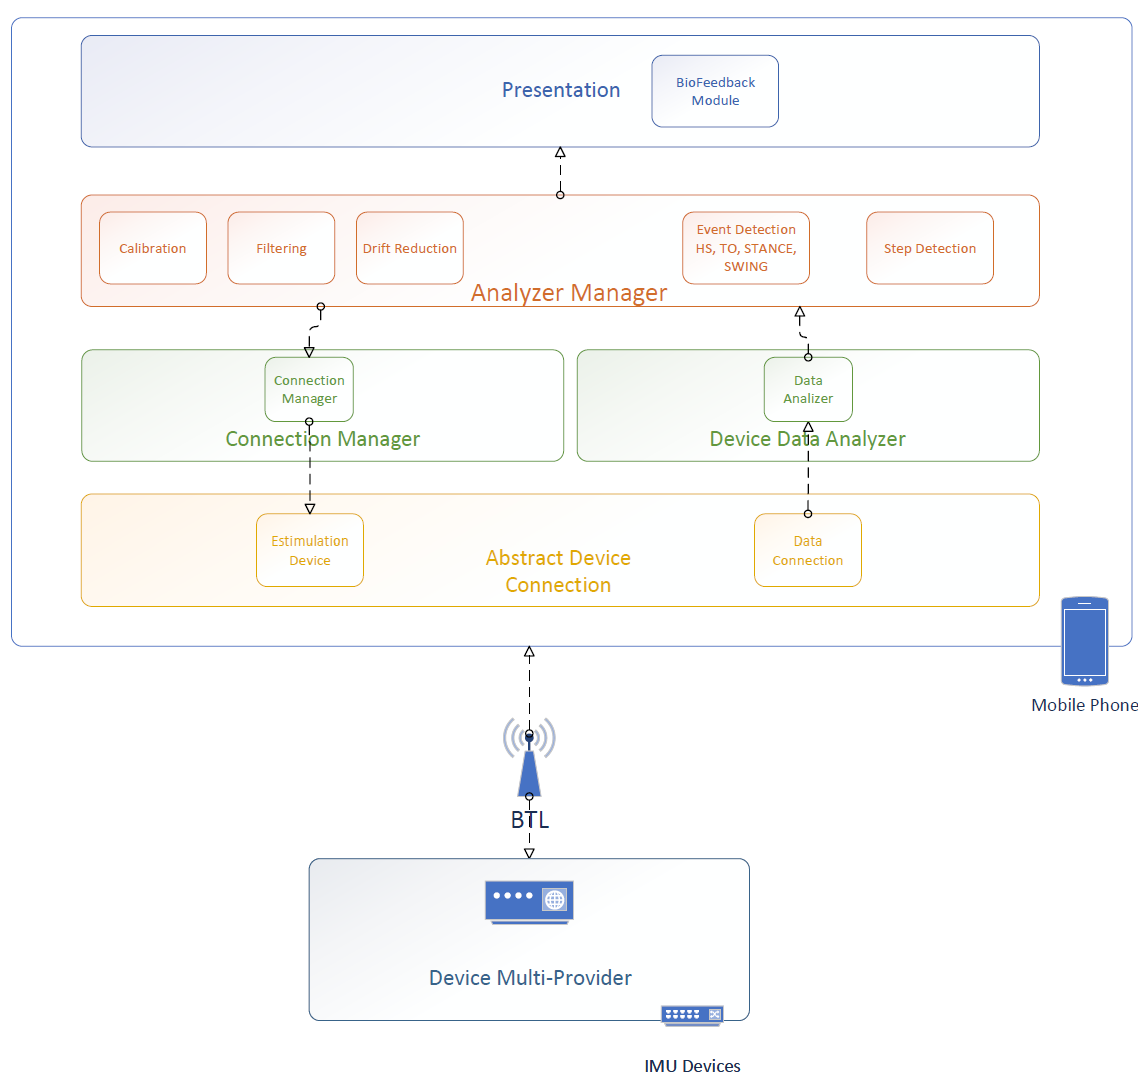
\includegraphics{TESIS/imagenes/img/Arquitectura2.png}}
\caption{Arquitectura del sistema PARKIBIP. Se compone de seis capas bien definidas desde el controlador del hardware hasta la capa de presentación. }
\label{FIG:Arquitectura2}
\end{figure}

En el diseño se pueden identificar seis capas específicas, con responsabilidades bien delineadas. Primero, y externo al Software de la aplicación Android, los dispositivos IMU con conectividad Bluetooth compuestos por los distintos sensores de movimiento. Asimismo, se identifican tres módulos de bajo nivel, vinculados a la conectividad y búsqueda, interacción con los distintos dispositivos y recuperación de datos de los sensores empleados (``Abstract Device Connection'', ``Connection manager'', ``Device Data Analizer''). Luego, se encuentra un módulo de procesamiento de la información recopilada, vinculado al análisis y aplicación de algoritmos matemáticos que identifican los parámetros espacio temporales (``Analizer Manager''). Finalmente, un módulo de presentación de resultados, compuesto por un controlador clínico capaz de tomar decisiones y estimular adecuadamente al usuario.

\section{Componentes de PARKIBIP}

El dispositivo seleccionado en \nameref{section:imu-selection}, MetaMotionR (MMR), es un dispositivo portátil que ofrece un monitoreo continuo y en tiempo real de los datos de los sensores ambientales y de movimiento. Dentro de las características principales del MMR se encuentran:
\begin{itemize}
    \item SDK (del inglés, Software Development Kit) en lenguaje JAVA, de código abierto para la adquisición de datos de sensores
    \item Batería recargable de Litio
    \item Bajo consumo de energía, el modo de suspensión admite hasta 6 meses de inactividad
    \item Tamaño diminuto, 27mm × 27mm x 4mm
    \item Ultraliviano: 5.6 gramos
    \item 8MB de memoria interna
    \item Protocolo de transferencia: Bluetooth Low Energy 
\end{itemize}

Los sensores incluidos en el IMU son un giroscopio, un acelerómetro y un magnetómetro (todos de tres ejes); así como un sensor de presión barométrica, un sensor de luz ambiental y un sensor de humedad.

% QUE 3. Aplicación: que hace?
Se implementó una aplicación móvil Android en el lenguaje JAVA que se interconecta a dos dispositivos IMU a través del protocolo estándar Bluetooth Low Energy. El sistema se encuentra diseñado con el propósito de efectuar las siguientes actividades:

\begin{enumerate}
    \item Escanear dispositivos IMU y enlazarlos a la aplicación móvil para ambos miembros inferiores
    \item Calibrar los sensores de los IMU
    \item Recuperar los datos acelerómetro, giroscopio y magnetómetro de los respectivos sensores
    \item Estimar orientación del dispositivo respecto a una posición inercial mediante un método eficiente del gradiente descendiente 
    \item Identificar fase de la marcha en tiempo real mediante algoritmos numéricos específicos
    \item Estimar parámetros espacio-temporales de la marcha bajo algoritmos numéricos particulares
    \item Estimular al usuario de acuerdo a protocolo clínico
\end{enumerate}

\section{Interoperabilidad con dispositivos IMU} \label{section:app-imu}

Para estudiar e implementar el modo de operación entre la aplicación Android y los sensores IMU, se optó, en una primera etapa, por desarrollar una prueba de concepto o \gls{PoC} (del inglés, Proof of Concept). Esta prueba de concepto, tenía principalmente los siguientes objetivos: 

\begin{itemize}
    \item Familiarizarse con el escaneo de dispositivos Bluetooth desde la plataforma Android.
    \item Comprender de qué forma se interactúa desde una aplicación Android con un dispositivo Bluetooth.
    \item Conocer y utilizar el SDK para interactuar con el dispositivo IMU (MMR).
    \item Realizar una conexión exitosa con el dispositivo.
    \item Generar comunicación bidireccional, accionando sobre el dispositivo MMR (e.g. encendiendo la luz led) y recuperando datos desde uno de los sensores (e.g. acelerómetro) del dispositivo.
    \item Empaquetar o fusionar los datos de acelerómetro, giroscopio y magnetómetro a una frecuencia determinada.
    \item Escalar el numero de dispositivos inerciales conectados y operando en simultaneo.
\end{itemize}

El sistema operativo Android incluye soporte para el stack de red Bluetooth, permitiendo que un dispositivo intercambie datos de forma inalámbrica con otros dispositivos dentro del alcance del mencionado protocolo. Se proporciona acceso a la funcionalidad Bluetooth a través de un framework que es parte del kit de Android, habilitando a las aplicaciones a conectarse de forma inalámbrica a otros dispositivos Bluetooth. Esto es, funciones inalámbricas de punto a punto y multipunto.

\noindent Para utilizar las funcionalidades de Bluetooth, se requiere solicitar autorización al usuario, para esto es necesario declarar los permisos pertinentes en el archivo de configuración de la aplicación, conocido como Manifiesto (en inglés, Manifest). 

Uno de los grandes beneficios contemplados en la evaluación del dispositivo seleccionado -MMR del proveedor \textit{MetaWear}-, es el SDK de código abierto para el \textit{MetaWear}. Un kit de desarrollo de software contiene archivos de cabecera, bibliotecas, muestras, documentación y herramientas que simplifican el desarrollo -en este caso la integración y la comunicación con el hardware inercial-, que de otra forma seria muy complejo de efectuar. En general, es provisto por el proveedor del hardware conforme a comunicarse con el sistema embebido en un lenguaje de bajo nivel. 

Por lo tanto, se desarrolló la integración con el hardware inercial, mediante la incorporación de la SDK de \textit{MetaWear} al proyecto Android, a través del gestor de dependencias remotas \gls{Gradle}. Luego, fue necesario configurar e inicializar adecuadamente el servicio \textit{BtleService}, con el fin de escanear y enlazar dispositivos existente dentro del rango Bluetooth -ver diseño en la Fig. \ref{fig:activity-scanning}-. Con los dispositivos enlazados correctamente, es factible comenzar a interactuar mediante diversas funciones de la interfaz. 

\begin{figure}[!h]
     \centering
     \begin{subfigure}[t]{0.4\textwidth}
         \centering         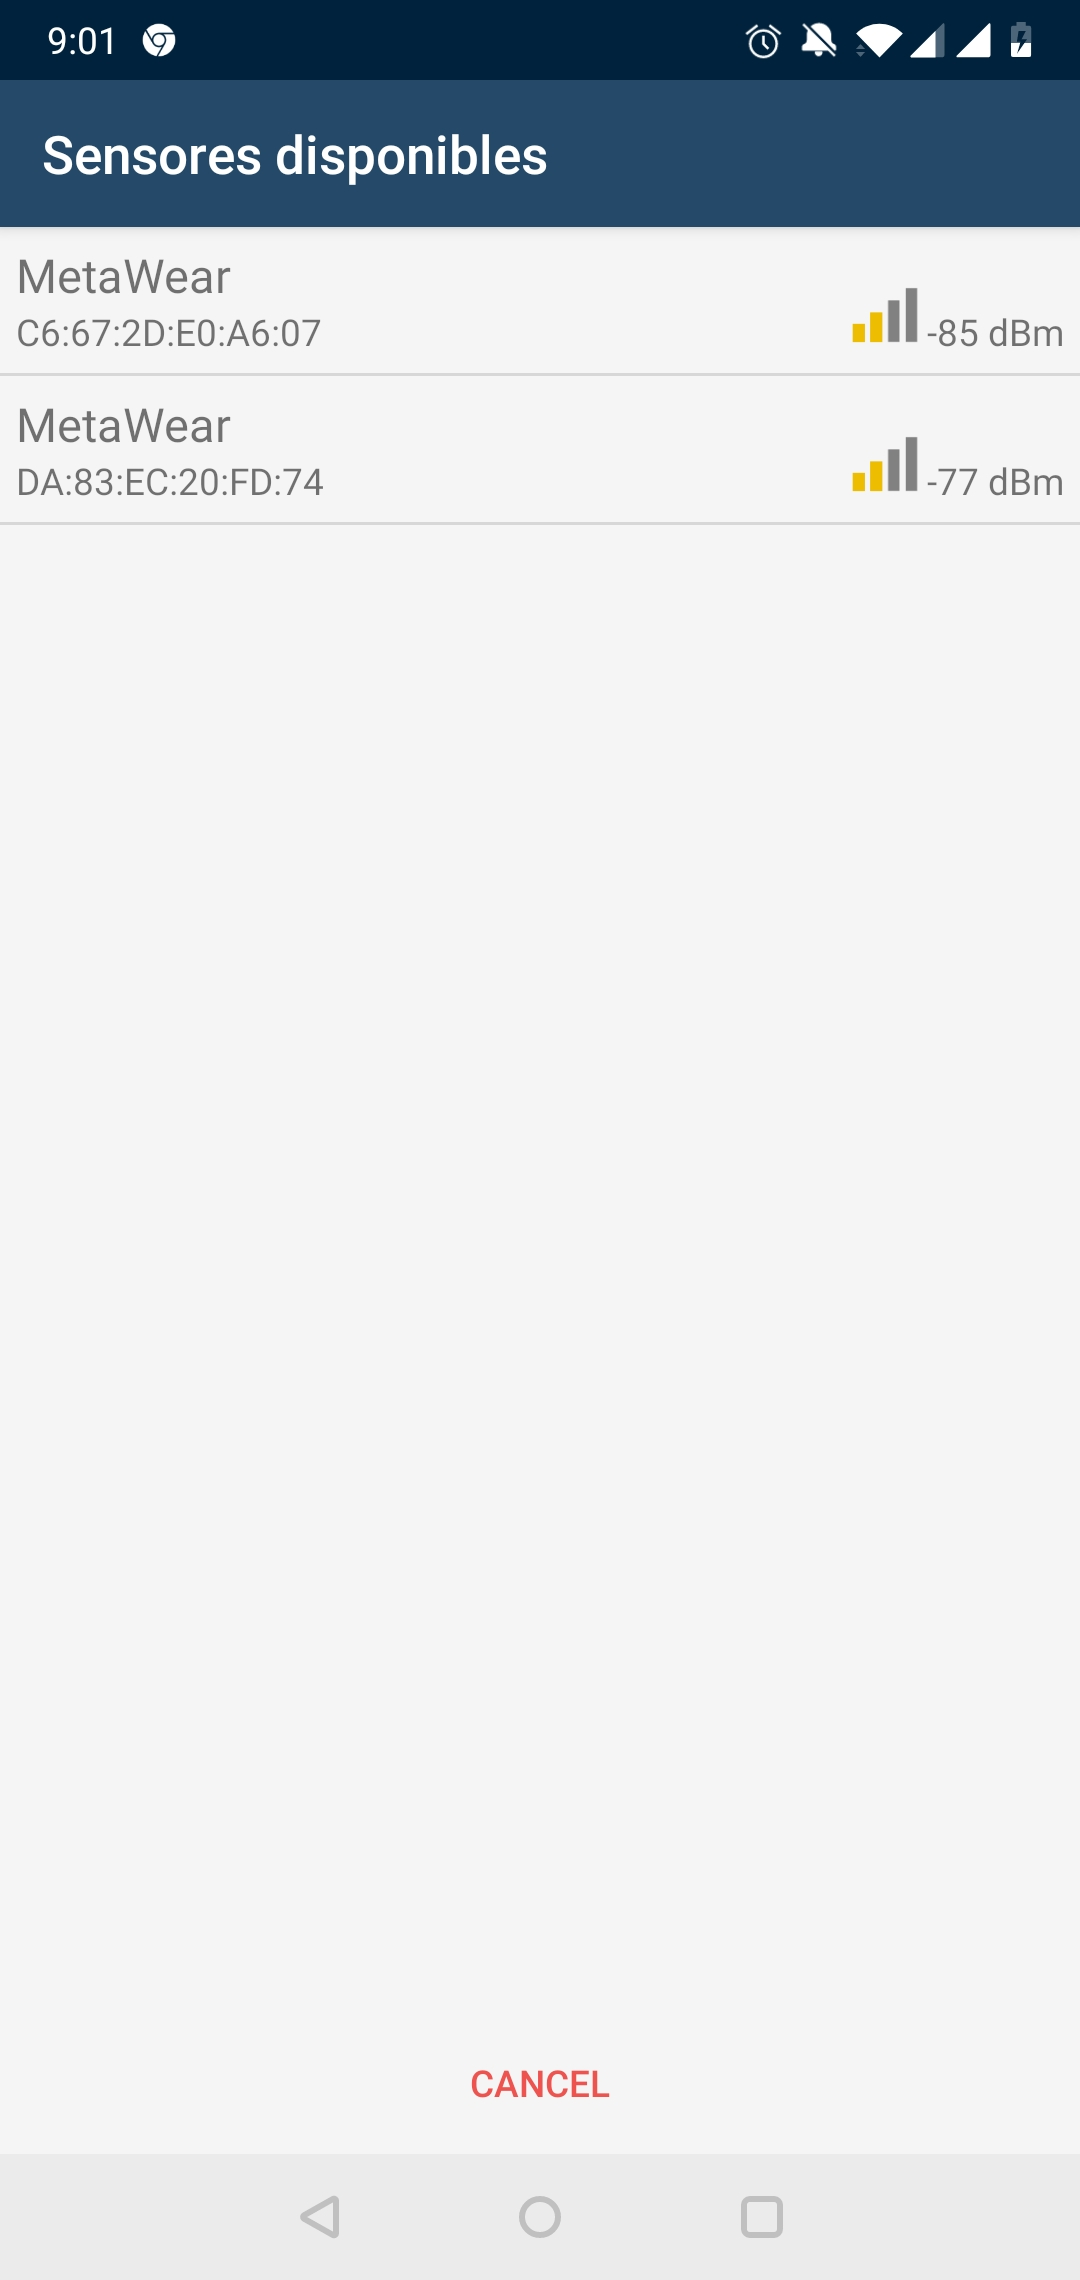
\includegraphics[height=8cm]{TESIS/imagenes/chap05/activity-searching-imus.JPG}
         \caption{Escaneo de dispositivos IMU. Previa activación del módulo bluetooth, expone un listado de IMU en la cercanía. Para cada uno muestra su dirección MAC, el tipo de IMU y la intensidad de la señal.}
     \end{subfigure}
     ~
     \begin{subfigure}[t]{0.4\textwidth}
         \centering
         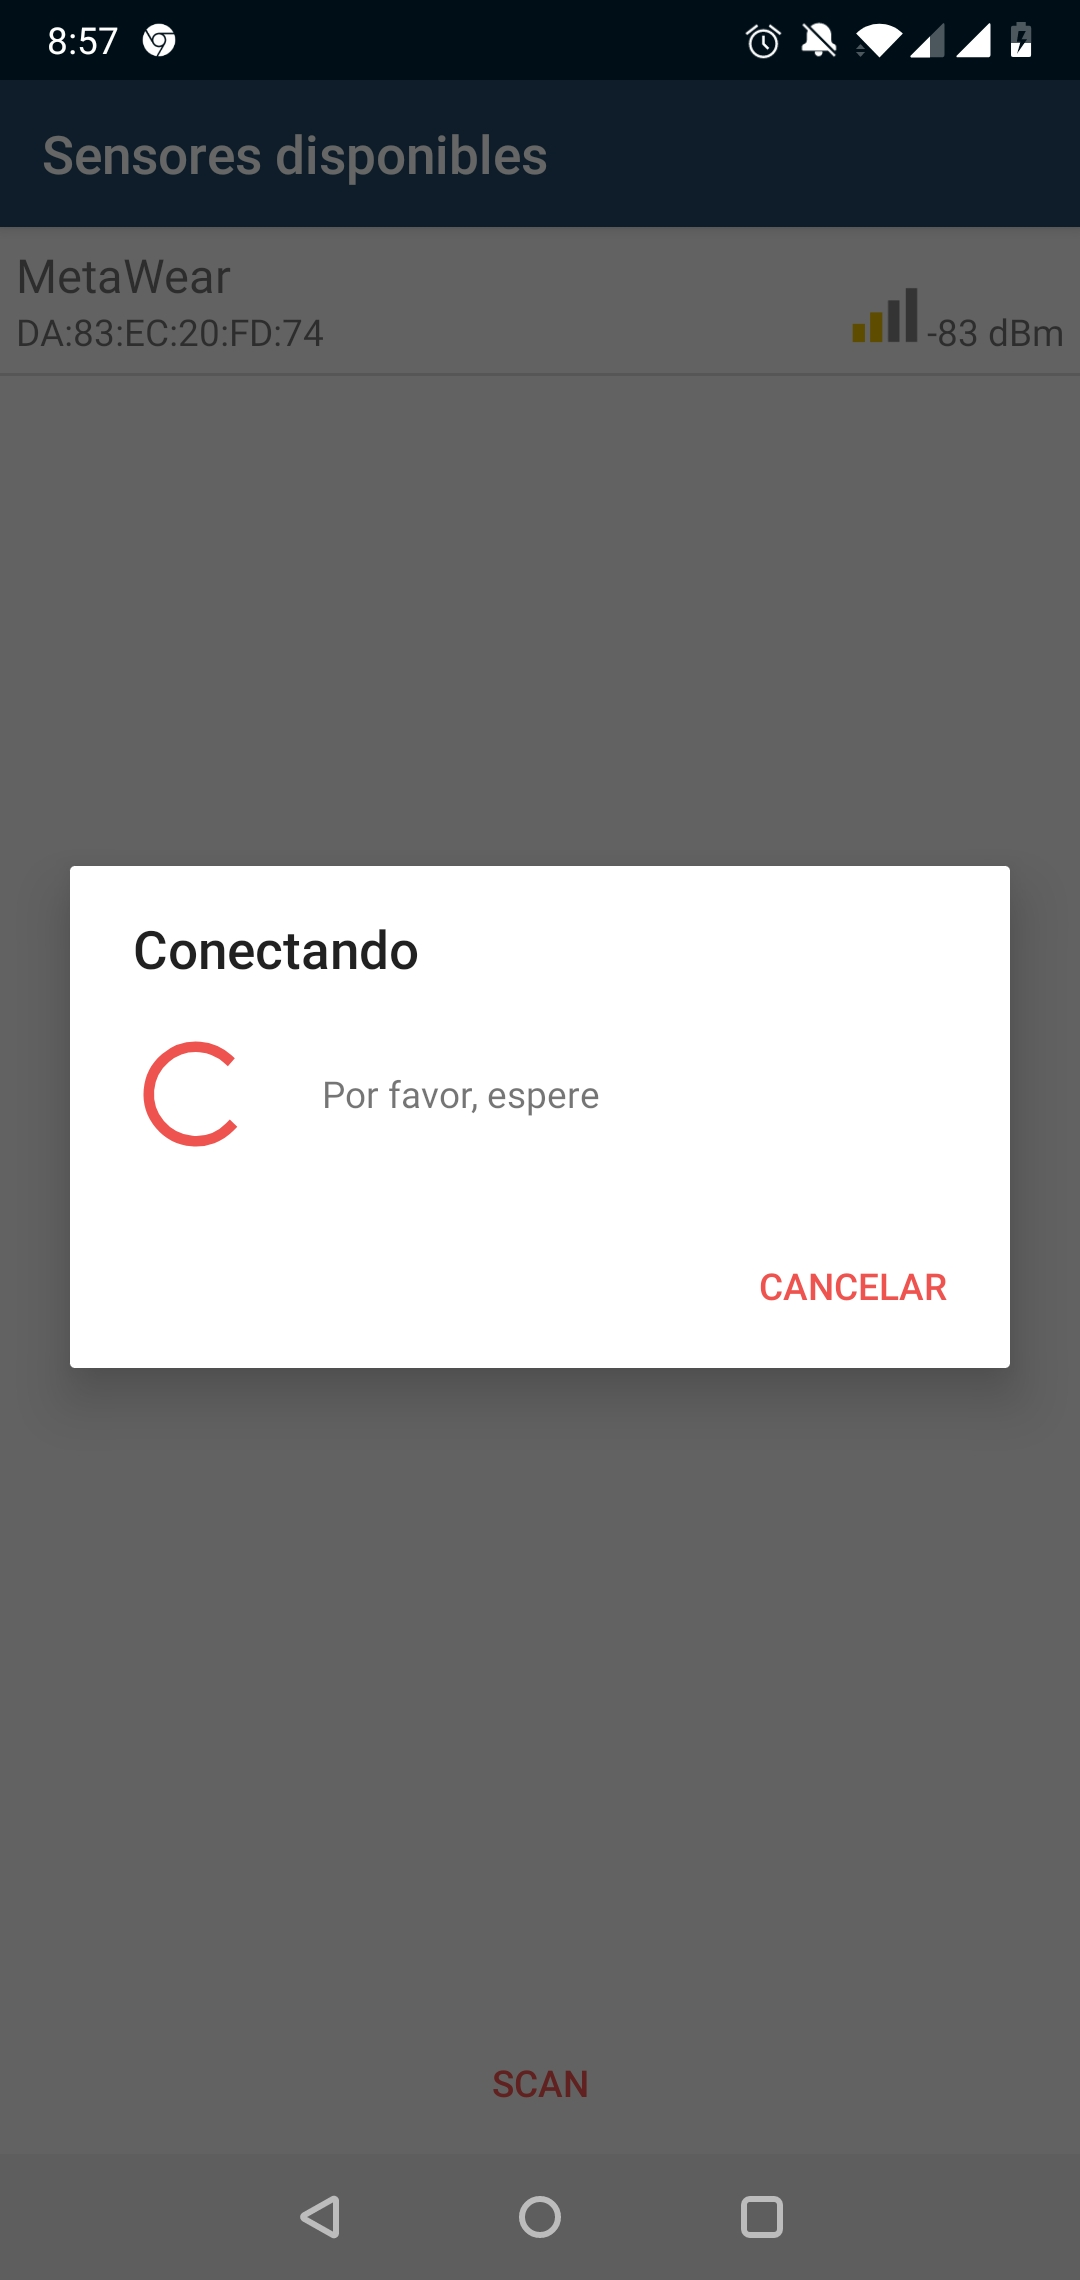
\includegraphics[height=8cm]{TESIS/imagenes/chap05/activity-connecting.JPG}
         \caption{Conexión en curso a un dispositivo IMU. Finalizada el proceso, el IMU es conectado exitosamente a PARKIBIP.}
     \end{subfigure}
     \caption{Proceso de escaneo previa a conexión de un IMU. Mediante el protocolo Bluetooth.}
     \label{fig:activity-scanning}
 \end{figure}

A continuación, se listan los módulos y algunas de las funciones principales que se emplearon en PARKIBIP:

\begin{enumerate}
    \item Bluetooth LE Connection: Gestión de la conexión entre aplicación Android y dispositivos IMU. 
    \begin{itemize}
        \item connectAsync: Establecimiento de conexión a un dispositivo.
        \item disconnectAsync: Remover la conexión a un dispositivo.
        \item UnexpectedDisconnect: Administración de eventos de desconexión inesperados.
        \item readDeviceInformationAsync: Obtener nivel de batería e información general del dispositivo.
        \item tearDown: Remueve los recursos asignados por el firmware del dispositivo.
    \end{itemize}
    \item \textit{DataProducer}: Componentes que recuperan datos, ya sean de sensores o de funciones del firmware.
    \begin{itemize}
        \item \textit{AsyncDataProducer}: Los productores de datos asincrónicos, cuando están activos, miden constantemente los datos en \gls{background} y los envían cuando hay nuevos datos disponibles.
        \item start: Inicia un productor de datos previamente configurado (e.g. sensor acelerómetro).
        \item stop: Remueve un productor de datos sin remover la conexión al hardware.
    \end{itemize}
    \item \textit{DataRoute}: Las rutas de datos proporcionan una forma simple y compacta para el acceso a las funciones avanzadas de \textit{MetaWear}, como el registro \textit{Log}, el procesamiento de datos y el manejo de eventos a bordo.
    \begin{itemize}
        \item addRouteAsync: creación de rutas de eventos, que definen cómo fluyen los datos desde un productor a diferentes puntos finales (a través de un \textit{RouteComponent}).
        \item Data: Los datos creados por los productores de datos están representados por la interfaz ``Datos'', que encapsula atributos de clave-valor, como la hora en que fueron creados los datos (timestamp) y el valor de la muestra de datos.
        \item stream: Permite el procesamiento del flujo de datos y como serán transformados los mismos. Establece un suscriptor al evento del productor de datos.
        \item log: Habilita a grabar datos en la memoria flash incorporada y recuperarlos en un momento posterior.
        \item state: Permite recuperar el vector de estados del dispositivo.
        \item buffer: Los almacenes son unidades que graban la entrada más reciente en su estado interno, y posteriormente permiten acceder mediante el método de estado (\textit{state}) perteneciente al módulo procesador de datos.
    \end{itemize}
    \item Function Module: Existen tantos módulos como sensores. Se listan funcionalidades genéricas a los módulos (Acelerómetro, giroscopio, magnetómetro, barómetro, luz ambiental, entre otros).
    \begin{itemize}
        \item start: Establece el uso de un módulo especifico.
        \item stop: Remueve el uso de un módulo especifico.
        \item configure: Configuraciones particulares a cada módulo.
        \item odr: Tasa de datos de salida.
        \item range: Rango de datos.
    \end{itemize}
\end{enumerate}

Es importante notar que, algunos de los nombres de los métodos disponibles finalizan con la palabra ``Async'', y significa que \underline{toda comunicación es asincrónica con el dispositivo}. Esto es un requisito a nivel del sistema operativo y es una característica esencial del sistema PARKIBIP, ya que el acceso a los datos del dispositivo no puede ser bloqueante. 

De esta manera, \underline{PARKIBIP es un sistema multihilo} (multithreading en inglés), teniendo la capacidad de ejecutar eficientemente múltiples hilos de ejecución y paralelizar diversas tareas en background, como por ejemplo los mensajes hacia o desde un dispositivo. Asimismo, esta tarea se complejiza aún mas, al escalar en número los dispositivos inerciales que puede gestionar el sistema. Entonces, se implementaron diversos hilos, para lograr:

\begin{itemize}
    \item Gestionar múltiples conexiones a dispositivos inerciales.
    \item Interactuar con los dispositivos mediante el envío y recepción de mensajes apropiados.
\end{itemize}

Se resalta la necesidad de diseñar e implementar diferentes estrategias para el control de concurrencia sobre recursos compartidos de los diversos Threads en simultanea ejecución.

\section{Administración de las conexiones}

Como se resaltó en la sección anterior \nameref{section:app-imu}, las conexiones entre la aplicación Android y un dispositivo Bluetooth se representan en una aplicación Android mediante la clase perteneciente al SDK de Android llamada \textit{BluetoothDevice}. Esta clase representa un dispositivo remoto conectado por Bluetooth, permitiendo a la aplicación comunicarse con el dispositivo, operar sobre él y requerirle datos como el nombre, dirección, clase, estado, batería, etc. 

Esta clase es realmente un fino \gls{wrapper} delgado para una dirección de hardware Bluetooth. Los objetos de esta clase son inmutables. Las operaciones en esta clase se realizan en la dirección de hardware Bluetooth remota, utilizando la clase \textit{BluetoothAdapter}. 

Para obtener un dispositivo Bluetooth, se utiliza la clase \textit{BluetoothAdapter}, con el método \textit{getRemoteDevice(String)}, la cual crea una instancia de \textit{BluetoothDevice} que representa un dispositivo de una dirección MAC conocida (que se puede obtener a través del descubrimiento de dispositivos también utilizando \textit{BluetoothAdapter}). Este descubrimiento se realiza en una pantalla dedicada dentro de la aplicación (en android representada con la clase \textit{Activity}), la cual llamamos \textit{ScannerActivity}. 

En la pantalla inicial de la aplicación, llamada \textit{MainActivity}, se le muestran al usuario botones para conectar cada uno de los dispositivos necesarios para el funcionamiento de PARKIBIP, uno para el pie izquierdo y otro para el pie derecho -ver Fig. \ref{fig:activity-conection-imu}-. 

\begin{figure}[!h]
     \centering
     \begin{subfigure}[t]{0.4\textwidth}
         \centering
         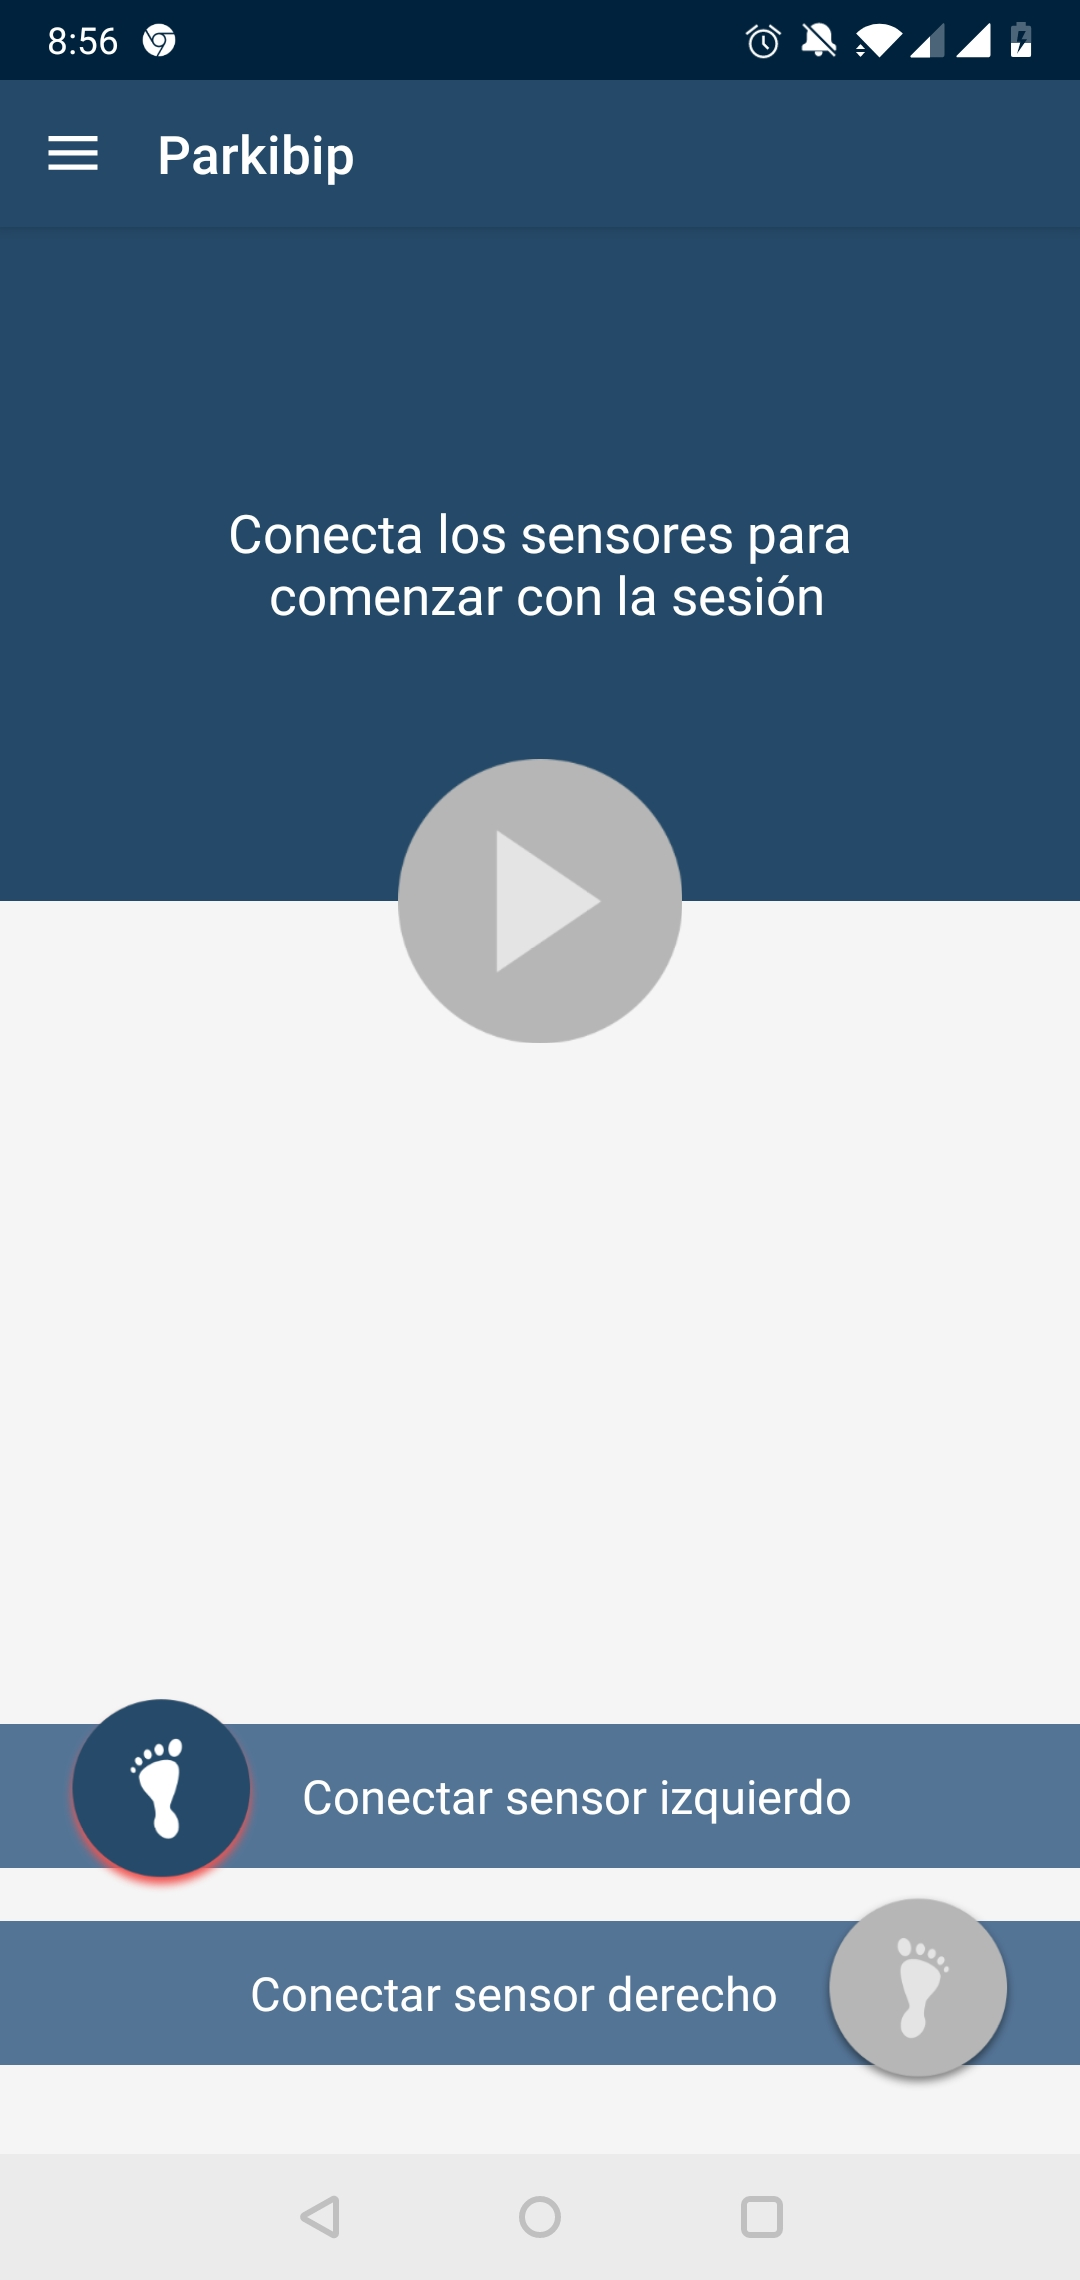
\includegraphics[height=8cm]{TESIS/imagenes/chap05/activity-selected-imu.JPG}
         \caption{Conexión exitosa del IMU asociado al pie izquierdo -botón coloreado de azul-. PARKIBIP identifica al Pie/IMU con un color en la aplicación, en la imagen rojo. Es el mismo color que comienza a parpadear en el IMU mediante su luz LED.}
     \end{subfigure}
     ~
     \begin{subfigure}[t]{0.4\textwidth}
         \centering
         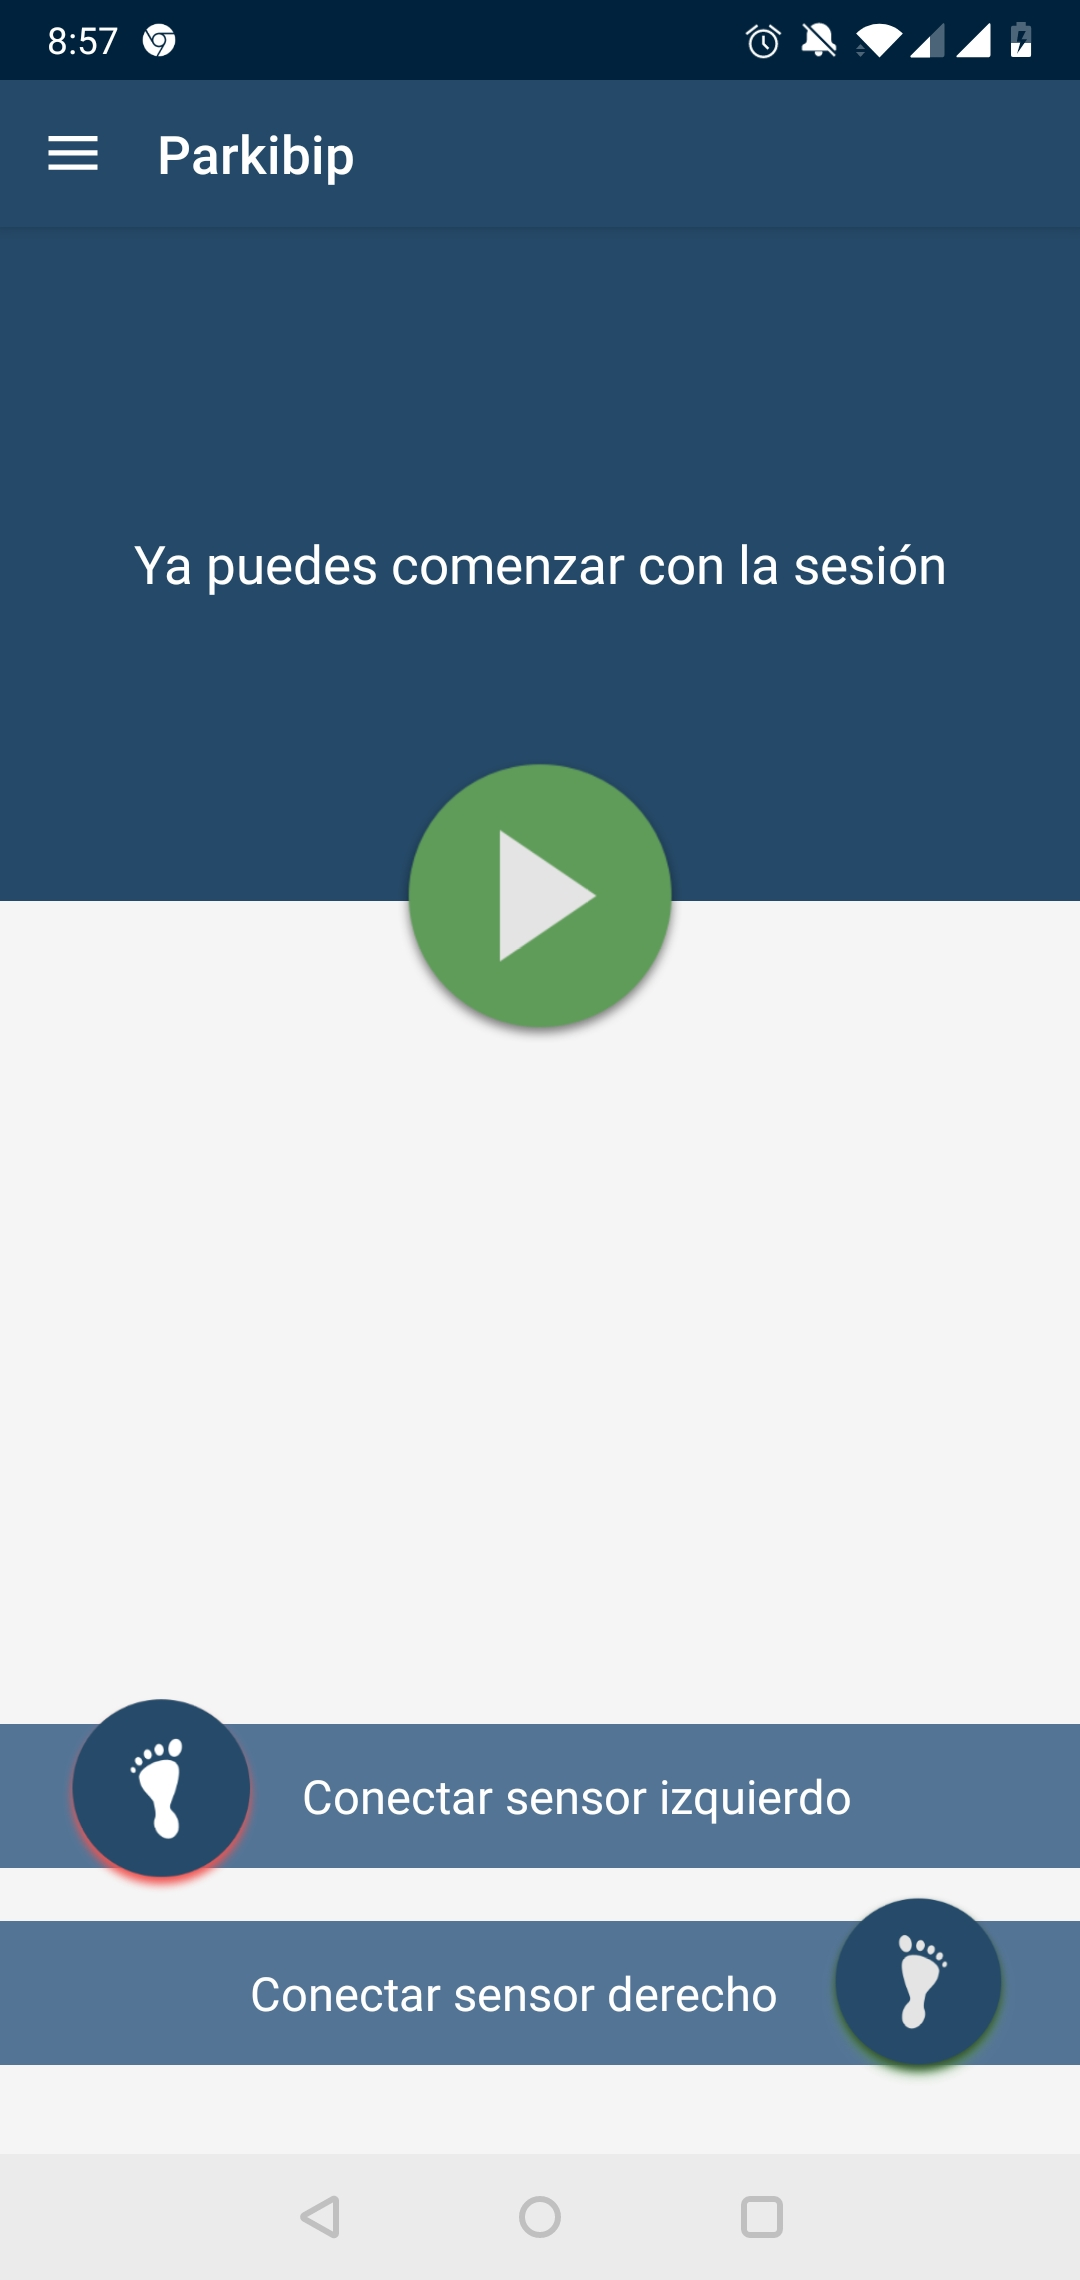
\includegraphics[height=8cm]{TESIS/imagenes/chap05/activity-ready-for-use.JPG}
         \caption{Conexiones a los IMU exitosa. Ambos botones se encuentra en azul, las luces LED del IMU sincronizadas a los colores de los contornos de los botones, y el botón central es puesto en verde. PARKIBIP se encuentra listo para comenzar una sesión de rehabilitación.}
     \end{subfigure}
     \caption{Conexiones a los dispositivos IMU mediante el protocolo Bluetooth.}
     \label{fig:activity-conection-imu}
 \end{figure}

Al seleccionar uno de estos botones se le muestra al usuario la pantalla de escaneo y selección de dispositivos IMU. Es importante destacar que el descubrimiento de dispositivos Bluetooth lo realizamos en esta pantalla filtrando la clase específica de dispositivos que requiere Parkibip, para que solo se listen dispositivos Bluetooth del tipo IMU y no algún otro dispositivo que pueda estar cerca del Smartphone. Una vez que la conexión se establece, la pantalla principal muestra un indicador de que el sensor para ese pie se encuentra conectado. Este indicador tiene un color específico que también se muestra a través de una luz Led en el sensor MMR (color rojo para el pie izquierdo y color verde para el pie derecho) que permite identificar qué sensor se debe colocar en cada pie. 

En el listado de cada uno de los dispositivos se muestra información pertinente sobre los dispositivos encontrados, como lo es su dirección MAC, el tipo de dispositivo, la intensidad de la señal (importante para el buen funcionamiento de la aplicación), entre otras cosas. 

Cuando el usuario selecciona un dispositivo, se realiza la conexión con el dispositivo y se obtiene una instancia de la clase \textit{BluetoothDevice} que utilizaremos para obtener los datos del dispositivo mientras el usuario realice la actividad. Resulta importante entonces proveer un mecanismo para administrar estas conexiones, mantener las instancias, identificarlas, liberarlas cuando sea necesario y que se realice su re-conexión en caso de que sea interrumpida. Con todos estos objetivos diseñamos el sistema como se muestra en la figura Fig. \ref{FIG:connections-management} 

\begin{figure}[H]
    \hspace*{-3.5cm}%
    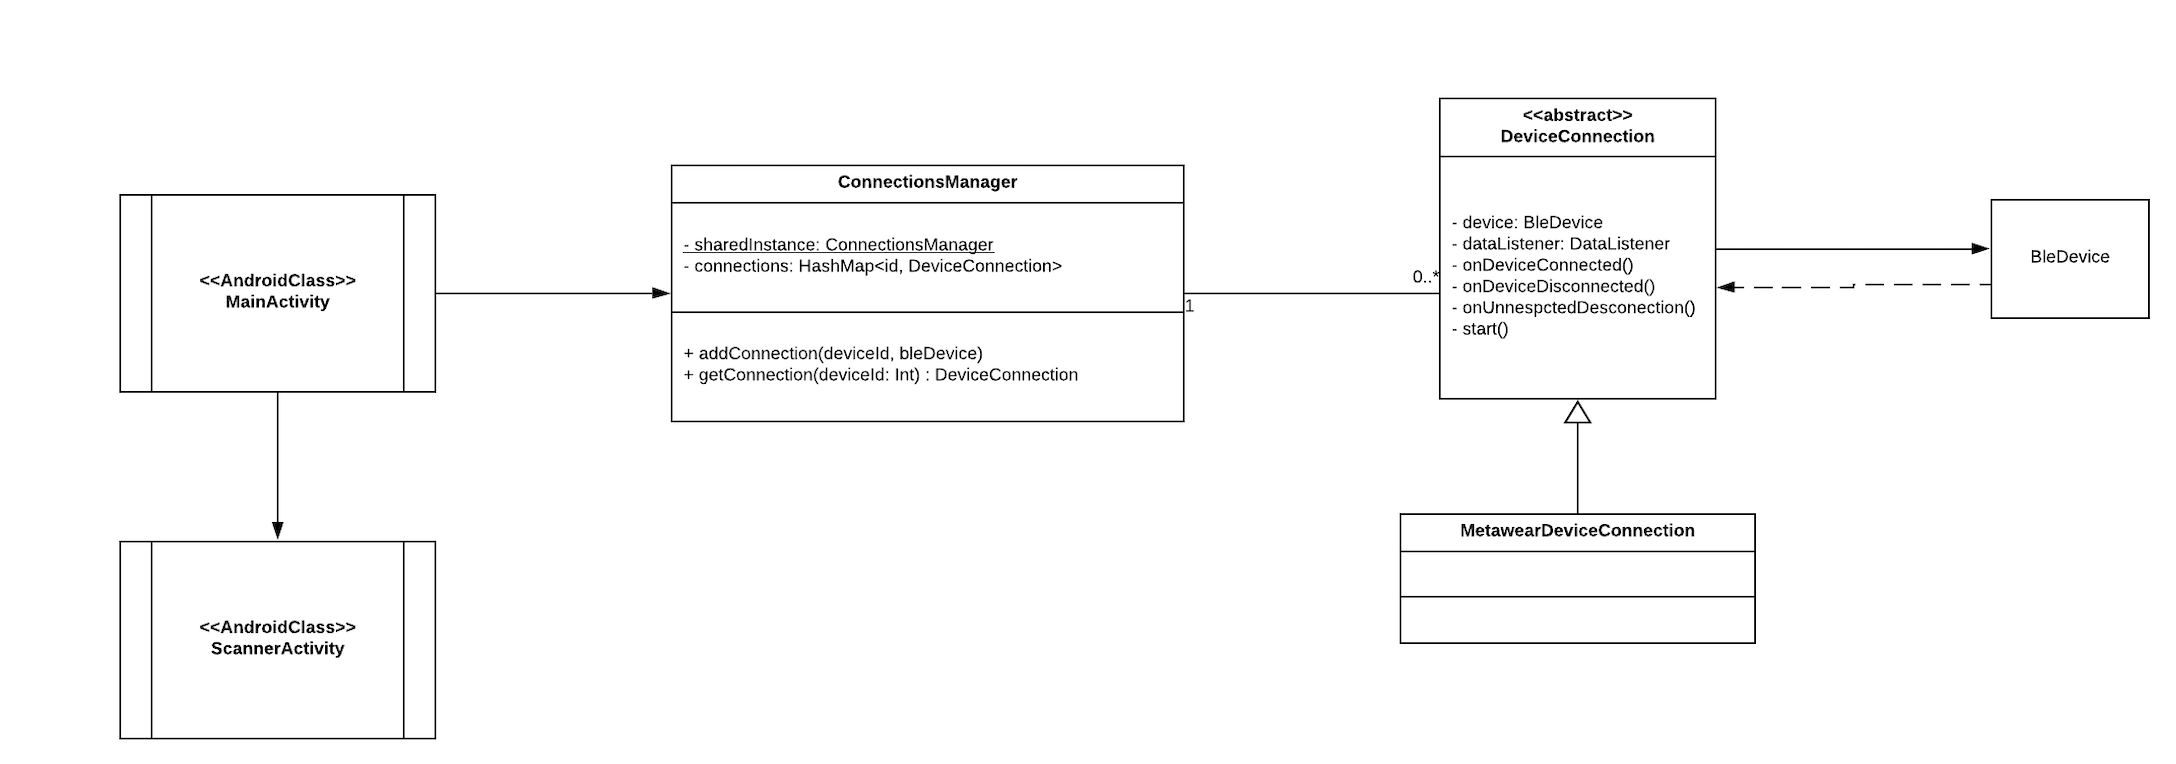
\includegraphics[clip,width=1.4 \columnwidth]{TESIS/imagenes/chap05/connections-management-design.png}
    \caption{Diagrama de clases del módulo de la aplicación Android donde se administran las conexiones Bluetooth con los dispositivos IMU}
    \label{FIG:connections-management}
\end{figure}

A continuación se describen las principales características del diseño, la interacción entre las clases y sus roles: 

\begin{itemize}
    \item La pantalla principal representada con la clase \textit{MainActivity} es encargada de crear y mostrar la pantalla de escaneo y selección de dispositivos (\textit{ScannerActivity}).
    \item En la pantalla \textit{ScannerActivity} el usuario selecciona el dispositivo y se crea la instancia de \textit{BluetoothDevice}.
    \item La pantalla \textit{MainActivity} recibe la instancia de \textit{BluetoothDevice} y se la provee a \textit{ConnectionsManager}. 
    \item \textit{ConnectionsManager} es un \textit{Singleton} con la única responsabilidad de administrar las conexiones existentes, guardadas en un Diccionario Clave-Valor (utilizando como clave un identificador de tipo \textit{String}).
    \item Cada conexión es mantenida por una instancia de la clase \textit{DeviceConnection}, una clase abstracta que representa el concepto de conexión con un dispositivo IMU. Estos objetos tienen la capacidad de mantener la conexión activa, solicitarle los datos al sensor, terminar el flujo, reconectarlo en caso de que la conexión sea interrumpida, entre otras cosas. 
    \item Para el dispositivo MetaMotionR se implementó una clase concreta de \textit{DeviceConnection} llamada \textit{MetaWearDeviceConnection}. La misma tiene una implementación concreta con las particularidades requeridas para comunicarse con este tipo de dispositivos, utilizando el SDK de MetaWear mencionado anteriormente.
\end{itemize}

El diagrama de comunicación de la Fig. \ref{FIG:addconnection-comm-diagram} detalla las distintas interacciones para el caso de uso ``Establecer conexión con dispositivo IMU''. 

\newpage

\begin{figure}[H]
    \hspace*{-3.0cm}%
    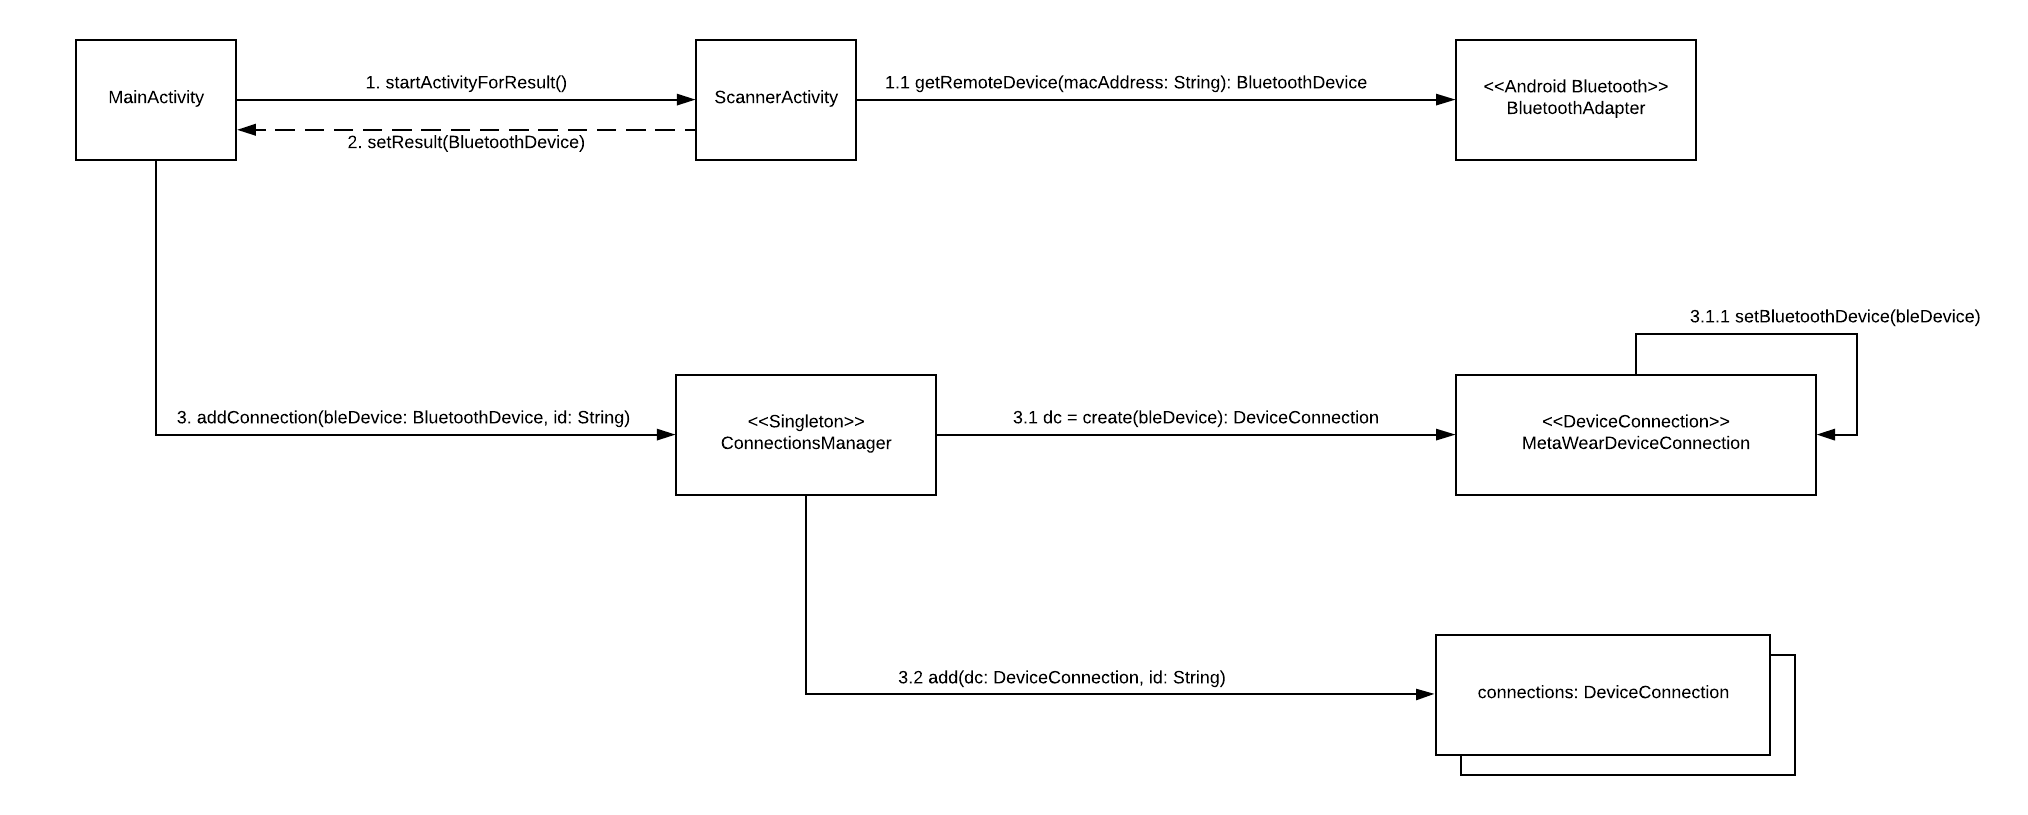
\includegraphics[clip,width=1.4 \columnwidth]{TESIS/imagenes/chap05/CreateConnection-CommDiagram.png}
    \caption{Diagrama de comunicación para el caso de uso ``Establecer conexión con dispositivo IMU''}
    \label{FIG:addconnection-comm-diagram}
\end{figure}

Este diseño nos provee de varias ventajas, a continuación nombramos algunas de éstas:

\begin{itemize}
    \item Las responsabilidades de cada clase están claras.
    \item Cada clase tiene una única responsabilidad.
    \item Agregar un nuevo tipo de dispositvo IMU -ya sea de otro proveedor de hardware, así como otro modelo de MbienLab- implicaría simplemente implementar una nueva clase concreta de la clase abstracta \textit{DeviceConnection}, lo que hace que el sistema sea escalable.
    \item Si en un futuro se quisiera utilizar más de dos dispositivos, este diseño funciona sin grandes cambios, ya que el manejador de conexiones \textit{ConnectionManager} puede mantener tantas conexiones como sea necesario 
    \item Este diseño soporta mantener conexiones con distintos tipos de dispositivos o de diferentes marcas de forma simultánea.
\end{itemize}
\newpage

% Como 1.Presentar Algoritmo de Fusión de datos
\section{Algoritmo de empaquetado de datos PARKIBIP}

Ya mencionado, la recopilación de datos de múltiples sensores de un dispositivo inercial, se realiza en diversos hilos de ejecución. Además, cada sensor opera con tasas de frecuencias eventualmente distintas -Hz-. Es fundamental combinar los datos recibidos -en hilos y frecuencias distintas- de manera adecuada, tal que los datos se mantengan consistentes.

Por lo tanto, se implementó un algoritmo de empaquetado de datos, con el objetivo de combinar valores de los sensores acelerómetro, giroscopio y magnetómetro en un único mensaje en cada instante de tiempo. Al fusionar varias fuentes de datos, es una restricción muestrear a la misma frecuencia, o al menos, múltiplos enteros de la frecuencia más rápida. 

El algoritmo desarrollado opera de la siguiente manera:
\begin{enumerate}
    \item Siempre se propagan los mensajes fusionados según la frecuencia mas alta
    \item El muestreo de fuentes de datos en las frecuencias más bajas repetirá el último valor recibido
    \item Se emplean dos colas de almacenamiento de mensajes, en modalidad de buffer FIFO (del inglés first-in, first-out), para las fuentes de datos cuyas frecuencias son mas bajas
\end{enumerate}

A continuación, se presenta el diagrama dado por la figura Fig. \ref{FIG: sensor-fuser}, el cual ejemplifica el procedimiento del fusión de datos.

\begin{figure}[H]
    \centering
    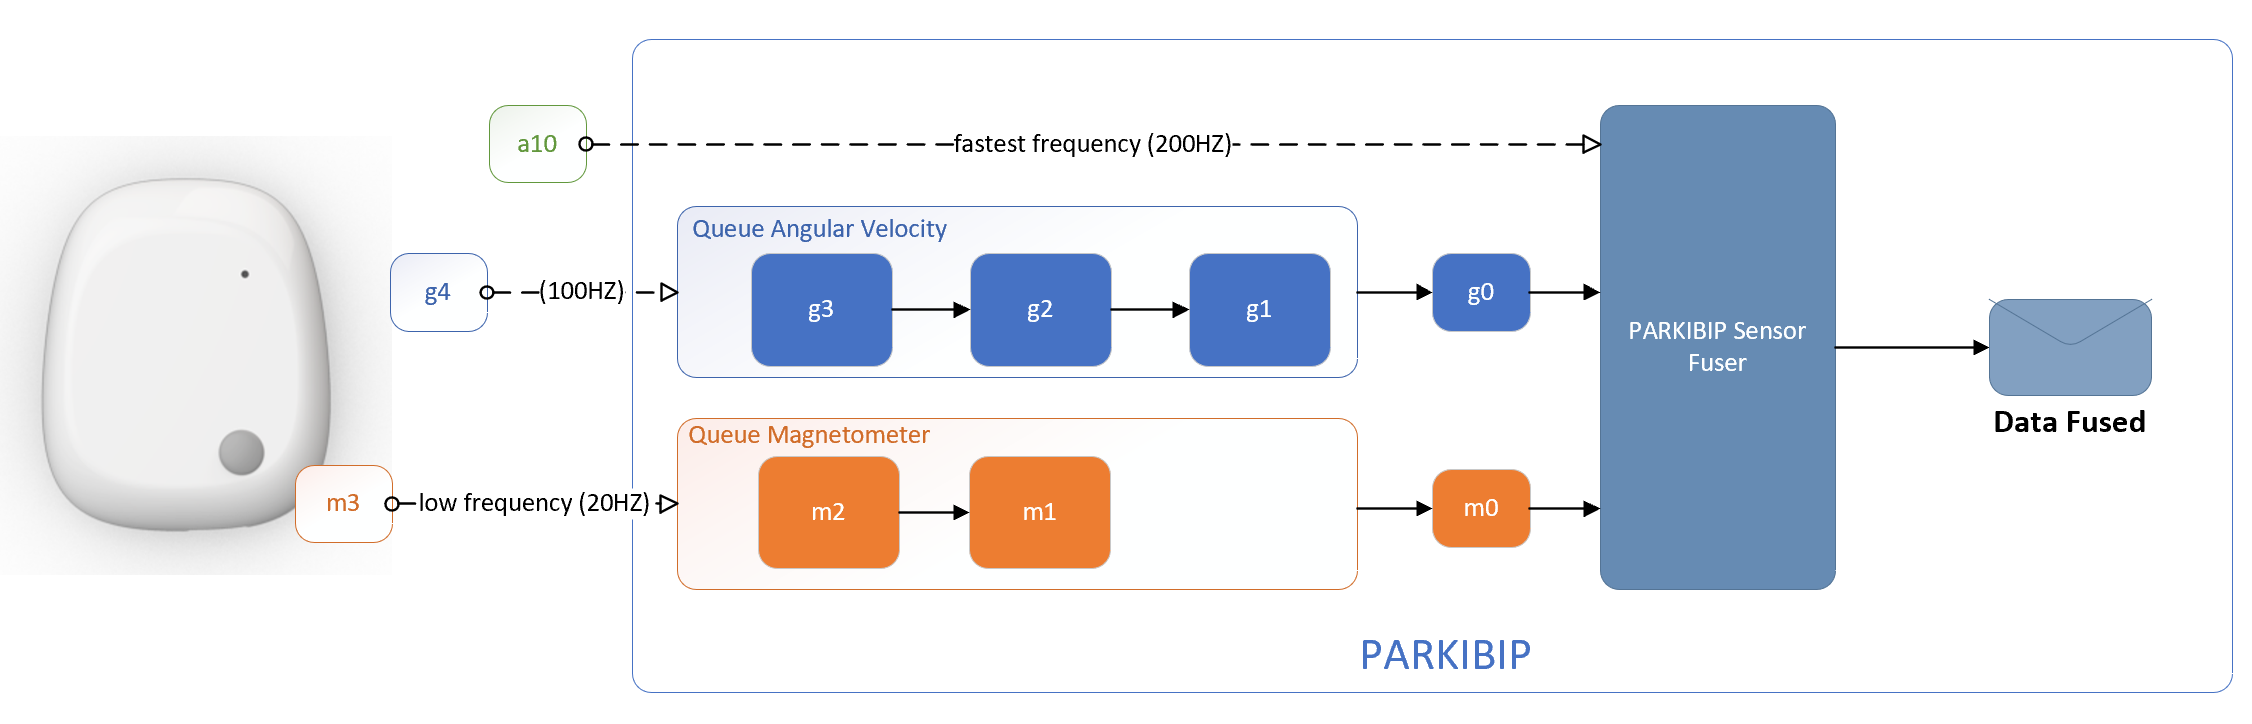
\includegraphics[clip,width=1.1 \columnwidth]{TESIS/imagenes/chap05/sensor-fuser.PNG}
    \caption{Algoritmo de empaquetado de datos PARKIBIP. Presenta un caso de uso de recopilación de datos de los sensores acelerómetro, giroscopio y magnetómetro en las frecuencias correspondientes 200HZ, 100HZ, 20HZ.}
    \label{FIG: sensor-fuser}
\end{figure}

% Como 2.0. API de Algoritmos (Quaternions, matrices, etc)
\section{Módulo de algoritmos numéricos y modelos de representación}\label{API-algoritmos} 

%Si o si hablar de cuaterion y propiedades, orientacion hace referencia
Puesto que PARKIBIP es un sistema físico-matemático complejo, el cual integra múltiples métodos numéricos y estadísticos; se optó por desarrollar un módulo destinado a la provisión de funciones independientes que aborden los problemas frecuentes. Este módulo, denominado ``API Algorithm'', tiene la responsabilidad de encapsular funciones reutilizables y particulares a la solución, para que luego sean accesibles desde cualquier método que las requiera.

En primer lugar, se introducen los principales modelos de representación que fueron empleados y gestionados dentro de la Interfaz de Programación de Aplicaciones (\gls{API}, Application Programming Interface) de algoritmos.
\noindent Conforme a representar la orientación del dispositivo en tiempo real, es necesario comprender los conceptos ángulos de euler (del inglés, Euler angles) y cuaternión (del inglés, Quaternion). Ambos modelos proporcionan una forma de representar la orientación de un cuerpo tridimensional mediante una combinación de tres rotaciones sobre diferentes ejes. Para el caso de los ángulos de euler, la secuencia de rotaciones utilizadas para representar una orientación dada es (i) yaw -rotación sobre el eje z un ángulo $\psi$-, (ii) pitch -rotación alrededor del eje Y un ángulo $\theta$-, (iii) roll -rotación alrededor del eje X un ángulo $\phi$-. Por otro lado, un quaternion es un vector de cuatro componentes, un elemento real y tres elementos complejos. Por ejemplo, $q^b_i = (a,bi,cj,dk)$  definido como el vector unitario que codifica la rotación desde el marco inercial hacia el marco del sensor. Luego, ambas representaciones pueden ser utilizadas para construir una matriz de rotación $R_{3X3}$ para realizar la rotación en una sola operación de multiplicación de matrices.

En vista de los modelos de representación introducidos y las necesidades operatorias del sistema, se implementaron las funciones necesarias para manipular y operar con éstos modelos de representación. En seguida, se listan algunas funciones desarrolladas en la API de algoritmos:

\begin{enumerate}
    \item Medición
    \begin{itemize}
        \item adjustMeasurementUnities(MeasurementModel measurementModel): Estandariza las unidades de las mediciones hacia los sistemas internacionales de unidades $m/s^2$ para aceleraciones y radianes para el caso de velocidades angulares.
        \item buildMeasurementWithData(Data data): Convierte una instancia genérica de la clase Data retornada por el IMU a su correspondiente modelo en PARKIBIP (MeasurementModel).
        \item buildMeasurement(Acceleration acceleration, AngularVelocity angularVelocity, MagneticField magneticField, Calendar timestamp): Crea una instancia lógica de MeasurementModel con el timestamp adecuado, a partir de los vectores tridimensionales acelerómetro, giroscopio y magnetómetro.
    \end{itemize}
    \item Filtro de Orientación
    \begin{itemize}
        \item updateOrientation(MeasurementModel measure, boolean hasMg): Función responsable de ejecutar el filtro de orientación implementado y retornar el nuevo quaternion. El parámetro \textit{hasMg}, indica la existencia de una observación del tipo magnetómetro.
    \end{itemize}
\item Aceleración  
\begin{itemize}
    \item romoveGravityForces: Método responsable de la extracción de la aceleración instantánea física del sensor.
    \item getUserAcceleration(MeasurementModel measure): Función encargada de obtener la aceleración del usuario en el marco inercial, resultado de la transformación de marcos y remoción de fuerzas gravitatorias.
    \item linearAccelerationMethod(MeasurementModel measure): Algoritmo responsable de computar la aceleración lineal instantánea del sensor.
\end{itemize}
\item Giroscopio
\begin{itemize}
     \item deg2rad(float degrees): Convierte el valor de grados a radianes para los datos del giroscopio.
    \item rad2Deg(float radians): Convierte el valor de radianes a grados para los datos del giroscopio.
\end{itemize}
\item Orientación
\begin{itemize}
    \item quaternProd(QuaternionModel q1, QuaternionModel q2): Función responsable de calcular el producto de dos cuaterniones.
    \item vectorFromRotationMatrix(RotationMatrix r, MeasurementModel measure): Dada una medición en el marco del sensor, aplica la Rotación por parámetro, para trasladar el vector a un marco de referencia inercial.
    \item vectorFromQuaternionProd(QuaternionModel q, MeasurementModel measure): Dada una medición en el marco del sensor, aplica la rotación dada por la orientacion en formato quaternion, para trasladar el vector a un marco de referencia inercial.
    \item convertToRotationMatrix(QuaternionModel q): Convierte un quaternion a su correspondiente matriz de rotación.
    \item convertToEulerAngles(QuaternionModel q): Convierte un quaternion a sus correspondientes ángulos de euler.
    \item getQuaternion(): Retorna el ultimo quaternion calculado por el filtro de orientación.
    \item dcm2q(double[][] rot): Convierte una matriz de cosenos de dirección al respectivo quaternion.
    \item rt2b(RealVector attitudeVector): Calcula y retorna la matriz de rotación desde un marco inercial al marco del sensor, a partir de los ángulos de euler.
\end{itemize}
\item Calibración
\begin{itemize}
  \item calibrateQuaternion(MeasurementModel measurementModel): Método iterativo responsable de calibrar adecuadamente la orientacion inicial del dispositivo IMU.
    \item stopCalibrateQuaternion(): Interrumpe un proceso de calibración retornando el ultimo quaternion computado.
    \item hasToStopCalibrate():  Chequea si es necesario interrumpir un procedimiento de calibración de orientación previamente iniciado. En caso de requerirse, retorna verdadero.
    \item hasToCalibrate(): Chequea si es necesario efectuar una calibración de orientación. En caso de requerirse, retorna verdadero.
\end{itemize}
\item Timestamp
\begin{itemize}
  \item getDiffSeconds(Calendar timestampOld, Calendar timestampNew): Obtiene la diferencia entre dos marcas de tiempos del tipo Calendar. 
\end{itemize}
\end{enumerate}

%TODO: agregar referencia a Apache 
Finalmente, para llevar adelante las distintas representaciones de matrices y vectores, asi como el algebra subyacente, se incluyó la librería de la compañía Apache, referida como ``Apache Commons Math'' \cite{apacheCommons}. La misma proporciona diversas funciones ligeras en el lenguaje de programación JAVA, representaciones numéricas escalables (e.g. naturales, reales, precisión simple y doble); por ende, facilita su utilización y reutilización independientemente de la complejidad requerida. 

En este sentido, es importante notar la complejidad de PARKIBIP relativa a la precisión numérica requerida, es decir, operaciones matriciales complejas y con valores numéricos que descienden aproximadamente a $10^{-22}$.

% Como 2.1.Marcos de referencia 
\section{Sistemas de coordenadas de referencias } \label{section:coordenadas}

Para lograr analizar la marcha de personas, así como también comprender el significado de las mediciones, es necesario identificar los sistemas de coordenadas que intervienen en el proceso.

%Sistema de coordendas
Puesto que los dispositivos inerciales IMU son colocados en los tobillos de los sujetos, existen tres sistemas de coordenadas: el marco de referencia Pie -que describe la rotación del pie-, el marco Sensor -que describe el movimiento del dispositivo inercial- y el marco fijo Inercial o Terrestre -ver figura Fig. \ref{fig:sensor-frame}-. Dado que el IMU se encuentra fijado al pie del sujeto mediante bandas elásticas de velcro, se asume que el dispositivo no se desliza ni se mueve durante la marcha. Por lo tanto, se considera que el sistema de coordenadas del pie es igual al sistema de coordenadas del Sensor.

%Procedimiento rotación y acele remover gravedad
El procedimiento consiste en recopilar las observaciones recibidas desde los distintos sensores, estimar la orientación de cada dispositivo en tiempo real; y luego transferir -mediante cuaterniones o rotaciones- el marco del sensor al marco inercial de la Tierra. Como consecuencia, es posible operar y realizar un análisis de la marcha desde un marco de referencia fijo, estandarizado y conocido.

\newpage

\begin{figure}[H]
\centering
\begin{subfigure}[b]{0.5\textwidth}
  \centering
  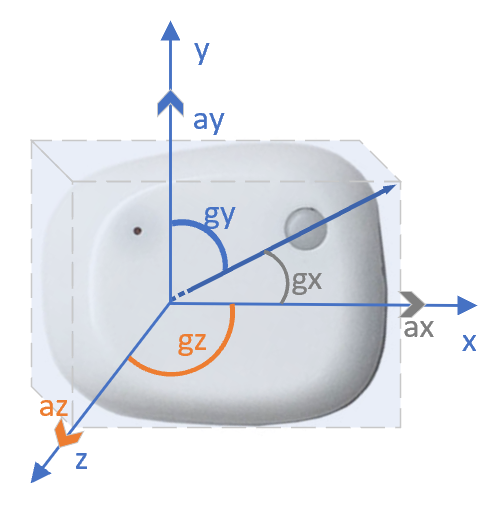
\includegraphics[width=\textwidth]{TESIS/imagenes/chap05/sensor-frame.PNG}
  \caption{Marco del Sensor IMU (S) de los ejes del acelerómetro y giroscopio, según especificación.}
  \label{fig:sfig1}
\end{subfigure}%
\begin{subfigure}[b]{0.5\textwidth}
  \centering
  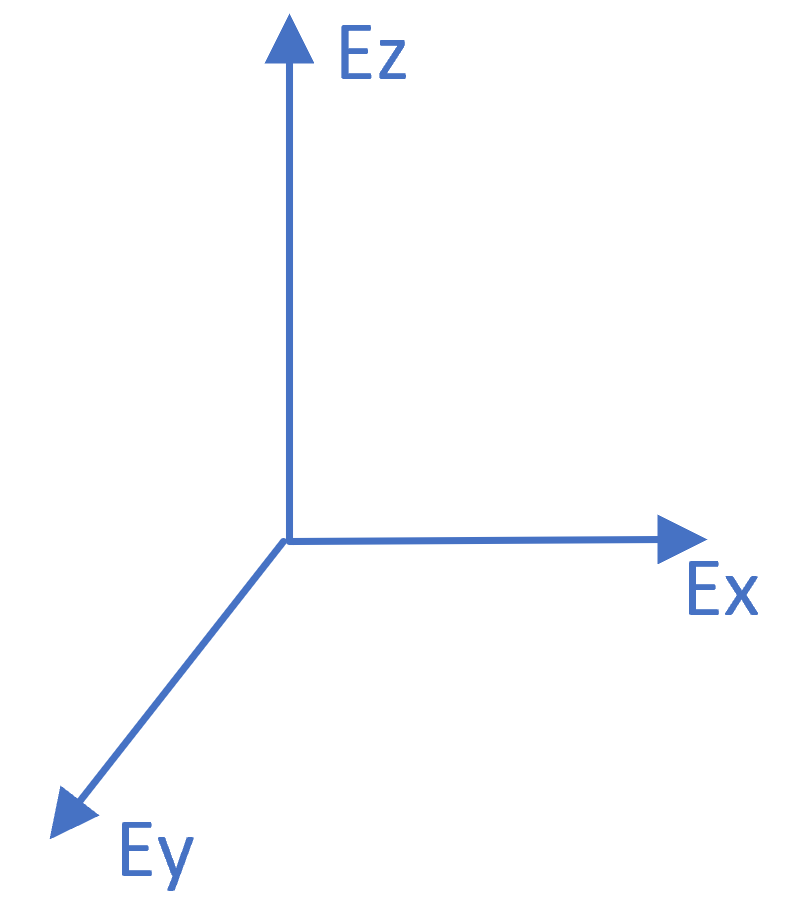
\includegraphics[width=\textwidth]{TESIS/imagenes/chap05/frame-earth.PNG}
  \caption{ Marco inercial Tierra (E). }
  \label{fig:sfig2}
\end{subfigure}
\begin{subfigure}[b]{0.5\textwidth}
  \centering
  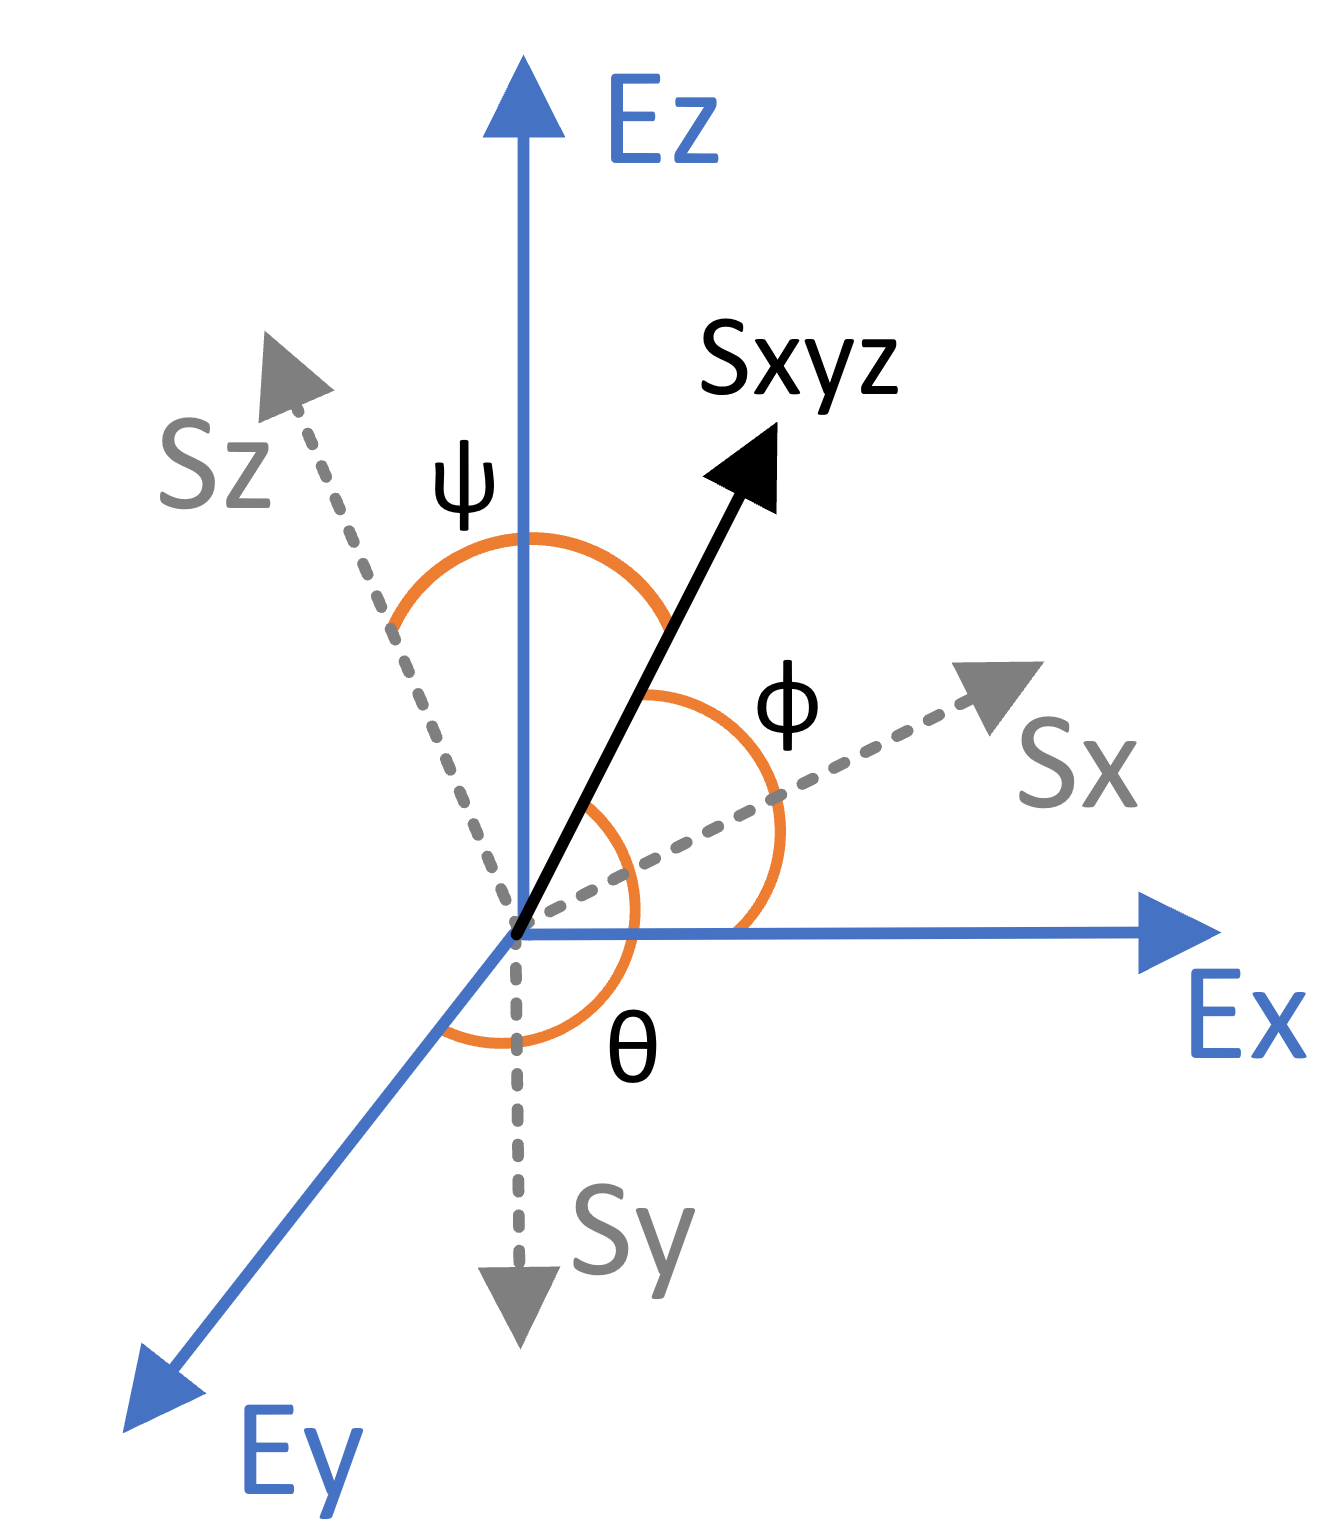
\includegraphics[width=\textwidth]{TESIS/imagenes/chap05/frame-translation.PNG}
  \caption{La orientación del marco E se logra mediante una rotación, desde la alineación con el marco S, de un ángulo de ($\phi,\theta ,\psi$) = (roll,yaw,pitch) alrededor del eje $S_{xyz}$.}
  \label{fig:sfig2}
\end{subfigure}
\caption{Tres ejes de coordenadas dimensionales del IMU. Sistemas de coordenadas de referencia del Sensor ($S_XS_YS_Z$) e Inercial ($E_XE_YE_Z$), traslación del vector en S hacia E, mediante rotación de ángulos. }
\label{fig:sensor-frame}
\end{figure}

% Como 2.1.Presentar Madwick
\section{Algoritmo Filtro de Orientación} \label{impl:orientation-filter}

Para estimar la orientación de los dispositivos respecto a un sistema de referencia inercial, se decide aplicar la técnica de \textit{gradiente descendiente optimizado y derivado analíticamente} sugerida por S. Madgwick -toma de decisión en \nameref{section:filter_orientation}-, descripta en la figura FIG. \ref{FIG: madgwick} tomada de \cite{Madgwick}. El método, presenta grandes ventajas, logrando excelentes resultados en la estimación y siendo computacionalmente eficiente.

\begin{figure}[H]
    \centering
    \resizebox{\textwidth}{!}{
    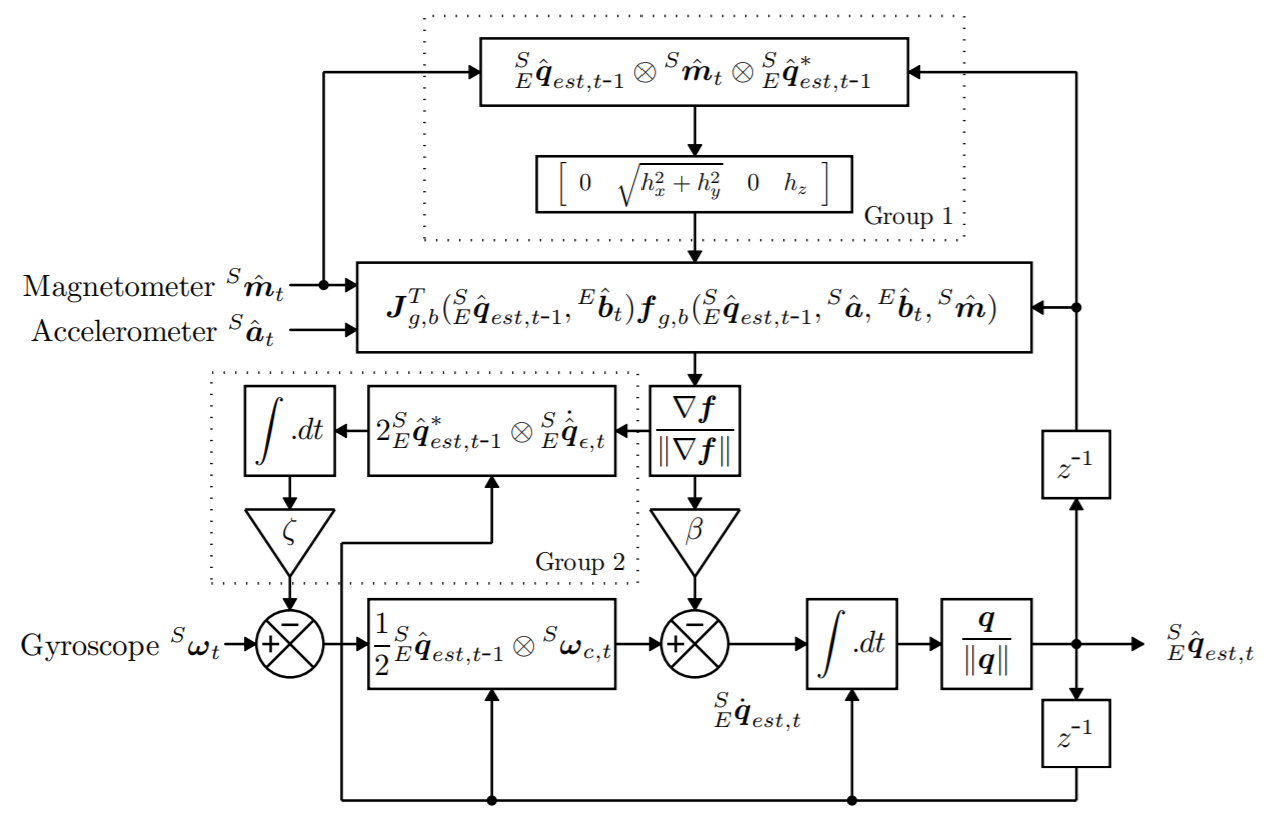
\includegraphics{TESIS/imagenes/img/madgwick.png}}
    \caption{Filtro de orientación con distorsión magnética. Extraído de S. Madgwick \cite{Madgwick}.}
    \label{FIG:madgwick}
\end{figure}

En primer lugar, se realizó un relevamiento respecto a implementaciones de código abierto del algoritmo en el mismo lenguaje de desarrollo que PARKIBIP -de forma que se pueda reutilizar directamente-. No obstante, no se encontró una implementación oficial o alternativa en el lenguaje JAVA, y  si se obtuvo un ejemplo en el lenguaje \textit{Matlab} que sirvió como guía en el desarrollo y pruebas funcionales de PARKIBIP.

Por lo tanto, fue implementado en Android -JAVA- el flujo descripto en la figura Fig. \ref{FIG:madgwick} combinando los datos sensados por el acelerómetro, giroscopio y magnetómetro del dispositivo IMU.

%Hablar de la representacion y el resultado de quaternion
Mencionado en las secciones \nameref{API-algoritmos} y \nameref{section:coordenadas}, existen varias formas de representar la información de orientación de un cuerpo, como por ejemplo los ángulos de Euler o los cuaterniones. Un cuaternión es un número complejo de cuatro dimensiones que se puede utilizar para representar la orientación de un cuerpo o un marco de coordenadas en un espacio tridimensional. Si bien son menos intuitivos que los ángulos de Euler y las matemáticas pueden ser un poco más complejas, presentan ciertas ventajas -entre ellas, no padece ``Gimbal lock'', que impide medir la orientación cuando el ángulo de inclinación se acerca a los +/- 90 grados-, y por lo tanto son empleados en la implementación de PARKIBIP.

Es crucial identificar adecuadamente los marcos de referencias y cómo los mismos son interpretados para obtener resultados esperados. Así, se utilizó un sistema de notación de superíndices y subíndices adoptado en \cite{1987Merat}, para denotar los marcos relativos de orientaciones y vectores. Un subíndice denota el marco que se está describiendo y un superíndice denota el marco al que se hace referencia. Por ejemplo, \textbf{$q_{B}^{A}$} describe la orientación del marco B relativo al marco A.

Como se puede apreciar en el modelo \ref{FIG:madgwick}, las observaciones acelerómetro, giroscopio y magnetómetro en el sistema de coordenadas del sensor, actúan como entrada al algoritmo numérico. A partir de dichos datos y el estado del cuaternión previo, se computa la orientación completa del sensor respecto al marco de referencia inercial Tierra. 

\begin{table}[H] 
\caption{Descripción, notación y tipo -entrada o salida- de los parámetros empleados por el algoritmo filtro de orientación.}
\centering
\begin{tabular}{ |c|c|c| } 
 \hline
 \textbf{Descripción} & \textbf{Parámetro} & \textbf{Notación} \\ \hline
 Magnetómetro en el marco del sensor  instante t & Entrada & $m_{t}^{s}$    \\ \hline
 Acelerómetro en el marco del sensor  instante t & Entrada & $a_{t}^{s}$  \\ \hline
 Giroscopio en el marco del sensor instante t & Entrada & $g_{t}^{s}$   \\ \hline
 Orientación de la Tierra relativa al sensor & Salida & $_{E}^{S}\hat{q}_{est,t}$  \\ 
 \hline
\end{tabular}
\end{table}

Finalmente, con la estimación de la orientación completa, es posible rotar un vector de un marco de referencia a otro, particularmente las observaciones tridimensionales sensadas por el IMU. Logrando de esta manera, estandarizar los concepto para un posterior análisis. Un posible procedimiento de rotación de un vector en el marco del Sensor a uno inercial -empleando propiedades particulares de cuaterniones, e.g. el cuaternión conjugado es el inverso de los marcos $q_{S}^{E} = (q_{E}^{S})^{-1}$- es:

\begin{align*}
    v_E&=q_{S}^{E}\cdot v_S \cdot q_{E}^{S}\\
    V_S&: \text{vector en el marco del Sensor}\\
    V_T&: \text{vector en el marco inercial}
\end{align*}

% Como 2.2 Presentar Algoritmo  Zero velocity. Como detecta las fases?

\section{Extracción de la aceleración física del sensor}

En general, las estimaciones de posición y velocidad basadas en acelerómetros de sensores de bajo costo son muy malas e inutilizables. Esto se debe a que la orientación del sensor debe conocerse con un alto grado de precisión para que las mediciones de gravedad se puedan distinguir de la aceleración física del sensor. Ya mencionado, pequeños errores en la estimación de la orientación producirán errores extremadamente altos en la aceleración medida, lo que se traduce en errores aún mayores en las estimaciones de velocidad y posición. Aunque en PARKIBIP el calculo de la posición y velocidad no dependerán únicamente del acelerómetro para mejorar su eficacia -también del giroscopio y magnetómetro-; es crucial eliminar la aceleración gravitatoria incluida en la aceleración sensada.

Entonces, para convertir la medición del acelerómetro en la aceleración física real del IMU -o aceleración del usuario-, es importante comprender exactamente lo que mide éste sensor. En este sentido, el acelerómetro mide tanto la aceleración física del sensor como la contribución de las fuerzas normales que evitan que el acelerómetro acelere hacia el centro de la Tierra. Para medir solamente las componentes de aceleración que son causadas por la aceleración física, las fuerzas normales debe ser removidas. Es decir:

\noindent Sea $am_{S}$ la aceleración del movimiento sensada en el marco del Sensor, $au_{E}$ es la aceleración real del dispositivo en el cuerpo -del usuario-, $g_{E}$ el vector de componentes gravitatorias en el marco inercial, y $R_E^S$ es la matriz de rotación desde el marco inercial a el marco del Sensor:

\[
    am_{S} = au_{S} - R_E^S \cdot \vec{g}, \quad \vec{g} =   \begin{pmatrix}
      0\\
      0\\ 
      g
\end{pmatrix} 
\]  
\noindent Conforme a eliminar las componentes gravitatorias de la medición de aceleración y obtener la aceleración del usuario, se deduce que:

\begin{equation*}
     au_{S} = am_{S} + R_E^S \cdot \vec{g} 
\end{equation*}

\noindent Obteniendo $au_{E}$, la aceleración del movimiento del usuario en el sistema de coordenadas inerciales:
\begin{equation*}
    au_{E} = R_S^E \cdot am_{S} + \vec{g}
\end{equation*}  
    
\noindent Cabe resaltar que, \underline{la matriz de rotación ($R_S^E$)} resulta de una transformación del cuaternión calculado con el algoritmo filtro de orientación ($q_{E}^{S}$) \nameref{impl:orientation-filter}. 
Alternativamente, se podría emplear el producto de cuaterniones para transformar un vector desde un marco a otro de referencias:

\begin{equation*}
    au_{E} = q_{S}^{E}\cdot am_{S} \cdot q_{E}^{S}  + \vec{g}
\end{equation*}

Finalmente, se realiza la conversión desde unidades gravitacionales del acelerómetro (fuerza gravitacional g) a  $m/s^2$, empleando el coeficiente o factor de escala $g$. Esto habilita a, escalar los datos en el \gls{SI}, como también a disminuir la perdida de precisión derivada de la aritmética computacional. 

\section{Algoritmo de Detección de Velocidad Cero PARKIBIP}
\label{zero-velocity-algorithm}

Durante la marcha de una persona, sus pies se encuentran periódicamente en una fase estacionaria, en la que todo el pie se halla en contacto con el suelo y el cuerpo se desplaza hacia adelante girando rígidamente la extremidad inferior sobre la articulación del tobillo. Dicha fase del ciclo de la marcha, es conocida por estacionaria o en inglés Stance. En contraposición, se encuentra la fase de vuelo o Swing. Asimismo, el ciclo Stance-Swing puede ser fragmentado conforme a aumentar la granularidad en dos nuevas fases, golpe de talón o HS (siglas en inglés, Heel Strike) y el despegue de los dedos del pie o TO (siglas en inglés, Toe Off). Frente a este problema, se emplea el algoritmo de deteccion de velocidad cero (ZVD, por sus sigas en inglés). Las figuras Fig. \ref{fig:gait-phases} y Fig. \ref{FIG: ciclo} permiten ilustrar estos conceptos.

A su vez, los sistemas de navegación inercial basados en sensores de bajo costo padecen de errores de propagación asociados a la estimación de sus parámetros espacio-temporales -como ser la posición, que su error crece proporcionalmente al cubo del tiempo de operación del sistema-. Este problema intrínseco puede reducirse mediante la aplicación de un algoritmo de actualización de velocidad cero (ZVU, siglas en inglés).

Por consiguiente, en PARKIBIP, un algoritmo matemático de detección de velocidad cero tiene los siguientes propósitos:
\begin{itemize}
    \item Identificar eficazmente los  4 eventos de fases de la marcha -HS, Stance, TO y Swing- a partir de un metodo de ZVD.
    \item Aplicar adecuadamente la técnica ZVU -basado en ZVD- para reducir el crecimiento de los errores en el sistema de navegación inercial.
\end{itemize}

Detectado un evento de velocidad cero, el sistema aplica actualizaciones fuertes (en ingles, hard), es decir, cuando el sistema impone una actualización de velocidad cero los parámetros espacio-temporales se ven automáticamente reajustados. Por ejemplo, la velocidad instantánea se establece en cero, la posición y la orientación se vuelven a inicializar.

\noindent Previo a que se utilicen las mencionadas compensaciones de velocidad cero, se requiere la identificación de los instantes de tiempo en los cuales los dispositivos inerciales se encuentran estacionarios. A continuación, se define una adaptación del problema en cuestión que soporte la ejecución en tiempo real del algoritmo, y se mencionan los métodos de detección de velocidad cero desarrollados e integrados al diseño de la solución de PARKIBIP.

Matemáticamente, se formaliza el problema de detección estacionaria como un problema de prueba de hipótesis binarias, donde el algoritmo puede elegir entre las dos hipótesis $H_0$ y $H_1$, tal que:

\[\left\{ 
    \begin{matrix*}[l]
     H_0: \text{IMU en movimiento (hipótesis nula)}\\
     H_1: \text{IMU en Stance (hipótesis alternativa)}
    \end{matrix*}
\right. \]

\noindent Sea $y_k \in R^6$ el vector compuesto por las componentes tridimensionales aceleración ($y_k^a \in R^3$) y velocidad angular ($y_k^w \in R^3$), medidas por el acelerómetro y giroscopio respectivamente en el instante $k$:

\[
     \vec{y_k} = \begin{bmatrix*}[l]
     \vec{y_k^a}\\
     \vec{y_k^w}
    \end{bmatrix*}
\]

\noindent Sea la ventana de tiempo \textbf{W} -WINDOWS-SIZE- pre-establecida y \textbf{configurable en PARKIBIP}, representando el número de observaciones incluidas en la decisión estadística. El objetivo del detector es determinar si en los instantes de tiempo n y n+W-1 el IMU está en movimiento o estacionario, a partir de una secuencia de medición $z_n$: 
\begin{equation*}
    \vec{z_n} = {\vec{y_k}}_{k=n}^{n+W-1}
\end{equation*}

\noindent Luego, la decisión estadística se toma de tal manera que la probabilidad de decidir si el IMU está estacionario cuando ésto no ocurre debe mantenerse baja. Para ello, se emplea el teorema de Neyman-Pearson (NP), que indica cómo elegir entre las dos hipótesis para maximizar la probabilidad de acierto $P_D = Pr\{H_1|H_1\}$ (i.e. la probabilidad de decidir la hipótesis $H_1$ cuando la misma es cierta) dado un $P_{FA} = Pr\{H_1|H_0\}$ (i.e. la probabilidad de decidir la hipótesis $H_1$ cuando la hipótesis $H_0$ es verdadera).

De esta manera, se decidió desarrollar e integrar a la solución dos alternativas de algoritmos numéricos de detección de velocidad cero, que luego favorecerán a evaluar el desempeño de cada uno \label{base-detectors}:

\begin{enumerate}
    \item \textbf{Acceleration Moving Variance Detector (MVD)}. Se basa únicamente en los datos del acelerómetro y la decisión de aceptar $H_1$ se deduce de la siguiente manera:
   \[\left\{ 
     \begin{matrix*}[l]
     T_v(z_n^a) = \frac{1}{W} \sum_{k=n}^{n+W-1}\lVert y_k^a - \overline{y_n^a} \rVert^2 < \gamma_v\\\\
     \overline{y_n^a} = \frac{1}{W}\sum_{k=n}^{n+W-1}y_k^a\\\\
     \gamma_v: \text{umbral o threshold de aceptación}
    \end{matrix*}
    \right. \]
    
    \item \textbf{
Generalized Likelihood Ratio Test (GLRT)}. Adquiere mayor información integrando al análisis, además de las aceleraciones observadas; las señales del giroscopio -velocidades angulares-. La aceptación de $H_1$ viene dada por la formula:
\[\left\{ 
     \begin{matrix*}[l]
     T(z_n) = \frac{1}{W} \sum_{k=n}^{n+W-1}(\frac{1}{\theta_a^2}\lVert y_k^a -g \frac{\overline{y_n^a}}{\lVert \overline{y_n^a}\rVert} \rVert^2 + \frac{1}{\theta_w^2}\lVert y_k^w\rVert^2) < \gamma\\\\
     \overline{y_n^a} = \frac{1}{W}\sum_{k=n}^{n+W-1}y_k^a\\\\
     \overline{y_n^w} = \frac{1}{W}\sum_{k=n}^{n+W-1}y_k^w\\\\
     \theta_a^2:\text{varianza del ruido del acelerómetro}\\\\
     \theta_w^2: \text{varianza del ruido del giroscopio}\\\\
     \gamma: \text{umbral o threshold de aceptación}
    \end{matrix*}
    \right. \]

\end{enumerate}

Por lo tanto, se desarrolló en el lenguaje de programación JAVA, para Android, una clase abstracta -no instanciable- denominada ``ZeroVelocityDetector''. Dicha clase define la estructura y las propiedades que compartirán las subclases derivadas que implementen a la clase abstracta, mediante los conceptos jerarquía y herencia. Luego, fueron realizadas las dos clases especificas ``GLRatioTestDetector'' y ``MovingVarianceDetector'', las cuales implementan las decisiones estadísticas particulares citadas en \nameref{base-detectors} (e.g. la ejecución del test $ T(z_n) $), y mantienen el comportamiento de la superclase ZeroVelocityDetector (e.g. estructuras de datos, agregar una medición para efectuar un test, gestionar el resultado del test). 

\begin{figure}[H]
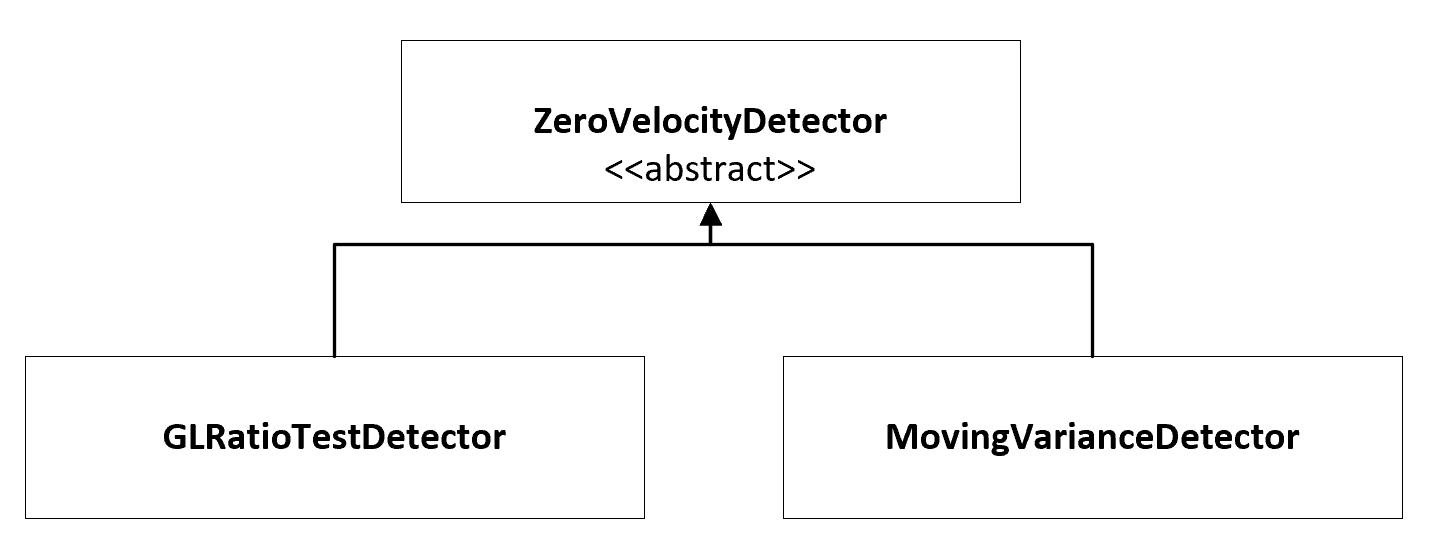
\includegraphics[width=\textwidth]{TESIS/imagenes/chap05/detectors-hierachy.PNG}
\caption{Componentes de deteccion de velocidad cero. Superclase abstracta ZeroVelocityDetector, subclases GLRatioTestDetector y MovingVarianceDetector.}
\label{FIG: Arquitectura2}
\end{figure}

\noindent Así pues, se emplearon dos estructuras de datos auxiliares. Primero, una cola FIFO del tamaño $W$ implementada con la estructura de datos LinkedList, destinada a almacenar las mediciones recepcionadas por el detector. Segundo, un arreglo de estados booleanos del mismo tamaño, que permite almacenar e iterar sobre los resultados de los tests estadísticos.

\noindent Cuando el ZVD detecta un nuevo evento de medición, en orden de precedencia ocurren los siguientes pasos dentro del detector:
\begin{enumerate}
    \item El sistema almacena la nueva medición en la cola FIFO
    \item Chequea si la cantidad de elementos de la cola es igual al tamaño de la ventana $W$ (caso base de primer procesamiento). Esto es, recopila los datos necesarios para el primer procesamiento, luego, a medida que llegan mediciones se agregan y se remueven elementos -el número de elementos es W-
    \item En caso de que la cola tenga $W$ observaciones, el detector procede a efectuar el test estadístico según el algoritmo ZVD seleccionado.
    \item Posterior, el resultado del test es almacenado en el arreglo de resultados de tal forma que:
    \begin{itemize}
        \item Si el test es positivo ($H_1$, es estacionario), todos los elementos del arreglo booleano se convierten en 1.
        \item Se obtiene y remueve el primer elemento del arreglo -primer test almacenado y actualizado W-1 veces dentro de la ventana W-.
        \item Se desplazan un lugar hacia la izquierda los restantes tests del arreglo (en inglés, left shift), y el último elemento $W-1$ es inicializado en 0 (i.e. $H_0$ o hipótesis nula).
    \end{itemize}
    \item Se despacha el resultado del test obtenido al listener u oyente del detector (en general, un analizador de datos), previamente establecido.
    \item Finalizado el procesamiento, en caso de que la cola de mediciones posea $W$ elementos, se remueve la primer medición y se continua iterando.
\end{enumerate}

Con el fin de clarificar las etapas mencionadas, se propone el pseudocódigo \nameref{pseudo-code-detectors}, sin embargo, no se refinan los metodos auxiliares empleados (e.g. makeTest, pushStatisticalTest).

\begin{algorithm}[H]
\caption{Pseudocódigo Zero Velocity Detector} \label{pseudo-code-detectors}
\begin{algorithmic}[1]
   \State Queue$<$MeasurementModel$>$ measures;
   \State Array$<$Boolean$>$ zupdtValues;
    \State W $\gets$  windowSize;
    \State setupParameters();
    \Statex
     \Function{updateDetector}{data}
        \State addQueue(measures,data);
    
        \If{sizeQueue(measures) == W} \Comment{PB. Espera por una ventana }

            \State boolean currentTest $\gets$  makeTest(); \Comment{Ejec. del test particular}

            \State int zValue $\gets$  pushStatisticalTest(currentTest); 
               
            \State removeQueue(measures);
            \State dispatchEventDetected(zValue); 
        \EndIf

    \EndFunction
    \Statex
     \Function{pushStatisticalTest}{test}
    
        \Comment{Actualizar la secuencia}
        \If{isH1 (test)} 
            \State setOnes(zupdtValues); \Comment{Establecer ventana en unos}
        \EndIf
        \Comment{shift data}
        \State z $\gets$ zupdtValues[0];
        \Comment{Shift 1 elemento a la izquierda}
        \ForAll{zupdtValues - 1}
           \State zupdtValues[i] $\gets$ zupdtValues[i+1];
        \EndFor
        \Comment{Próximo test en 0}
        \State zupdtValues[windowsSize-1] = 0;
        \Return{z};
   \EndFunction
\end{algorithmic}
\end{algorithm}

% Como 2.3 Presentar Algoritmo  Kalman Filter y Parámetros espacio-temporales
\section{Algoritmo Filtro de Kalman PARKIBIP}

A modo introductorio, en el capitulo \nameref{chap:project}, apartado \nameref{section:kalman-filter}, se presentó un algoritmo óptimo de estimación denominado filtro de Kalman; el cual sirve para poder identificar el estado oculto -no medible- de un sistema dinámico lineal que está sometido a ruido blanco Gausseano -cuya función de densidad responde a una distribución normal-. Es decir, permite hallar la mejor estimación de variables de interés no medibles (e.g. velocidad), a partir de la combinación de variables indirectas que son medibles (e.g. aceleración). Asimismo, con la finalidad de introducir a la temática se mencionaron brevemente algunas de sus aplicaciones, siendo en ciertos casos, el problema de estimar la posición de un sistema de navegación de un automóvil en movimiento similar al modelo empleado en PARKIBIP.

Análogo a lo sucedido con la estimación de la orientación en \nameref{impl:orientation-filter}, no se encontró una librería de código abierto que se adecue al contexto de PARKIBIP, y por consiguiente pueda ser reutilizada. 

Por lo tanto, se implementó un filtro de Kalman avanzado y multidimensional, en notación matricial. El propósito de dicho filtro es estimar las variables indirectas posición, velocidad y ángulos de Euler en cada instante de tiempo, a partir de las variables acelerómetro, giroscopio y magnetómetro sensadas por el dispositivo IMU. Para llevar adelante esta tarea, se requieren conocimientos y funciones avanzadas en álgebra lineal (e.g. operaciones matriciales) y física (e.g. leyes mecánicas, rotaciones y traslaciones). Todas las operaciones auxiliares requeridas fueron implementadas en la API de algoritmos en \nameref{API-algoritmos}.

El filtro de Kalman es un método numérico Predictor-Corrector, explicito de un solo paso; es decir depende únicamente de la estimación del estado previo ($x_{k-1}$) para lograr predecir el siguiente estado ($x_{k}$). El procedimiento Predictor-Corrector comienza mediante una primera predicción de los valores de las variables -resultantes de la extrapolación de una función ajustada (e.g. leyes mecánicas)-, luego, el corrector, refina la aproximación inicial utilizando el valor predicho de la función y una función objetivo que minimiza el error cuadrático medio del problema en cuestión.

Dada la complejidad del análisis, se deducen las ecuaciones físico-matemáticas y la metodologıa numérica empleada, así como un pseudo-código de la resolución de Kalman Filter con actualizaciones de cero velocidad.

\noindent Sea el \textbf{vector de estado} $\boldsymbol{x_k}$ en la iteración $\boldsymbol{k}$, dado por:

\[\left\{ 
            \begin{matrix*}[l]
            x_{k} = [P_k,V_k,O_k] = [position, velocity, orientation]\\
            P_k = (p_0,p_1,p_2),  p_i \in R \\
            V_k = (v_0,v_1,v_2), v_i \in R \\
            O_k = (roll,pitch,yaw),  o_i \in R
            \end{matrix*}
\right. \]

\noindent Previo a introducir el procedimiento del algoritmo, es imprescindible presentar los \textbf{Coeficientes} que intervienen en el formulamiento del filtro de Kalman y los roles que cumplen:

\begin{align*}
    F &= \text{Matriz Predicción o Transición} \\
    B &= \text{Matriz de Control} \\
    u &= \text{Vector de Control} \\
    P &= \text{Matriz de error de Covarianza de Estado} \\
    H &= \text{Matriz de Medición o relación entre mediciones y el vector de estado} \\
    R &= \text{Matriz de error de Covarianza Ruido de Medición} \\
    Q &= \text{Matriz de error de Covarianza Ruido del proceso} \\
\end{align*}

\noindent Aplicando las ecuaciones dadas por las \textbf{leyes mecánicas del movimiento} tanto para la posición como para la velocidad en función de la aceleración -medida por el sensor inercial- y el tiempo, se obtiene la siguiente formulación:

\[ 
x_k =\begin{bmatrix}
P_k\\
V_k
\end{bmatrix} = \begin{bmatrix}
P_{k-1} + V_{k-1}\Delta t +\frac{\Delta t^2}{2} \\
V_{k-1} + acc\Delta t
\end{bmatrix}
\]  


\noindent Reordenando los términos en función del vector de estados:
\begin{equation}
    x_k = \begin{pmatrix}
              1 & \Delta t\\ 
                 0 & 1
            \end{pmatrix} X_{k-1} +
            \begin{pmatrix}
  \frac{\Delta t^2}{2}\\ 
  \Delta t
\end{pmatrix} acc
\end{equation}  

\begin{equation}
     x_k = F X_{k-1} + B u
\end{equation}

\noindent Definiendo los cambios de variables, hallamos los valores \textbf{F} = $\begin{pmatrix}
              1 & \Delta t\\ 
                 0 & 1
            \end{pmatrix}$, \textbf{B} =$\begin{pmatrix}
  \frac{\Delta t^2}{2}\\ 
  \Delta t
\end{pmatrix}$ y $\boldsymbol{u_{k-1}}$ = acc. 

Finalmente, Se logra obtener un método iterativo para predecir las ecuaciones de navegación o transición de estados, que puede ejecutarse en tiempo real a medida que se recopilan los datos de medición.

\noindent Entonces, para el paso (i), se llama $\hat{x_{k}}$ y $\hat{P_k}$ las variables estimadas en la predicción y sus ecuaciones vienen dadas por:
\[ (i) \boldsymbol{Predicci\Acute{o}n}\left\{ 
            \begin{matrix}
            \hat{x_{k}} = F X_{k-1} + B u_{k-1} + w_{k-1} \\
            \hat{P_k} = FP_{k-1}F^t + Q\\
             u_{k-1}=(accX,accY,accZ)
            \end{matrix}
\right. \]

\noindent Luego, en (ii), se ejecuta la actualización de los valores estimados mediante la aplicación del factor de ganancia de Kalman. Primero, calcula el factor de ganancia $K$, corrige el estado con la medición, actualiza la matriz de Covarianza. Esto es:
\[ (ii) \boldsymbol{Correcci\Acute{o}n}\left\{ 
            \begin{matrix}
            K_k = \frac{\hat{P_k}H^t}{H.\hat{P_k}H^t + R}\\
            y_k = H\hat{x_{k}} +v_k\\
            x_{k} =  \hat{x_{k}} + K_k y_k\\
            P_k = (I -K_k.H)\hat{P_k}
            \end{matrix}
\right. \]

%TODO: no hay referencia a esta imagen 
\begin{figure}[H]
    \centering
    \captionsetup{justification=centering}
    \resizebox{\textwidth}{!}{
    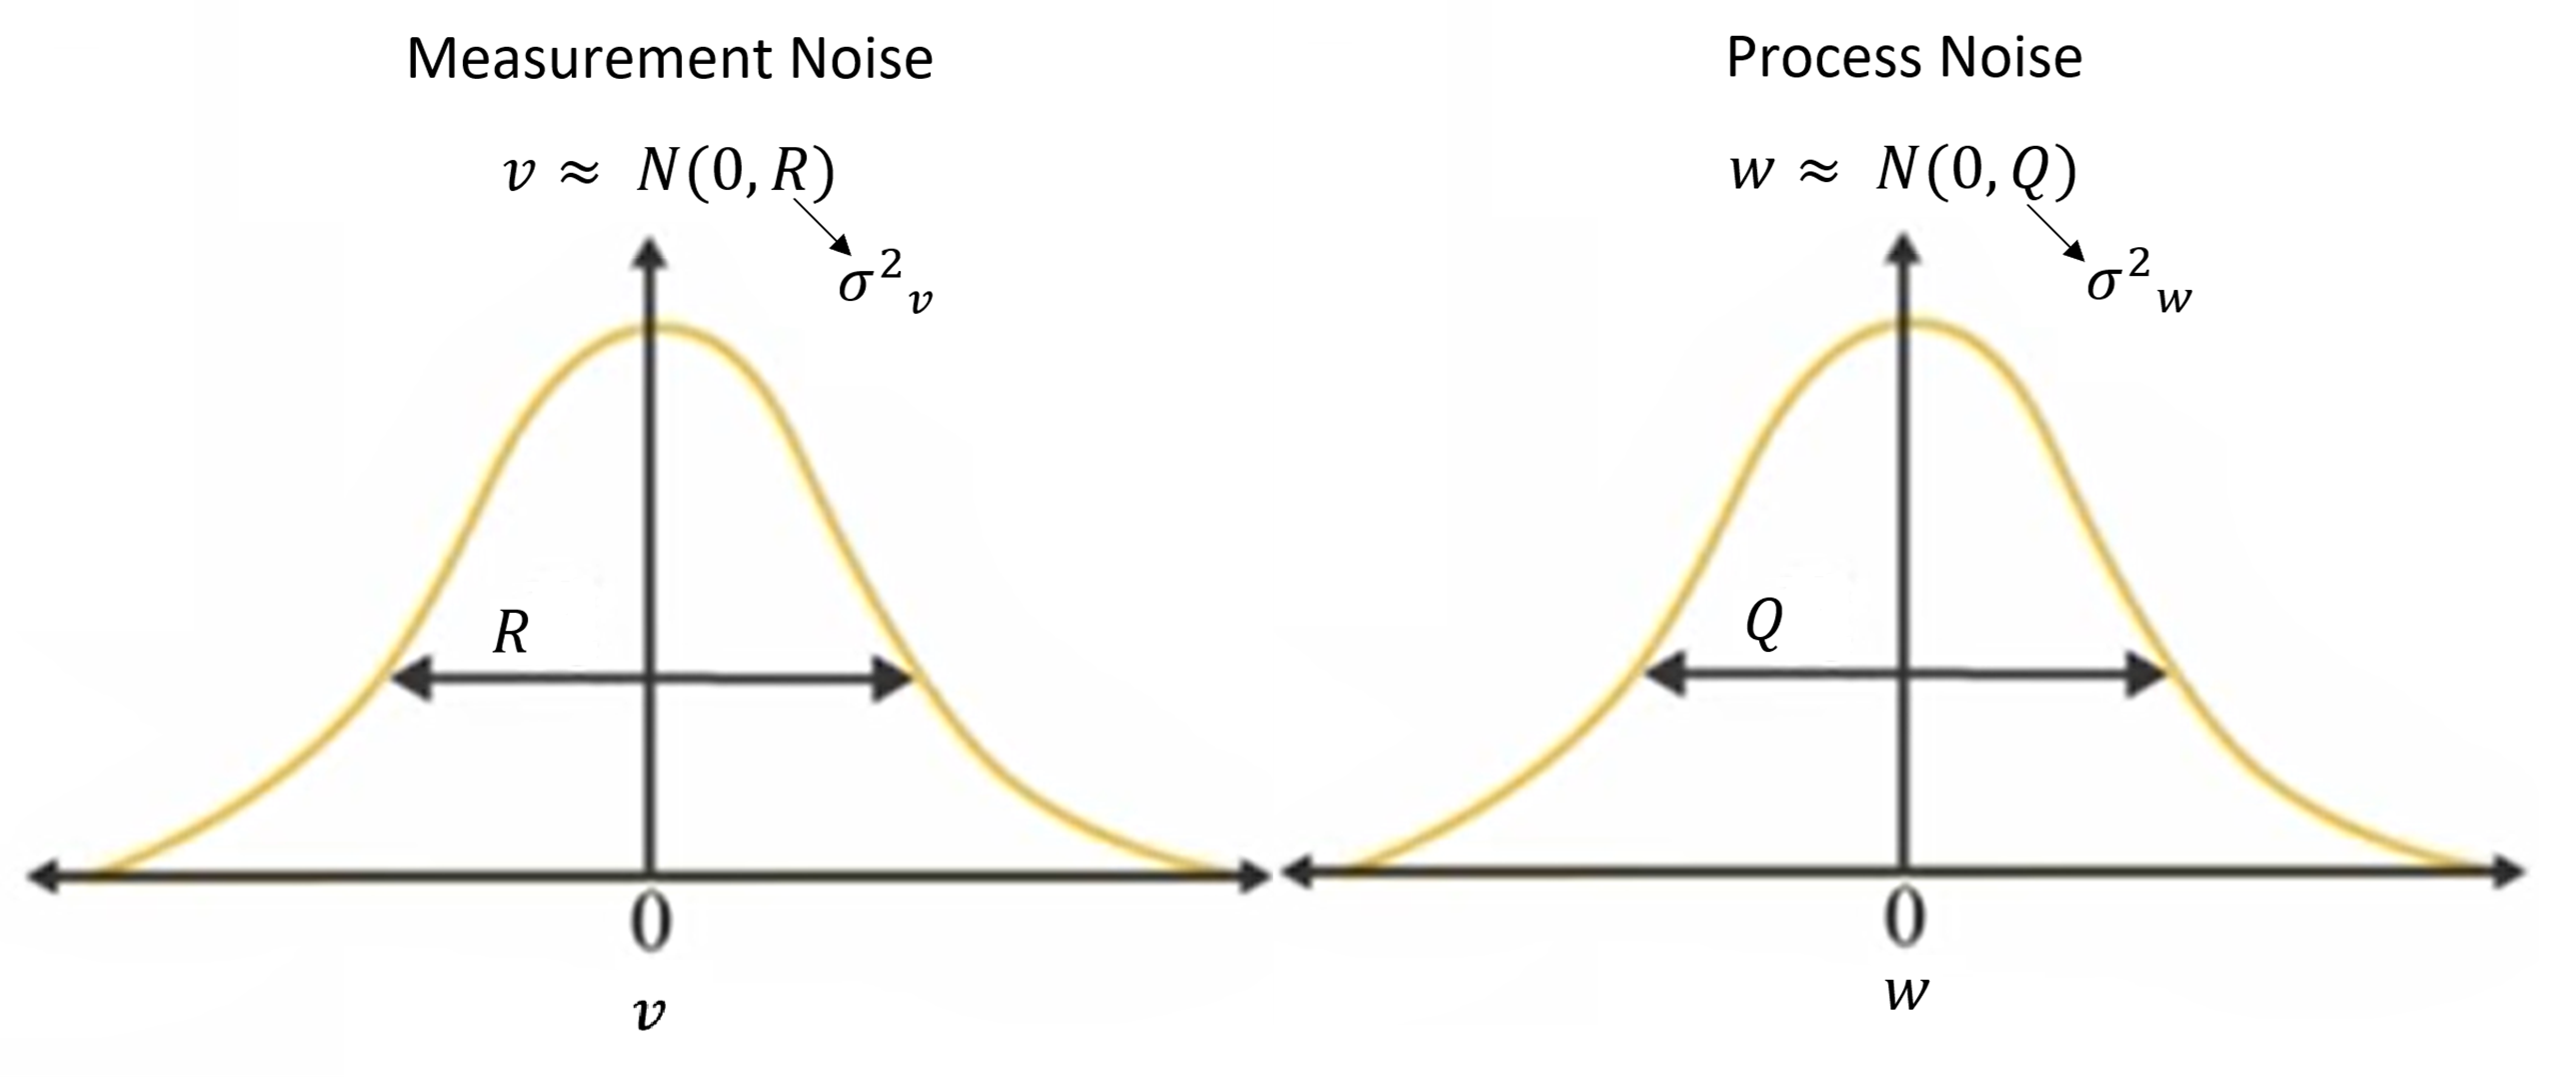
\includegraphics{TESIS/imagenes/chap05/kalman-noises.PNG}}
    \caption{Distribuciones supuestas para los vectores de ruido estadísticos de Medición $v_k$ y de Proceso $w_k$.}
    \label{FIG: madgwick}
\end{figure}

El sistema de ecuaciones debe contemplar los desvíos relacionados a los distintos ruidos estadísticos. Para esto, se asume que los vectores $v_k$ y $w_k$ de ruido de medición y proceso poseen una distribución gaussiana de media cero y covarianzas R y Q respectivamente. Las matrices Q y R en general se emplean como parámetros de ajuste para obtener el rendimiento deseado.

Una particularidad crucial del modelo empleado, es la integración del método Zero Velocity al filtro de Kalman. Esta tarea permite \underline{compensar la velocidad} en la etapa de corrección (ii), llevando su valor a Cero en caso de que el algoritmo Zero Velocity Detector identifique un momento estacionario. Así, se reducen considerablemente los desvíos incrementales debido al error acumulativo de integración respecto al tiempo.

\begin{algorithm}[H] 
\caption{Pseudocódigo de Kalman Filter con compensacion Zero Velocity} \label{pseudo-code-kf}
\begin{algorithmic}[1]
    \Function{initKalmanFilterZUpdtate}{A}  
        \State initFilters();
        \State initVectors();
    \EndFunction
    \Statex
     \Function{runKalmanFilterZUpdtate}{$measure_k, zValue_k$}
        \Statex
        \Comment{\textbf{Prediction with previous $x_h$}}
        \State xhat $\gets$ NavigationEquations($measure_k, x_h$);
        \Statex
         \Comment{\textbf{Compute F and G}}
        \State stateMatrix($measure_k$); 
        \Statex
        \Comment{\textbf{Predict state covariance matrix $P=F*P*F'+G*Q*G'$;}}
        \State P$\gets$F.multiply(P).multiply(F.transpose()).add(G.multiply(Q).multiply(G.transpose())); 
        
        \Comment{\textbf{Check covariance matrix P is symmetric}}
        \State P $\gets$ P.add(P.transpose()).scalarMultiply(0.5d);
        
        \Statex
        \Comment{\textbf{Check if a zero velocity update should be done}}
        \If{$zValue == true$}

                \Statex 
                \Comment{\textbf{K=(P*H')/(H*P*H'+R); s = H*P*H'+R, solve s'.k'=H.P'}}
                \State RealMatrix s $\gets$ H.multiply(P).multiply(H.transpose()).add(R);
                \State RealMatrix b $\gets$ H.multiply(P.transpose());
                \State RealMatrix K$\gets$new CholeskyDecomposition(s.transpose()).solve(b).transpose();

               \Statex
               \Comment{ \textbf{Innovation z=-x}}
               \State RealVector innovation $\gets$ H.operate(xhat).mapMultiply(-1);

               \Comment{\textbf{Correct xhat using the estimated perturbations}}
               \State RealVector dx $\gets$ K.operate(innovation);
               \State $x_h$ $\gets$ xhat.add(dx);
               
               \Statex \Comment{\textbf{Compensate current orientation}}
               \State compensateOrientation(dx);
               
               \Statex
               \Comment{\textbf{Compensate current covariance matrix P}}
               \State P = Id.subtract(K.multiply(H)).multiply(P);
               
               \Statex
               \Comment{\textbf{Check covariance matrix P is symmetric}}
               \State P $\gets$ P.add(P.transpose()).scalarMultiply(0.5d);

        \Else
            \State $x_h$ $\gets$ xhat; \Comment{\textbf{Update new $x_h$ if not correction is done}}
        \EndIf

    \EndFunction

\end{algorithmic}
\end{algorithm}
 
Para concluir con la exposición de el filtro de Kalman integrado a un detector de cero velocidad, se expone el \textbf{pseudo-código} de la implementación realizada en el lenguaje Java de Android dado por \nameref{pseudo-code-kf}. El filtro se inicializa mediante la función ``initKalmanFilterZUpdate'', luego con la recepción de cada medición se ejecuta la función ``runKalmanFilterZUpdate''.

Los valores empleados para los coeficientes fueron elegidos acorde a la especificación del hardware y para optimizar el funcionamiento de la aplicación. A continuación, se exponen las configuraciones para el ruido de proceso, el ruido de medición y matrices de covarianza de estado inicial Q, R y P. Se supone que las tres matrices son matrices diagonales y todas las configuraciones se definen como desviaciones estándar:

\begin{itemize}
    \item Período de muestreo del sistema:
    \begin{itemize}
        \item Ts [seg]= (1/f), f frecuencia configurable 
    \end{itemize}
    \item Ruido de proceso para modelar el ruido del acelerómetro (eje de coordenadas x, y, z) y otros errores del acelerómetro:
    \begin{itemize}
        \item Ruido de Aceleración[m/$s^2$]: sigmaAcc = $0.5^{2}$
    \end{itemize}
    \item Ruido de proceso para modelar el ruido del giroscopio (eje de coordenadas x, y, z) y otros errores del giroscopio:
    \begin{itemize}
        \item Ruido Angular[rad/s]: sigmaGyro = $(0.5*pi/180)^{2}$ 
    \end{itemize}
    \item Elementos diagonales de la matriz de Covarianza P del estado inicial:
     \begin{itemize}
        \item Varianza de Posición [m]: sigmaP = $(1\cdot10^{-5})^{2}$ 
        \item Varianza de Velocidad [m/s]: sigmaV = $(1\cdot10^{-5})^{2}$
        \item Varianza de Orientación [rad]: sigmaAtt = $(pi/180*0.1)^{2}$
        \item Desviación de Aceleración[m/$s^2$]: sigmaA =$(0.3)^{2}$
        \item Desviación de Velocidad angular [rad/s]: sigmaG = $(0.*pi/180)^{2}$ 
    \end{itemize}
    \item Covarianza de ruido de medición R:
    \begin{itemize}
        \item Desviación de Velocidad sigmaVelR [m/s] =0.01
    \end{itemize}
    
\end{itemize}

El vector de estados se inicializa mediante un \textbf{Procedimiento de Calibración}. El mismo consiste en recopilar las primeras N = 30 observaciones del sistema, computar la media de las variables roll, pitch, yaw; luego establecer el vector de estados. La posición y la velocidad inicial comienza con el valor 0:
\begin{equation*}
    X_{initial}= \begin{pmatrix}
0&0&0&0&0&0& \bar{roll}& \bar{pitch}& \bar{yaw}
\end{pmatrix}
\end{equation*}

Los coeficientes estables del sistema dinámico P (inicial), Q, H, R, fueron establecidos de la siguiente manera:
\begin{equation*}
    P_{initial}  = \begin{pmatrix}
sigmaP&0&0&0&0&0&0&0&0\\    
0&sigmaP&0&0&0&0&0&0&0\\
0&0&sigmaP&0&0&0&0&0&0\\
0&0&0&sigmaV&0&0&0&0&0\\
0&0&0&0&sigmaV&0&0&0&0\\
0&0&0&0&0&sigmaV&0&0&0\\
0&0&0&0&0&0&sigmaAtt&0&0\\
0&0&0&0&0&0&0&sigmaAtt&0\\
0&0&0&0&0&0&0&0&sigmaAtt
\end{pmatrix} 
\end{equation*}
\begin{equation*}
% %//6x6
Q  = \begin{pmatrix}
sigmaAcc&0&0&0&0&0\\    
0&sigmaAcc&0&0&0&0\\
0&0&sigmaAcc&0&0&0\\
0&0&0&sigmaGyro&0&0\\
0&0&0&0&sigmaGyro&0\\
0&0&0&0&0&sigmaGyro
\end{pmatrix}
\end{equation*}

\begin{equation*}
% %//3x9
H  = \begin{pmatrix}
0&0&0&1&0&0&0&0&0\\    
0&0&0&0&1&0&0&0&0\\
0&0&0&0&0&1&0&0&0\\
\end{pmatrix}
\end{equation*}

\begin{equation*}
%% 3*3
R  = \begin{pmatrix}
sigmaVelR&0&0\\
0&sigmaVelR&0\\
0&0&sigmaVelR
\end{pmatrix}
\end{equation*}
% $\in$ $M{9\times9}$

Los restantes valores -P, F, B, u-, mutan según las observaciones recopiladas en cada instante de tiempo y la dinámica del sistema. Se resalta la implementación de un algoritmo iterativo, que reacciona con cada evento de medición.

En orden de precedencia ocurren los siguientes eventos de sistema:
\begin{enumerate}
    \item Recopilación de mediciones: aceleración, velocidad angular, fuerzas magnéticas
    \item Estandarización de unidades inerciales sobre las mediciones
    \item Computo de la orientación instantánea en formato cuaternión -a partir de los datos medidos- mediante filtro eficiente de orientación
    \item Con la orientación adquirida. Rotación a un marco de referencia inercial -tierra-, desde el marco del sensor
    \item Ejecución de algoritmo Zero Velocity Detector
    \item Ejecución del filtro de Kalman con los datos procesados -cuaternión, mediciones, zero velocity-
\end{enumerate}

\newpage

\section{Analizadores de datos} 

Los analizadores de datos son las entidades que tienen por misión procesar los datos crudos que provienen desde los distintos sensores del IMU, utilizando los métodos numéricos ya mencionados (e.g detección de velocidad cero, filtrado de Kalman, entre otros). Son representados en el sistema mediante la clase \textit{DataAnalyzer}. El diseño de clases de esta sección del sistema se puede ver en la figura Fig. \ref{FIG:data-analyzer-class-diagram}. 

\begin{figure}[H]
    \hspace*{-3.0cm}%
    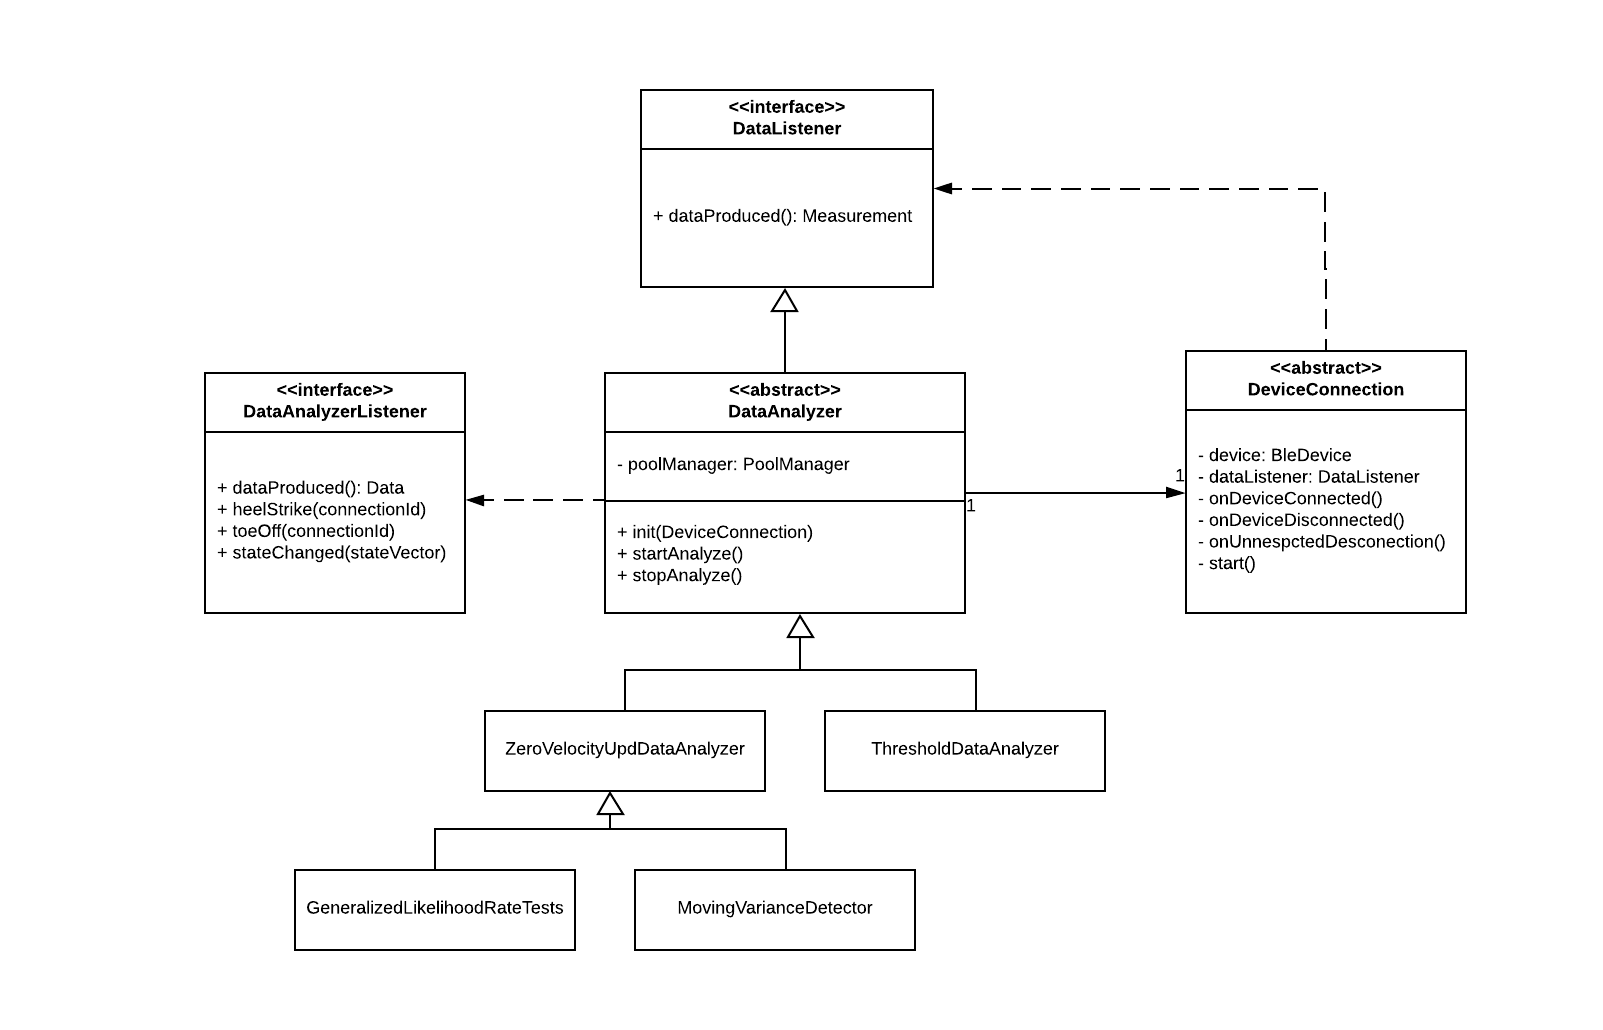
\includegraphics[clip,width=1.3 \columnwidth]{TESIS/imagenes/chap05/data-analyzers-class-diagram.png}    
    \caption{Diagrama de clases del módulo de la aplicación Android en donde se analizan y procesan los datos para detectar eventos relativos a la marcha del paciente.}
    \label{FIG:data-analyzer-class-diagram}
\end{figure}

Tal como se puede apreciar en la figura, el \textit{DataAnalyzer} implementa la interfaz \textit{DataListener}, y así, posee la capacidad de recibir los datos desde una instancia de \textit{DeviceConnection} -entidad que representa una conexión con un dispositivo IMU-. Es decir, cada \textit{DeviceConnection} tiene asociado un \textit{DataAnalyzer}, definido como su \textit{DataListener}. Cuando es invocado el método \textit{startAnalyze()} correspondiente a un analizador, éste le comunica a su \textit{DeviceConnection} que puede comenzar el flujo de datos. La instancia de \textit{DeviceConnection} inicia el envío de datos de medición, representados con el modelo \textit{Measurement}, a través de la interfaz \textit{DataListener}, para que el analizador de datos pueda procesar las mediciones producidas por los sensores. 

Existen diferentes \textit{DataAnalyzers} en la aplicación. Cada uno implementa un método numérico particular para analizar los datos. Durante el diseño se utilizó el concepto de polimorfismo; es decir, el comportamiento de todos los \textit{DataAnalyzers} se encuentra definido en ésta clase abstracta, sin embargo, cada instancia concreta implementa los métodos derivados de forma particular empleando diferentes métodos numéricos. Por ejemplo, \textit{ZeroVelocityUpdateDataAnalyzer} implementa el método de detección de velocidad cero para procesar los datos e identificar los eventos Heel Strike y Toe Off. 

El hecho de utilizar polimorfismo para los analizadores de datos hace que el sistema sea escalable y extensible, ya que implementar un nuevo método para analizar los datos y generar eventos, implica crear únicamente una clase concreta que extienda de la clase \textit{DataAnalyzer}. Además, cada analizador desarrolla un único método de análisis y tiene asignada una única responsabilidad bien definida. Este forma de diseño, contribuye a mejorar la calidad del sistema, haciendo que sea más sencillo realizar pruebas sobre un método de análisis concreto y compararlo con el resto de los métodos; además de incrementar su mantenibilidad. 
Cuando un \textit{DataAnalyzer} detecta eventos u obtiene nuevos datos como resultado, los envía a su \textit{DataAnalyzerListener}. Esta interfaz está definida para ser implementada por la entidad que esté interesada en recibir el resultado del procesamiento, que en la implementación final de PARKIBIP esta entidad es \textit{BiofeedbackModule}. 

\textit{DataAnalyzerListener} es un protocolo definido para ser implementados por las entidades que necesiten observar los resultados de un \textit{DataAnalyzer}. Cuando un analizador de datos detecta cierto evento de la marcha, notifica a su \textit{DataAnalyzerListener}. En PARKIBIP, este protocolo es implementado por \textit{BiofeedbackModule}.

\section{Configuración de algoritmos y parámetros} 

PARKIBIP es también una aplicación experimental. Es decir, si bien el objetivo principal es obtener un sistema que beneficie la marcha de los enfermos de Parkinson; pretende ser, en una primera instancia, una herramienta de investigación que permita encontrar la mejor forma de estimular a un paciente para que su marcha progrese. Por lo tanto, resulta crucial experimentar con los algoritmos desarrollados para estudiar la marcha, poder utilizar un método u otro, configurar éstos métodos numéricos de distintas formas, establecer distintas reglas para definir los estímulos, etc. 

Ante ésta necesidad, se desarrolló un modulo de configuración. Este módulo consta de su propia interfaz gráfica, la cual puede ser encontrada dentro del menú principal de la aplicación. En la figura Fig. \ref{FIG:configuration-class-diagram}, se expone el diagrama de clases correspondiente a la porción del sistema dedicada a la parametrización.

\newpage

\begin{figure}[H]
    \hspace*{-3.5cm}%
    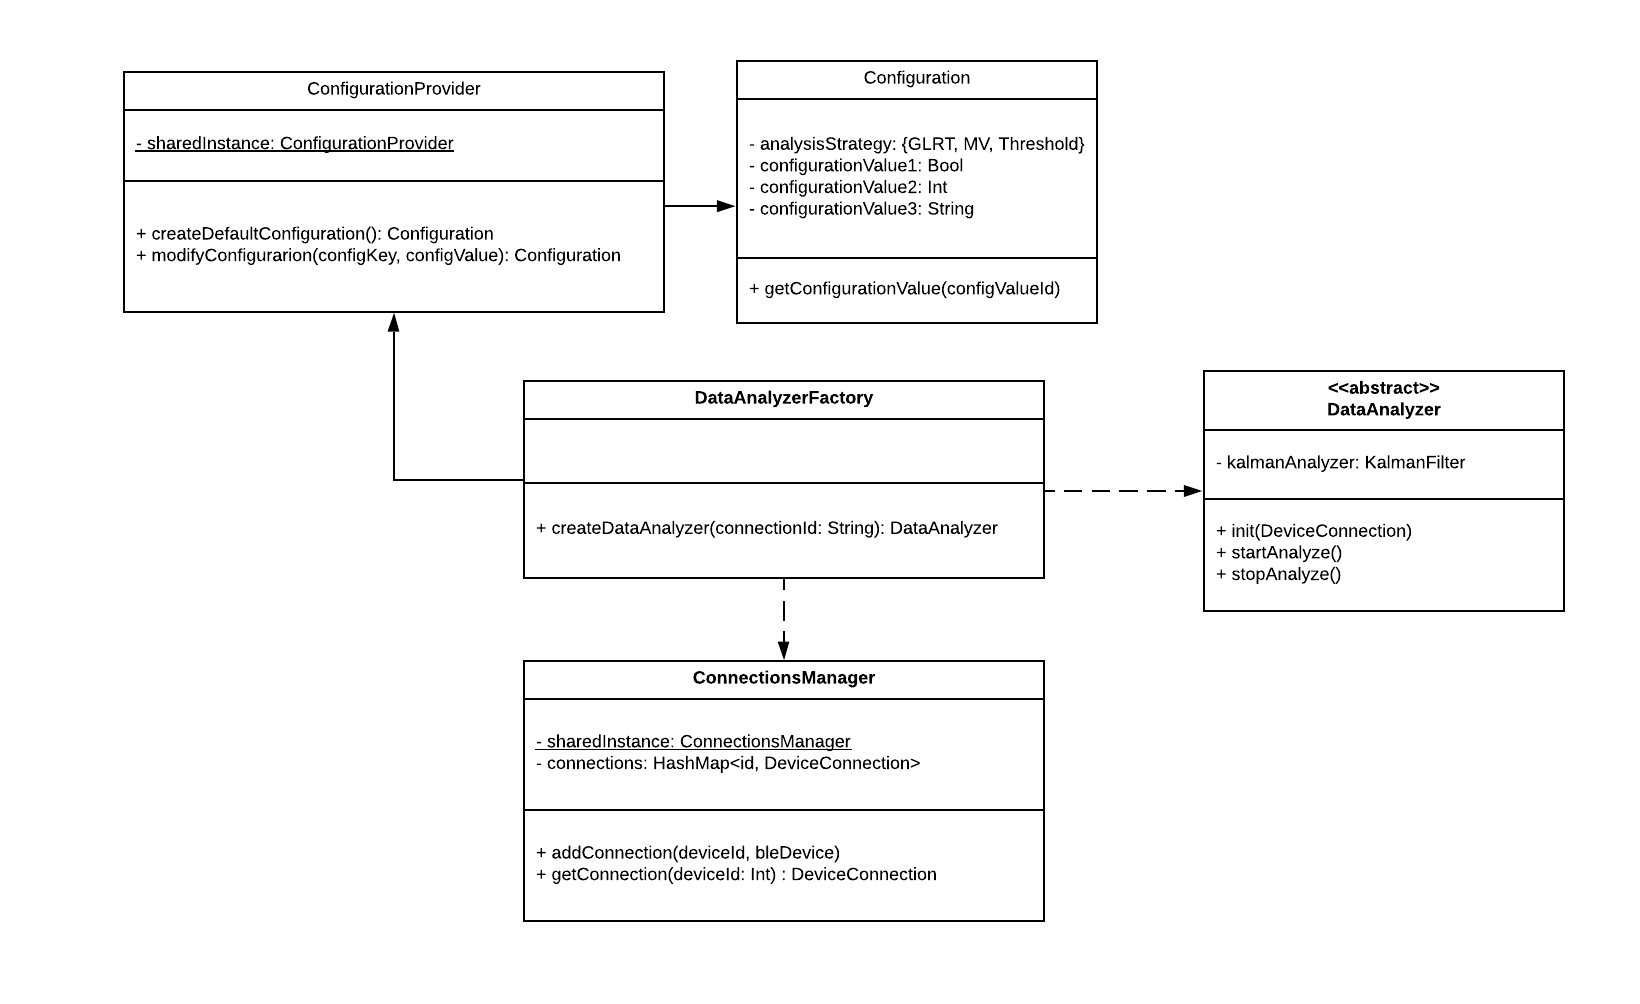
\includegraphics[clip,width=1.4 \columnwidth]{TESIS/imagenes/chap05/configuration-class-diagram.png}    
    \caption{Diagrama de clases del módulo de la aplicación Android donde se administran las distintas configuraciones del sistema}
    \label{FIG:configuration-class-diagram}
\end{figure}

Un estado de configuración está representado por una instancia de la clase \textit{Configuration}. La misma clase, dispone del conjunto de atributos correspondientes a cada uno de los parámetros que pueden ser editados dentro del sistema. A su vez, \textit{ConfigurationProvider} es la clase encargada de manejar éstas configuraciones, por ende, un objeto \textit{Configuration} se mantiene inmutable mientras el proveedor no ejecute una transacción de modificación sobre el mismo. Cuando un valor es modificado a través de la pantalla de Configuraciones de la aplicación, esta \textit{Activity} invoca al proveedor de configuraciones para solicitarle dicho cambio.

\textit{ConfigurationProvider} implementa el patrón de diseño \textit{Singleton}, es decir, una clase para la cual existe una única instancia, y una vez creada se mantiene en memoria durante todo el ciclo de vida de la aplicación Android. Este \textit{Singleton} mantiene una referencia a la instancia de \textit{Configuration} actual, y al ser global, puede ser accedido desde cualquier clase del sistema. 

El rol principal del módulo de configuraciones, es el de proveer los parámetros necesarios para configurar los métodos numéricos pertenecientes a los analizadores de datos. Cuando se desea crear un analizador de datos -\textit{DataAnalyzer}-, el método \textit{createDataAnalyzer(DeviceConnection)} de la fábrica de datos  \textit{DataAnalyzerFactory} es invocado. De esta forma, éste patrón ``factory'', puede crear instancias de \textit{DataAnalyzer} vinculadas a la conexión con el dispositivo que le fue provista por parámetro, a partir de la configuración actual. Esto es, le solicita al proveedor \textit{ConfigurationProvider} la configuración vigente y construye el \textit{DataAnalyzer} adecuado empleando los parámetros de la misma. Esta configuración, indica cuál es el \textit{DataAnalyzer} que debe ser creado, según el método de análisis seleccionado por el Usuario, así como sus parámetros requeridos para establecer éste método. 

Dentro de los posibles parámetros que se pueden configurar en esta sección de la aplicación se encuentran:

\begin{enumerate}
    \item Algoritmo de detección de fases de la marcha:
    \begin{itemize}
        \item Threshold: Algoritmo básico de detección de eventos a partir de picos de aceleración. 
        \item Acceleration Moving Variance Detector: Algoritmo de detección de eventos a partir de la detección de momentos de velocidad cero -ver \ref{base-detectors}-.
        \item Generalized Likelihood Ratio Test: Algoritmo de detección de eventos a partir de la detección de momentos velocidad cero -ver \ref{base-detectors}-.
    \end{itemize}
    \item Parámetros globales que afectan a todos los métodos implementados:
    \begin{itemize}
        \item Gravity: Valor de la aceleración gravitatoria \(\frac{m}{s^2}\).
        \item Windows size: Tamaño de la ventana de mediciones contiguas a ser analizadas por los métodos para la detección de eventos. 
        \item Accelerometer frequency: Frecuencia configurada en el acelerómetro para recopilación de mediciones del sensor, expresada en la unidad Hz.
        \item Gyroscope frequency: Frecuencia configurada en el giroscopio para enviar las mediciones, expresada en la unidad Hz. 
    \end{itemize}
    \item Reglas de biofeedback, para decidir cuándo se debe estimular al Paciente.
    \item Activación de tipos de estímulos: vibración y/o sonido.
    \item Coeficientes particulares de cada método.
\end{enumerate}

En la pantalla de configuración -ver Fig. \ref{fig:activity-configuration}-, representada con la clase \textit{ConfigurationActivity}, se implementó adicionalmente la posibilidad de re-establecer la configuración por defecto. Esto permite que, luego de realizar ciertos experimentos al cambiar los parámetros, se pueda volver a la configuración de fábrica (i.e. considerados valores óptimos de PARKIBIP). Esta funcionalidad es de vital importancia si se quiere rápidamente re-establecer la configuración sin necesidad de obtenerla nuevamente, o de realizar una reinstalación de la aplicación. Además, durante un proceso de edición de parámetros, se le permite al usuario descartar los cambios realizados, retornando a su estado inicial. Estas funcionalidades se pueden ver con mayor detalle en la sección \nameref{chap:project-scope}.

\begin{figure}[!h]
     \centering
     \begin{subfigure}[t]{0.4\textwidth}
         \centering
         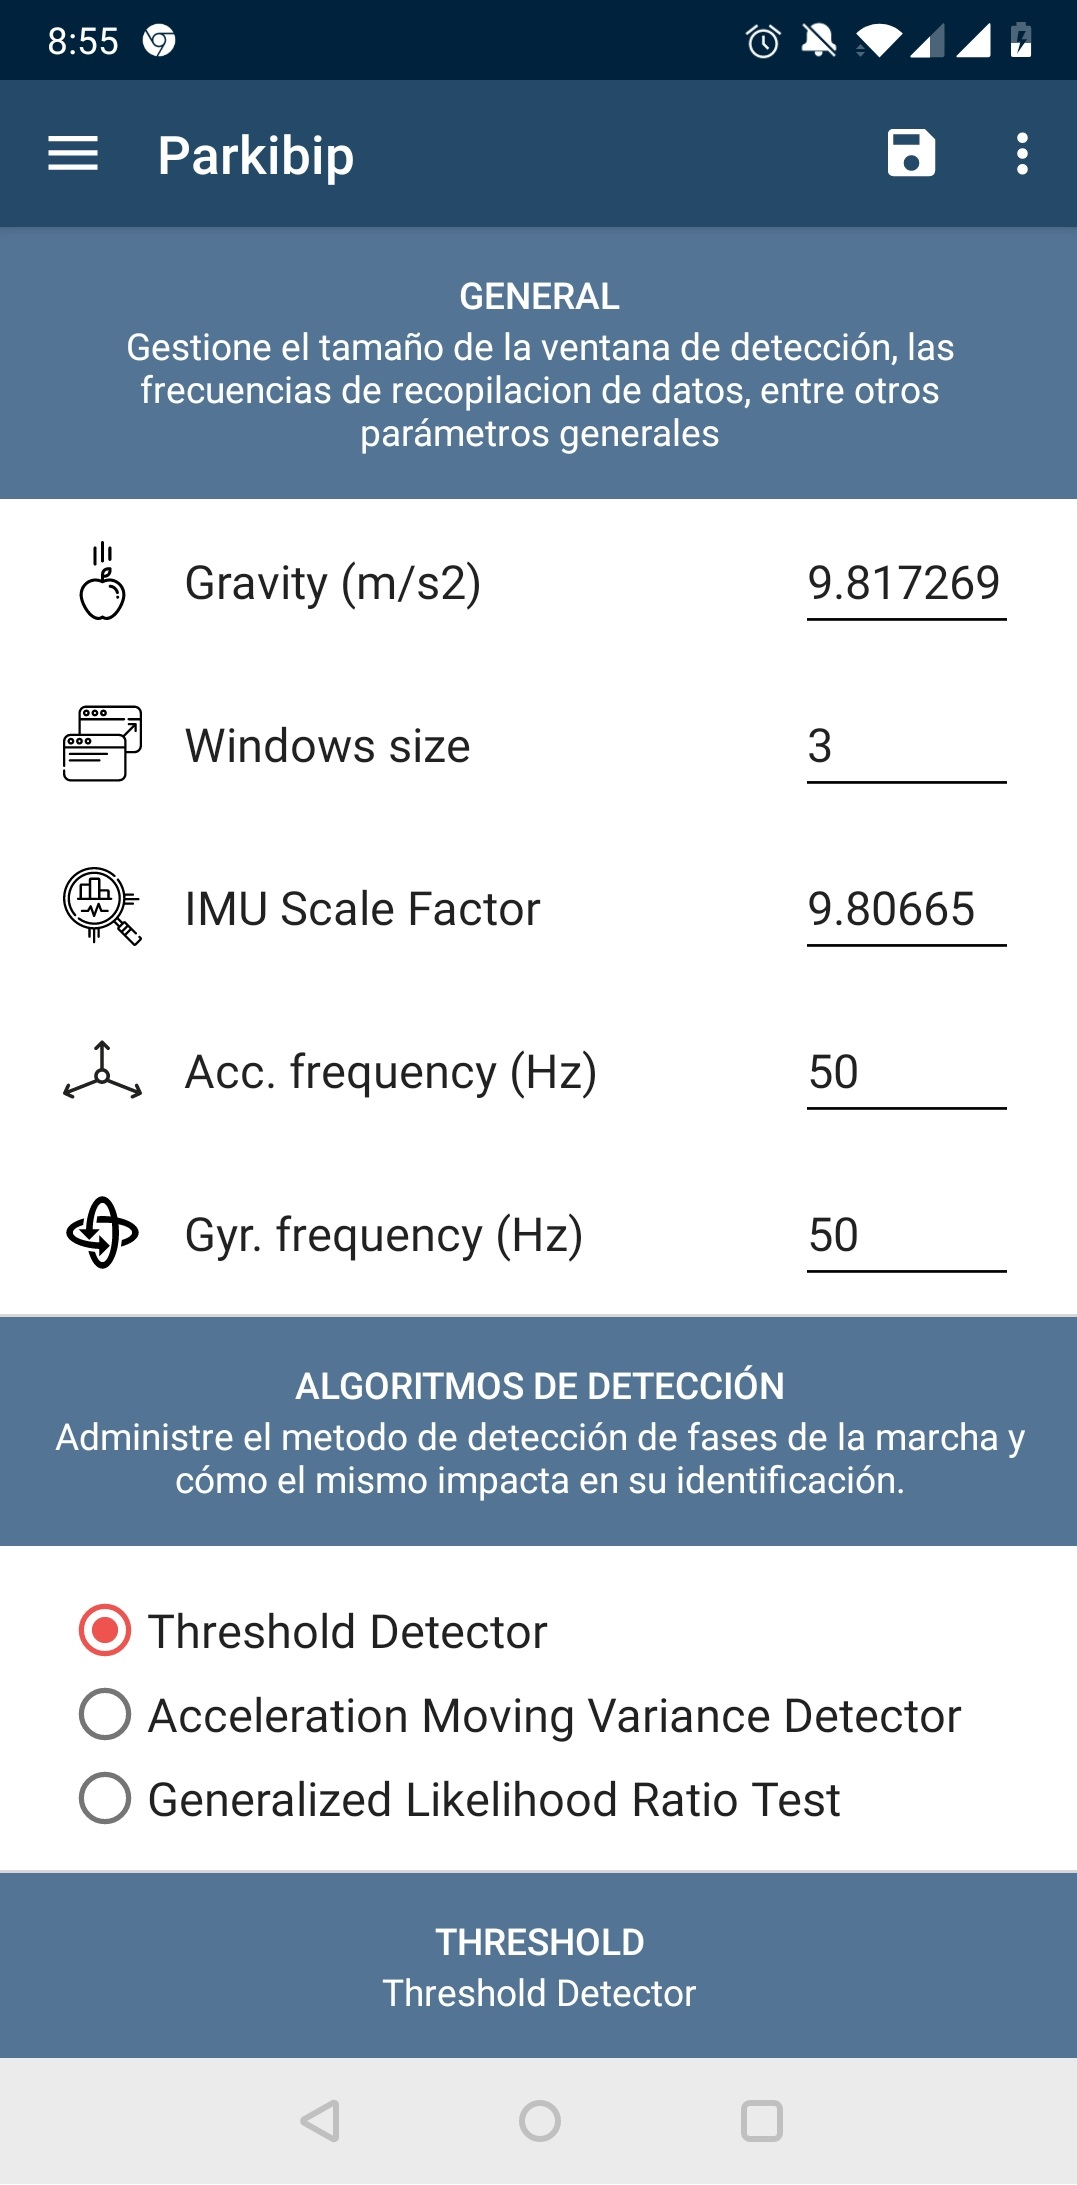
\includegraphics[height=8cm]{TESIS/imagenes/chap05/activity-configuration.JPG}
         \caption{Configuración de parámetros y selección del algoritmo de detección. PARKIBIP habilita al usuario a modificar parámetros generales y específicos de los métodos.}
     \end{subfigure}
     ~
     \begin{subfigure}[t]{0.4\textwidth}
         \centering
         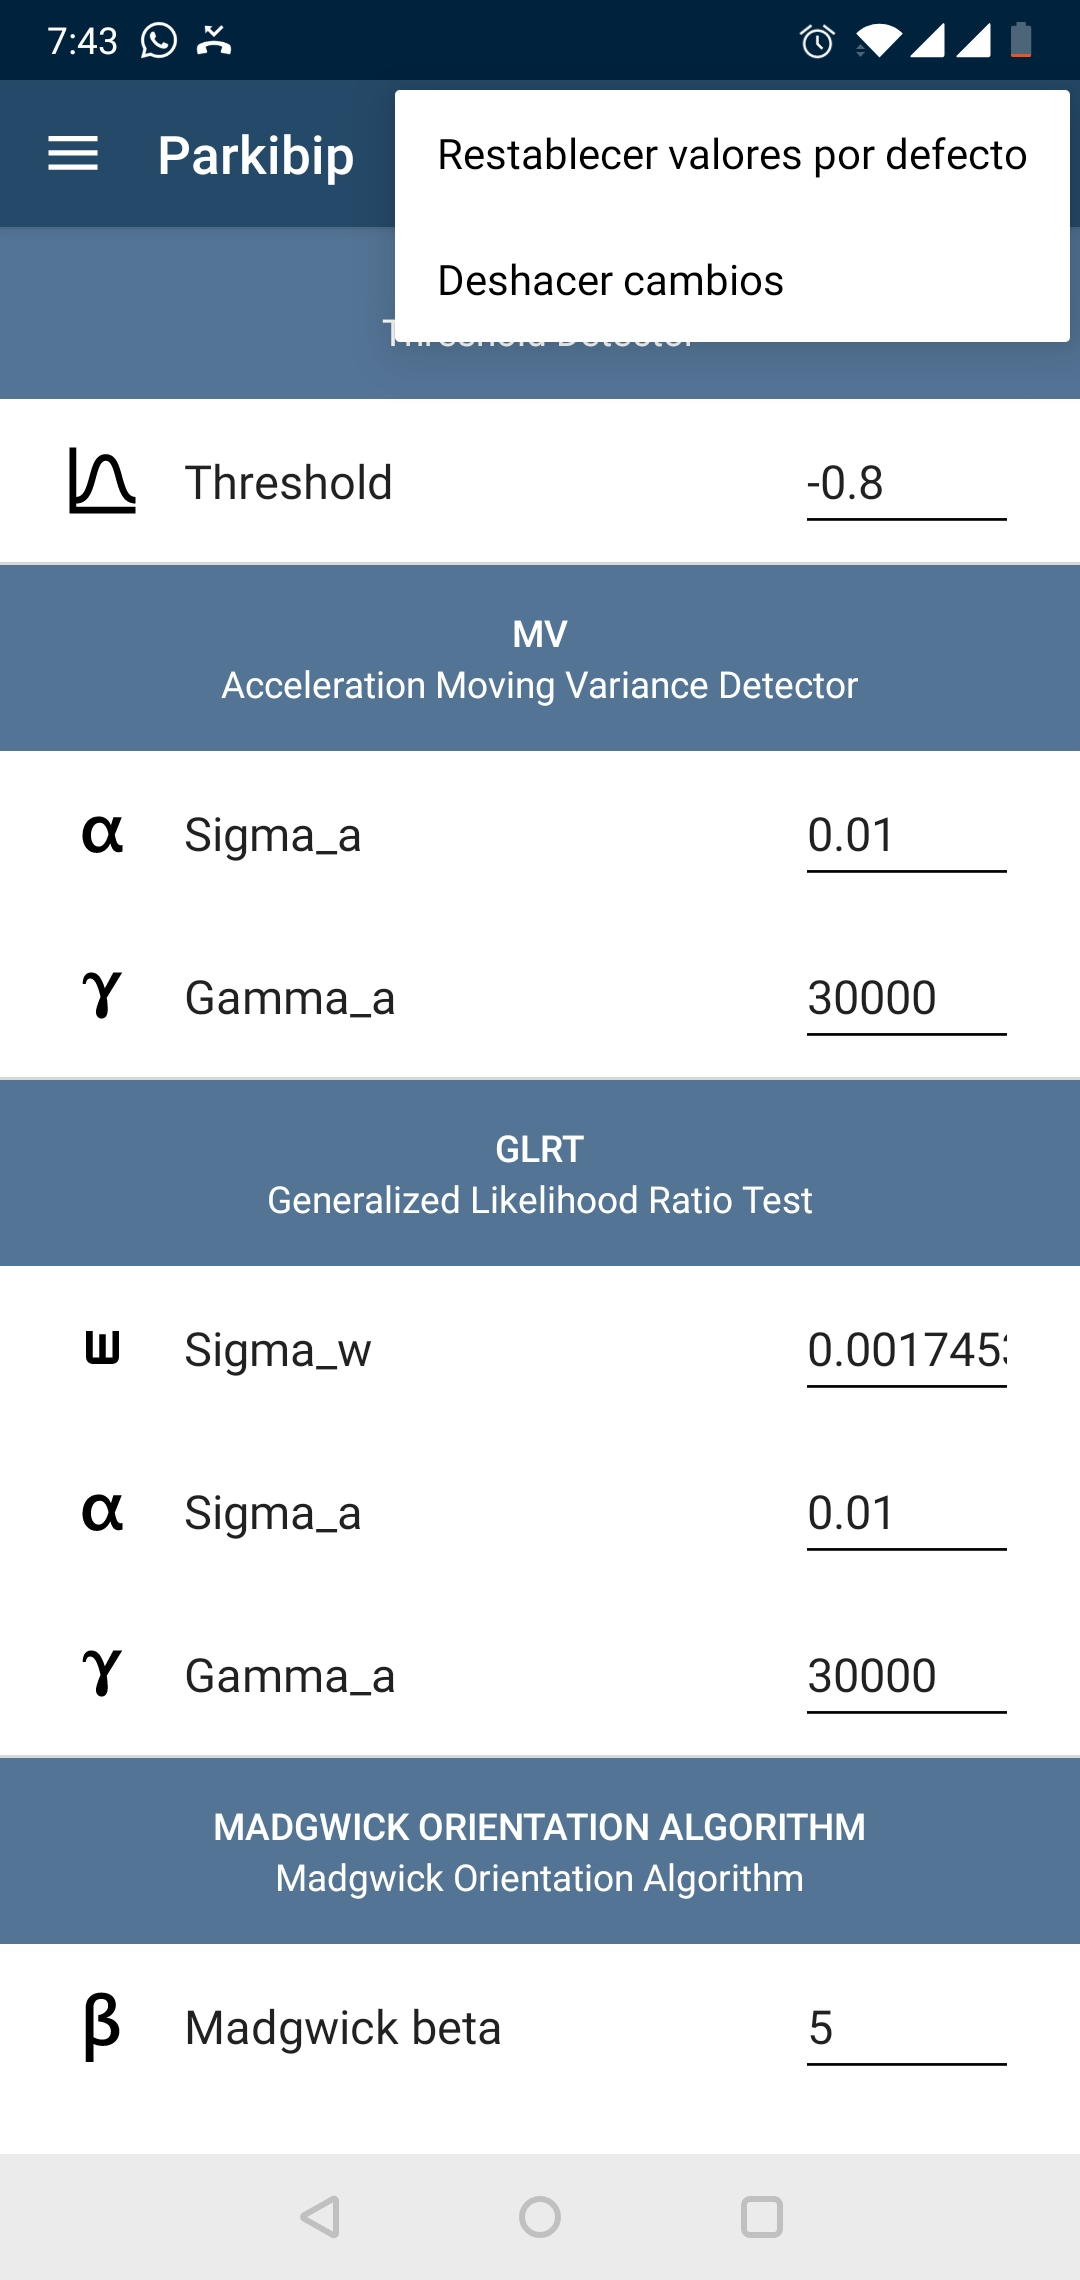
\includegraphics[height=8cm]{TESIS/imagenes/chap05/activity-configuration2.JPG}
         \caption{Restauración de valores. PARKIBIP permite restablecer a valores de fábrica, así como descartar cambios efectuados.}
     \end{subfigure}
     \caption{Configuración de parámetros generales y particulares a los detectores. Además, selección del algoritmo de detección.}
     \label{fig:activity-configuration}
 \end{figure}

\newpage

\section{Módulo de Biofeedback}

El módulo de \textit{Biofeedback} cumple una función esencial para PARKIBIP. Con una visión global, es el encargado de capturar y procesar los resultados de los distintos \textit{DataAnalyzer} -analizador creado para cada IMU-, los cuales procesan los datos, emiten eventos a dicho módulo -indicando la ocurrencia de un Heel Strike o un Toe Off- y además, notifican parámetros espacio-temporales como la posición, la velocidad y la orientación instantánea relativos a cada pie.  Así, el módulo de Biofeedback transforma la información recibida según reglas pre-definidas dentro del mismo, para estimular al usuario,  y luego calcula los datos de la sesión en tiempo real para ser mostrados en la pantalla. 

La figura Fig. \ref{FIG:biofeedback-module-class-diagram} presenta un diagrama del subsistema en el cual se encuentra el módulo de Biofeedback -representado con la clase \textit{BiofeedbackModule}-, donde se puede visualizar cuáles son las clases con las que el mismo interactúa.

\begin{figure}[H]
    \hspace*{-3.5cm}%
    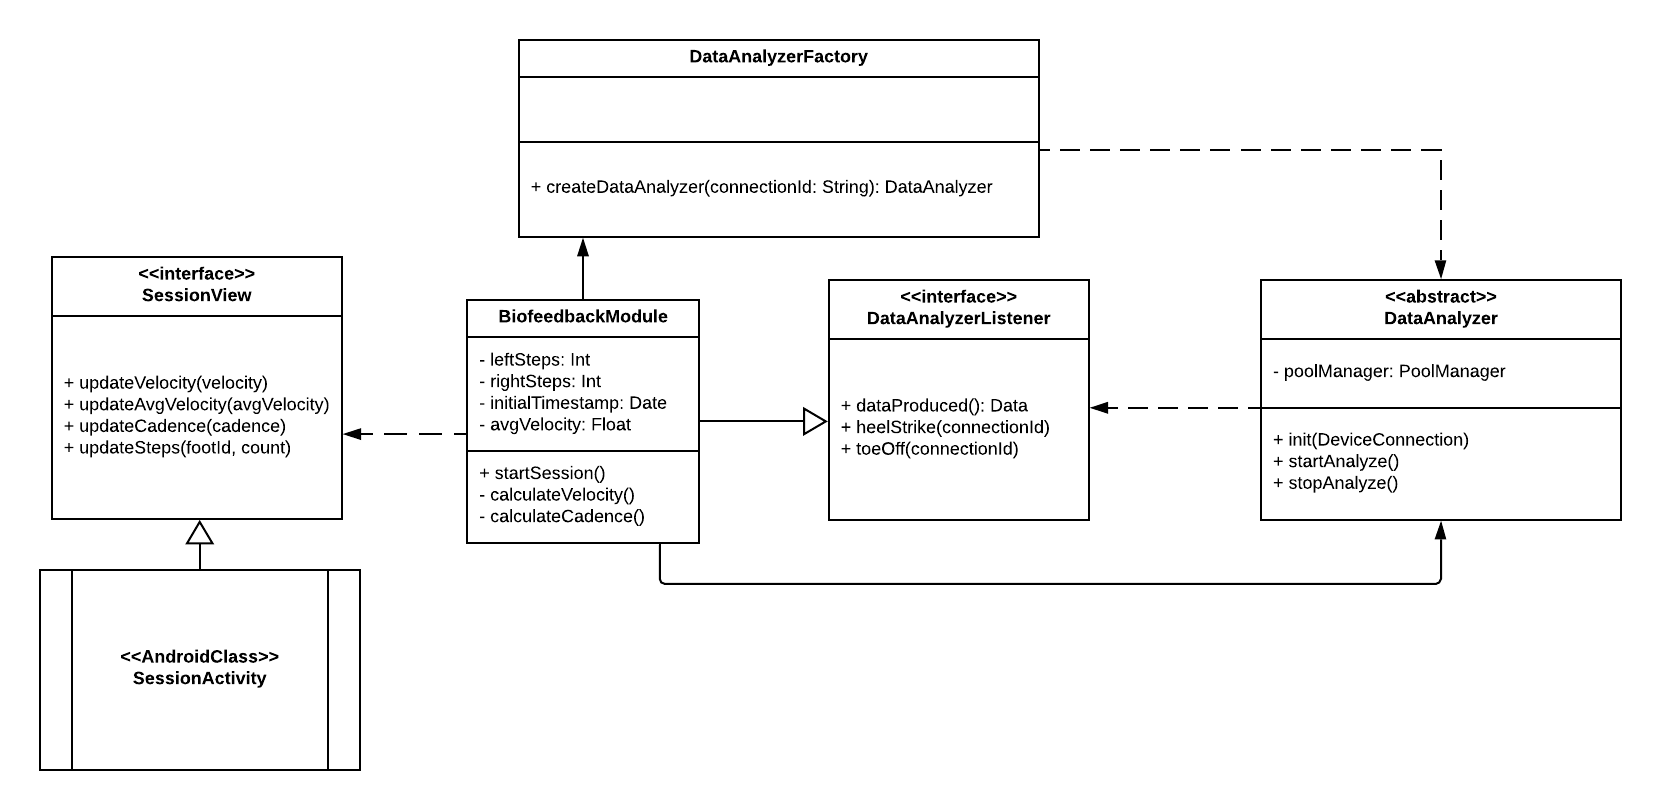
\includegraphics[clip,width=1.4 \columnwidth]{TESIS/imagenes/chap05/biofeedback-module-design.png}   
    \caption{Diagrama de clases del módulo de la aplicación Android que establece las reglas para estimular y calcula los parámetros espacio-temporales de la sesión en tiempo real}
    \label{FIG:biofeedback-module-class-diagram}
\end{figure}

Cuando es iniciada una sesión de fisioterapia con PARKIBIP, \textit{BiofeedbackModule} es quien solicita al \textit{DataAnalyzerFactory} la creación de los \textit{DataAnalyzer}, se suscribe a los eventos como su \textit{DataAnalyzerListener} manteniendo las referencias adecuadas. Para procesar los datos que produce cada \textit{DataAnalyzer}, implementa la interfaz \textit{DataAnalyzerListener}. Esta interfaz encapsula todos los métodos que utiliza el \textit{DataAnalyzer} para notificar a las clases interesadas los datos que obtiene como resultado del procesamiento. Así, los \textit{DataAnalyzer} notifican a su \textit{DataAnalyzerListener} cada vez que se produce un evento del tipo Heel Strike o Toe Off, como también las actualizaciones del vector de estado del algoritmo filtro de Kalman, el cual contiene posición, velocidad y orientación. 

\textit{BiofeedbackModule} emplea los entradas mencionadas para calcular los siguientes datos en tiempo real:

\begin{itemize}
    \item Velocidad instantánea para cada pie 
    \item Velocidad promedio de la marcha 
    \item Cantidad de pasos
    \item Cadencia (i.e pasos por minutos) 
    \item Duración media del paso 
    \item Aceleración instantánea para cada pie 
    \item Aceleración promedio de la marcha 
\end{itemize}

Este módulo, tiene además la capacidad de reaccionar a ciertas reglas pre-definidas y configurables conforme a estimular adecuadamente al paciente. Los niveles de estímulos para el paciente PARKIBIP son: 

\begin{itemize}
    \item Vibración en el dispositivo IMU utilizando el motor de vibración embebido en el dispositivo MetaMotionR.
    \item Sonido ``Beep'' emitido por la aplicación móvil, el cual es tan importante como para tener su referencia en el nombre del proyecto.
\end{itemize}

La figura Fig. \ref{fig:activity-active-session} ilustra una sesión PARKIBIP en curso. Tal como se puede apreciar, el sistema reacciona en tiempo real a la marcha del paciente en rehabilitación, mediante el envío de estímulos externos -vibración y/o sonido- y el cómputo de parámetros espacio-temporales. Así, medición a medición, la interfaz de usuario comienza a transitar por distintos valores fruto del procesamiento de PARKIBIP.  

\begin{figure}[H]
 \centering
 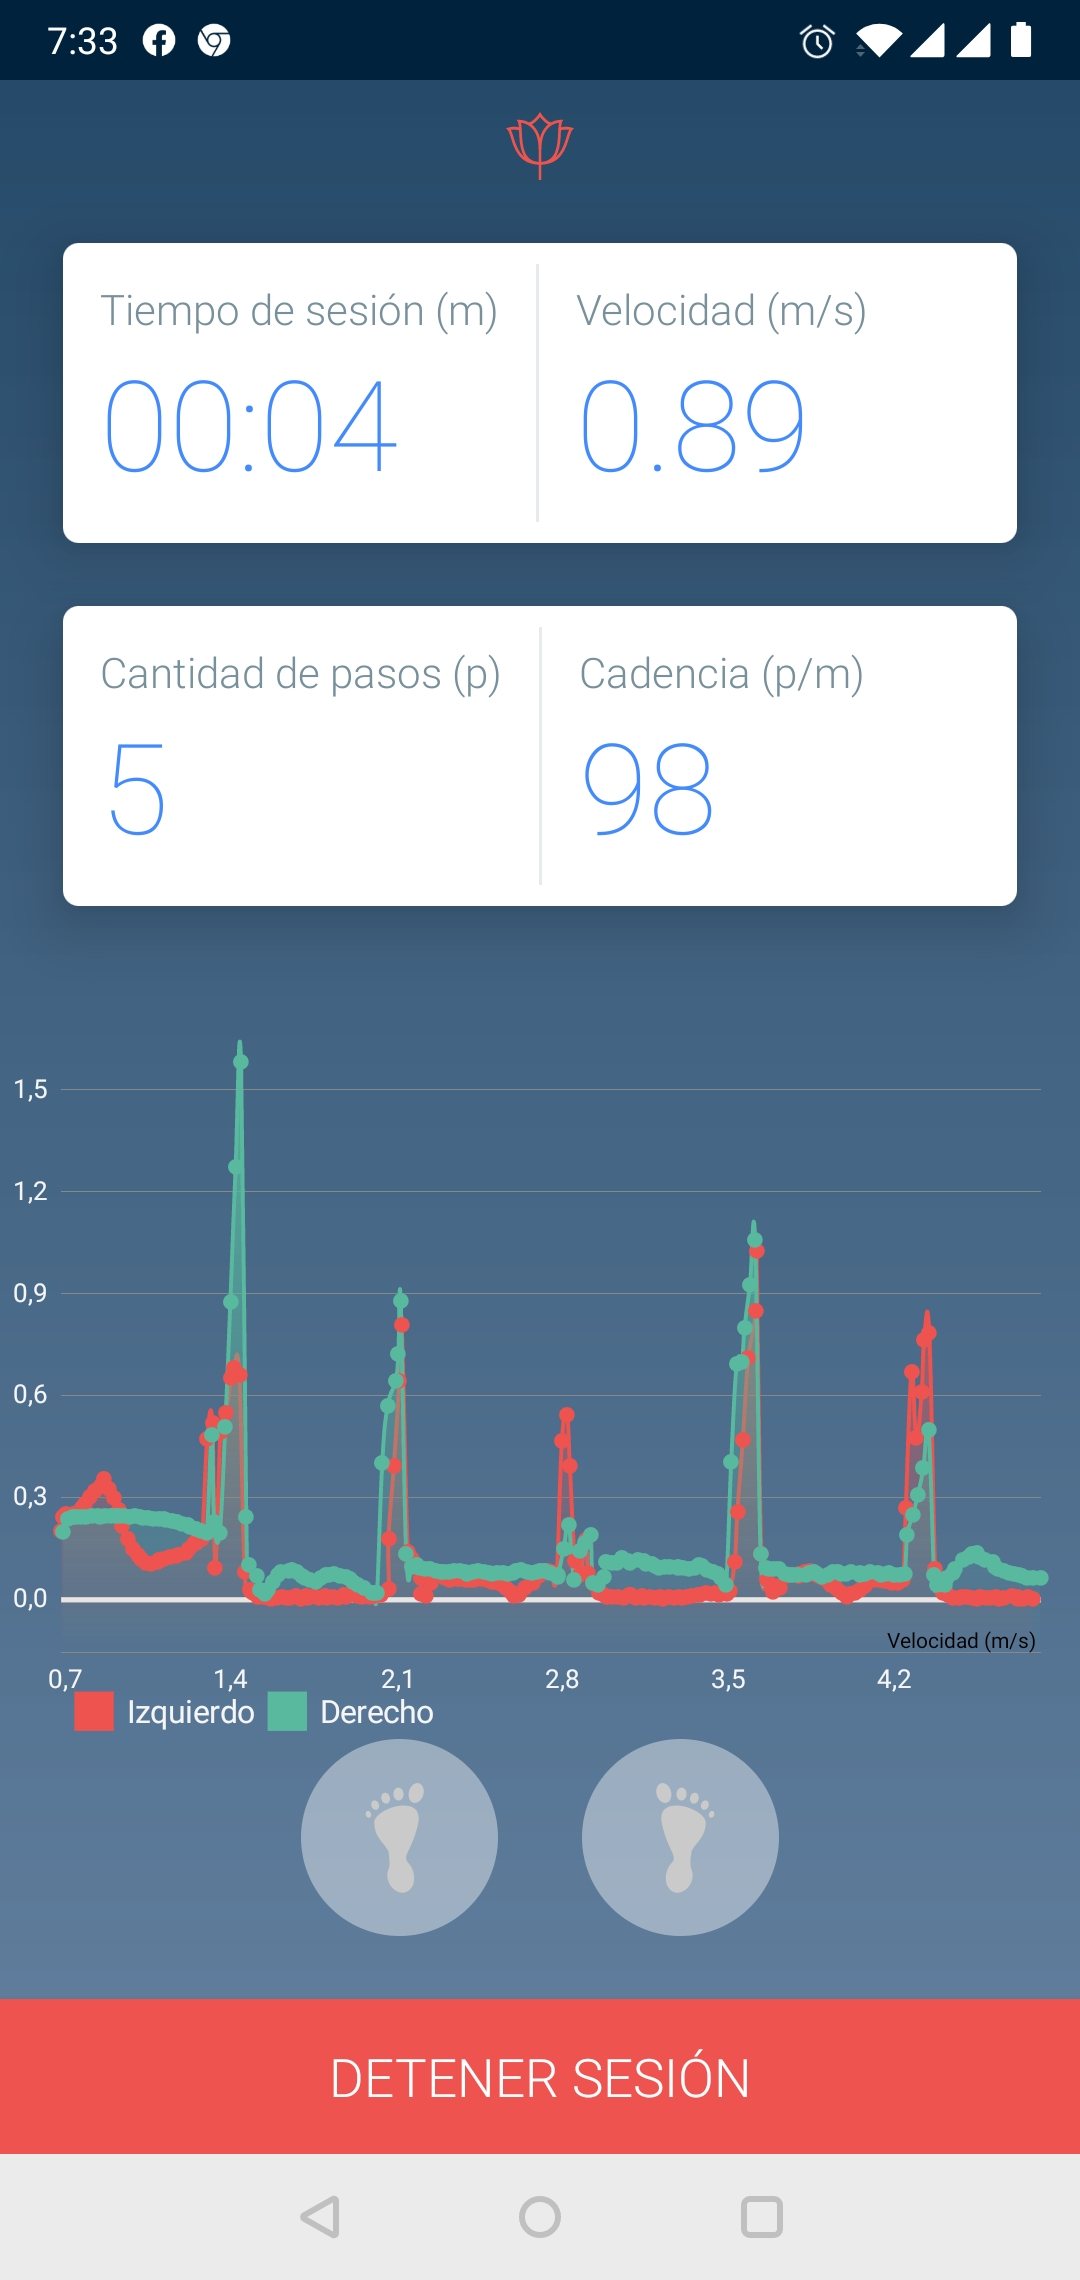
\includegraphics[height=9cm]{TESIS/imagenes/chap05/activity-active-session.JPG}
 \caption{Pantalla de una Sesión Activa PARKIBIP. El sistema reacciona en tiempo real a la marcha del paciente en rehabilitación. Dispara estímulos externos -vibración y/o sonido- y computa los parámetros espacio-temporales.}
 \label{fig:activity-active-session}
\end{figure}

Si bien las posibilidades son infinitas (i.e. debido a múltiples combinaciones de parámetros espacio-temporales), a continuación se detallan las principales reglas implementadas en PARKIBIP para decidir en qué momentos se producen dichos estímulos:

\begin{itemize}
    \item \textbf{On Heel Strike}: Cada vez que se produce un Heel Strike. Esta es una regla básica pero sumamente importante, ya que el funcionamiento correcto de la misma indica que se identifican adecuadamente los pasos de la marcha.
    \item \textbf{On FoG}: Transcurrido un intervalo de tiempo pre-definido sin que ocurra un Heel Strike. Esta regla es útil para detectar un evento de FoG (Bloqueo de la marcha), y a través del estímulo buscar interrumpirlo. 
    \item \textbf{On Instant Velocity Threshold}: Al atravesar umbrales de velocidad instantánea. En este caso se le notifica al paciente a través de estímulos sobre la velocidad instantánea, que la misma es muy alta o muy baja y podría ocasionar, por ejemplo, una caída por mayor velocidad.  
    \item \textbf{On Average Velocity Threshold}: Al atravesar umbrales de velocidad promedio. En este caso se le notifica al paciente mediante estímulos que el ritmo es demasiado bajo o alto. 
    \item \textbf{On Dynamic Calculated Time}: Ocurre luego de cierto intervalo de tiempo calculado en forma dinámica a partir de una primera caminata de configuración. Por ejemplo, el paciente realiza una marcha inicial de 6 pasos, y en base a los datos recopilados se computa el tiempo promedio entre los mismos. Luego, el estímulo vibratorio y/o sonoro se realiza en un periodo constante definido por este tiempo calculado -simulando una terapia rítmica de rehabilitación-. Desde el punto de vista terapéutico, podría resultar que la caminata del paciente sea demasiado lenta o demasiado rápida, por lo que el tiempo promedio calculado a partir de su caminata inicial no sería un buen indicador para efectuar el estímulo. Sin embargo, podría ser de utilidad para evaluar al paciente en deambulación respecto al ritmo de marcha y su uniformidad. 
\end{itemize}

Muchas de las grandes oportunidades de mejora que presenta el sistema, para ser implementadas a futuro, resultan de mejorar este módulo, ya sea implementando nuevas reglas o incrementando la inteligencia del mismo para decidir en qué momentos estimular. Además, se podrían crear nuevos tipos de estímulos, como por ejemplo el habla en lenguaje natural.

\section{Caso de uso: Flujo automatizado de Sesión Activa PARKIBIP}
\label{section:session-flow}

En línea con los subprocesos desarrollados y mencionados con anterioridad, se propone el caso de uso de Sesión Activa, fundamental para lograr comprender el funcionamiento de fondo de PARKIBIP. De esta manera, se elaboró el diagrama Fig. \ref{FIG:use-case-session}, que modela el flujo de tareas e información mediante la notación estándar BPMN 2.0.

Como se puede apreciar en la figura, el modelo integra los distintos componentes (e.g. \textit{DeviceConnection}, \textit{DataAnalyzer}, \textit{Services}, \textit{Threads}, \textit{Queues}, entre otros) y algoritmos numéricos desarrollados (e.g. filtro de Orientación, filtro de kalman, ZVD); luego los combina conforme a proponer una sinergia de trabajo que aumente el rendimiento del sistema, minimice el retardo de transmisión de eventos (por ende, los estímulos) y mantenga las responsabilidades bien delineadas (i.e. bajo acoplamiento y alta cohesión entre componentes). 

Para una mayor claridad y comprensión, el diagrama sintetiza el flujo a un único dispositivo inercial (en PARKIBIP, \textit{DeviceConnection}), esto significa que, existirán tantos componentes \textit{DataAnalyzers} con sus correspondientes \textit{KalmanFilterThreads} como dispositivos IMU o \textit{DeviceConnection} operando.

\newpage

\begin{figure}[H]
    \vspace{-3.0cm}
    \hspace*{-2.0cm}%
    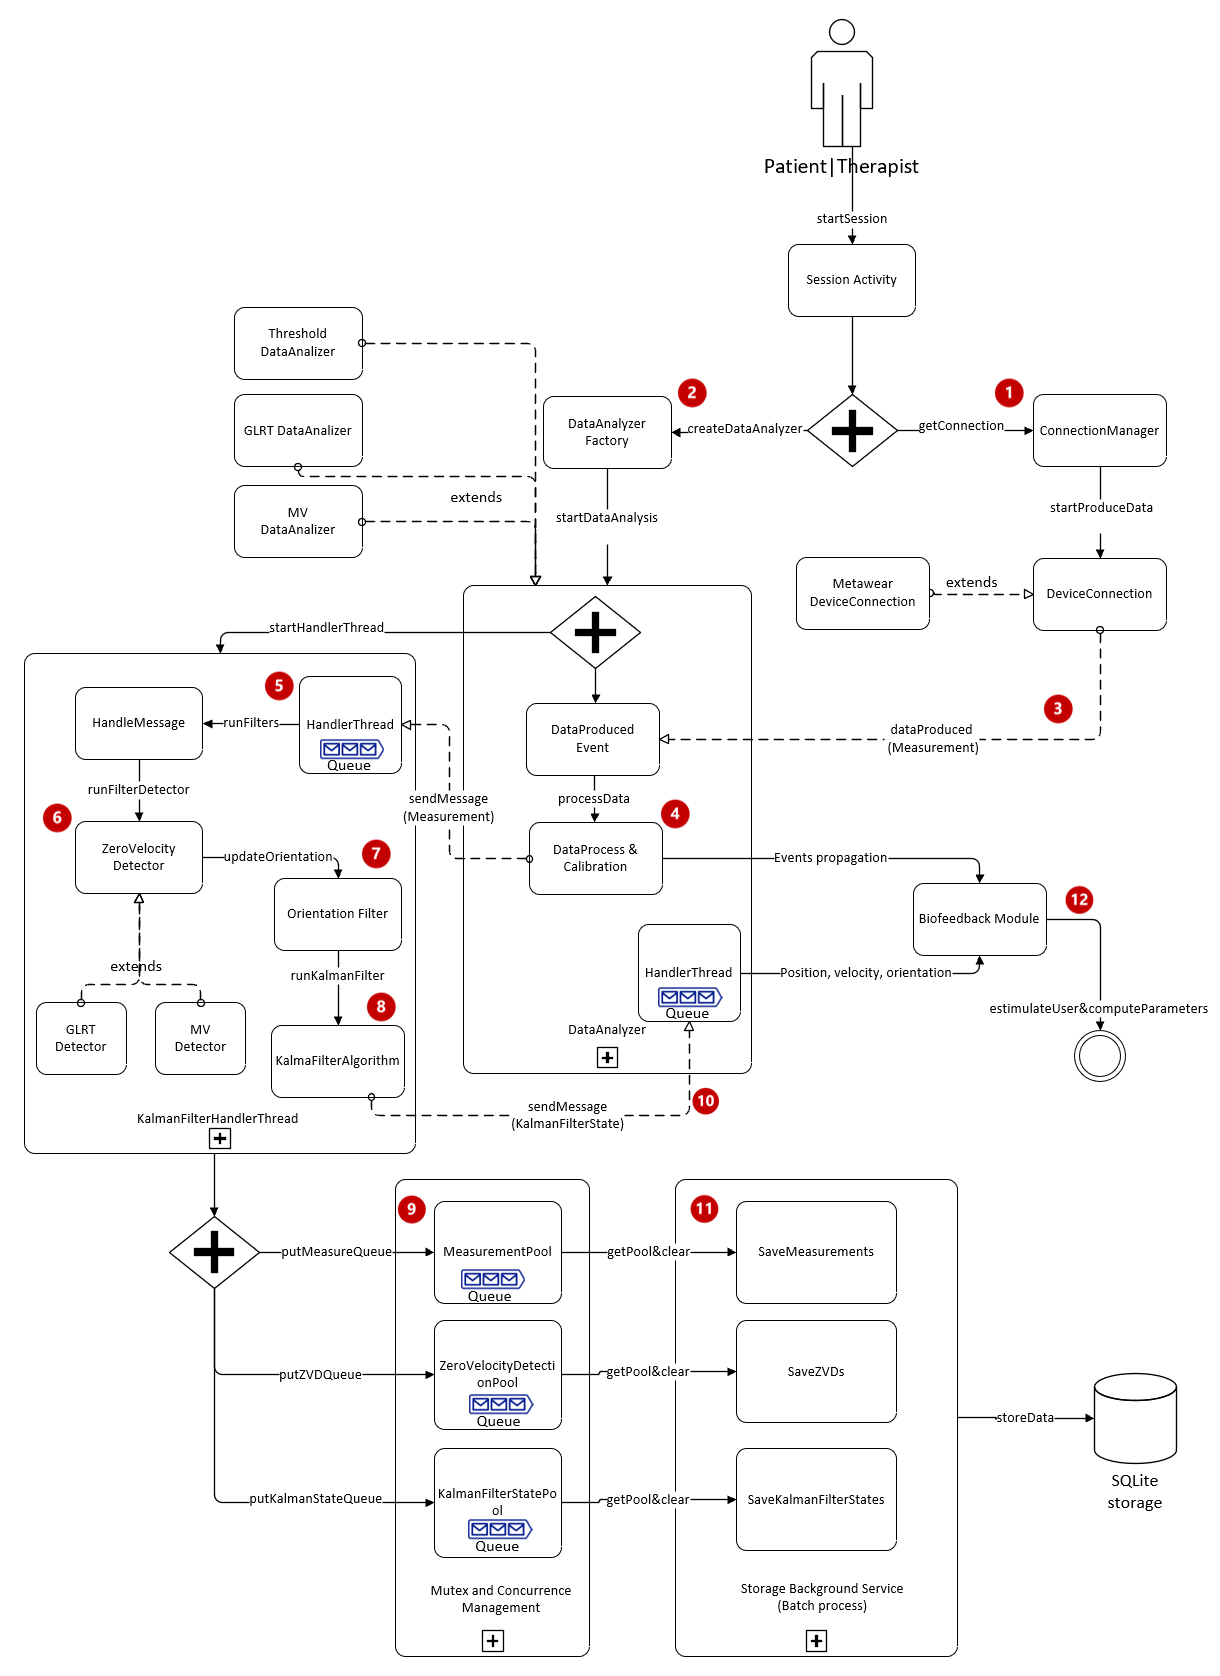
\includegraphics[clip,width=1.20 \columnwidth]{TESIS/imagenes/chap05/use-case-session.PNG}
    \caption{Flujo automatizado de Sesión Activa PARKIBIP. El modelo integra y combina los distintos componentes (e.g. \textit{DeviceConnection}, \textit{DataAnalyzer}, \textit{Services}, \textit{Threads}, \textit{Queues}, entre otros) y algoritmos numéricos que fueron desarrollados (e.g. filtro de Orientación, filtro de kalman, ZVD) con el fin de cumplir los objetivos del Proyecto. }
    \label{FIG:use-case-session}
\end{figure}

El Caso de Uso comienza cuando, un Terapeuta en una actividad de rehabilitación o un Paciente autónomo, inicia una Sesión previamente configurada en la aplicación PRKIBIP. En consecuencia, se disparan los eventos numerados en el diagrama Fig. \ref{FIG: ciclo}, y descriptos como notas al pie en lo que sigue:

\begin{enumerate}
    \item Mediante el manejador de conexiones -\textit{ConnectionManager}-, se obtiene la instancia lógica del dispositivo IMU particular a iniciar, un \textit{DeviceConnection} implementado por \textit{MetawearDevice}, cuya conexión fue previamente establecida. Luego de que se hayan establecido todas las configuraciones de los sensor y habilitado los productores de datos asíncronos, el sistema procede a iniciar la producción de datos de los distintos sensores. 
    \item De forma paralela, PARKIBIP crea un analizador de datos o \textit{DataAnalyzer} mediante la fábrica que encapsula dicha función -\textit{DataAnalyzerFactory}-. El tipo de \textit{DataAnalyzer} concreto a instanciar, dependerá de la selección vigente del mismo en el componente de configuraciones. Además, el sistema prepara e inicializa la recepción de eventos de datos de mediciones. En este punto, es importante resaltar que, el \textit{DataAnlyzer} será el responsable de orquestrar el procesamiento de la información a través de la delegación de tareas a ciertos módulos específicos.
    \item Cuando un sensor del IMU envía un evento de medición, éste es recibido mediante el componente \textit{DeviceConnection}; que analiza la secuencia de símbolos y la transforma a una estructura legible en la aplicación -modelo \textit{MeasurementModel}-. Luego, realiza un procesamiento previo del modelo de medición, ajustando las unidades al sistema internacional correspondiente y estandarizando la información.  Finalmente, dispara un evento de producción de datos a su \textit{DataAnalyzer} asociado.
    \item Recibido un evento de medición en el \textit{DataAnalyzer}, éste procede a ejecutar el flujo de procesamiento. En caso de que se requiera  calibrar la orientación del dispositivo IMU, el sistema realiza el el proceso de Calibración y descarta la medición. En otro caso, envía un evento de medición al manejador o \textit{Handler} del componente \textit{KalmanFilterHandlerThread}, así como también procesa la medición según el \textit{DataAnalyzer} concreto elegido. El resultado del procesamiento se propaga como evento al módulo de \textit{Biofeedback} de la aplicación.
    \item Primero, es crucial comprender el comportamiento de \textit{KalmanFilterHandlerThread}. Un Thread, representa un hilo de ejecución independiente al hilo principal de una aplicación; mientras que un \textit{HandlerThread} -en Android-, es una extensión del Thread que integra el concepto de \textit{Looper} y de \textit{Handler}. Un \textit{Looper} dentro de un Thread, tiene la capacidad de administrar adecuadamente los múltiples mensajes recibidos mediante su manejador -\textit{Handler}- y su estructura de almacenamiento del tipo Cola FIFO (del inglés, Queue). Entonces, el evento de medición recepcionado por el \textit{Handler} de \textit{KalmanFilterHandlerThread}, es inicialmente puesto en la Cola del \textit{Looper}, y luego atendido por el método \textit{HandleMessage}.
    \item La función \textit{HandleMessage}, responsable del procesamiento del filtro de Kalman, comienza ejecutando el detector de cero velocidad -\textit{ZeroVelociyDetector}-, dato requerido como parámetro por Kalman. El ZVD  concreto a emplear (e.g. GLRT, MV), se obtiene de la configuración actual del sistema.
    \item Luego, es vital la actualización de la orientación con cada medición entrante, no solo por
    ser pre-condición del algoritmo de Kalman, sino también para minimizar errores en la predicción de los parámetros espacio-temporales futuros. Por consiguiente, se corre el filtro de Orientación propuesto por S.Madwick en \cite{Madgwick}.
    \item Junto a la medición recopilada y los parámetros orientación y momento de velocidad cero -\textit{z\_value}-, el sistema ejecuta el filtro de Kalman. Este método es iterativo a medida que su función de actualización es invocada, y arroja como resultado un vector de estados con las estimaciones: posición, velocidad y orientación. Además, con el parámetro \textit{z\_value}, el algoritmo compensa/corrige las estimaciones según si el IMU se encuentra estacionario.
    Finalmente, el \textit{HandlerThread} de \textit{KalmanFilter} dispara un evento de mensajes hacia el \textit{Handler} del \textit{DataAnalyzer}, encapsulando el vector de estados resultante del procesamiento. A su vez, en paralelo, envía el modelo de medición y los resultados de cada algoritmo numérico -\textit{z\_value}, vector de kalman- a sus respectivos conjuntos de datos (en inglés, Data Pool).
    \item Cada unidad de \textit{Data Pool}, gestiona el acceso concurrente mediante la mutua exclusión de sus estructuras y recursos (e.g. Colas de mensajes). Los datos son puestos en el pool desde el hilo de ejecución Kalman, y recuperados en batch por un servicio de sistema de fondo.
    \item Análogo al punto 5, el mensaje con el vector de estados es recibido por el \textit{Handler} del \textit{DataAnalyzer} y puesto en la Cola del \textit{Looper}. En esta ocasión, el \textit{DataAnalyzer} actúa como pasamanos de información, propagando el estado hacia el modulo de \textit{Biofeedback}.
    \item Un servicio en Android, es un componente de una aplicación que puede realizar operaciones de larga ejecución en segundo plano. En PARKIBIP, cumple la responsabilidad del almacenamiento de datos en la base de datos SQL de la aplicación móvil. Con una frecuencia configurable y repetitiva, el servicio obtiene los datos a almacenar desde los Pooles de datos -en batch-, los vacía, y luego almacena los elementos en la base de datos.
    \item Concluyendo el proceso, el módulo de \textit{Biofeedback}, responsable de disparar los eventos de estimulación al Paciente, ejecuta las reglas clínicas apropiadas.
\end{enumerate}

\section{Administración de Identidades}

El sistema PARKIBIP fue diseñado específicamente para administrar dos niveles de usuarios, el Terapeuta y el Paciente en rehabilitación. En consecuencia, resulta imprescindible contar con un módulo particular, responsable de gestionar todas las funcionalidades requeridas para llevar adelante la gestión de identidades, proveer seguridad, y especialmente preservar la privacidad del Paciente. 

Así, en el presente apartado, se cubren detalles de la solución en cuanto a la administración de identidades, los protocolos que se deben usar y el flujo de autenticación requerido.

PARKIBIP decidió utilizar Auth0 \cite{Auth0}, como su proveedor de identidad como servicio (Identity as a Service, IDaaS, por sus siglas en inglés). Un IDaaS es un servicio basado en la nube para la gestión de identidades y accesos, a menudo también incluyen el inicio de sesión único (en inglés Single Sign-on, SSO), identidad federada, administración de contraseñas, entre otros. El razonamiento detrás de esta decisión fue la de integrar un servicio de terceras partes dedicado en la materia, y no implementar/mantener todos los aspectos complejos relativos a la seguridad, requeridos en ambientes productivos para datos sensibles. También, fue considerado y preparado en el diseño de la solución, la posibilidad de reemplazar fácilmente el módulo IDaaS por un nuevo micro-servicio (e.g. Agesic). Auth0 es una solución flexible y sencilla para agregar servicios de autenticación y autorización a las aplicaciones. De esta manera, el equipo y la organización pueden evitar el costo, el tiempo y el riesgo que conlleva la creación de su propia solución para autenticar, autorizar, discriminar y obtener información de los usuarios.

En definitiva, la aplicación Android PARKIBIP fue integrada a el proveedor de IDaaS Auth0 mediante el SDK del segundo, desarrollada en el lenguaje JAVA para Android y diseñada según la figura Fig. \ref{fig:activity-login}. 

\begin{figure}[H]
 \centering
 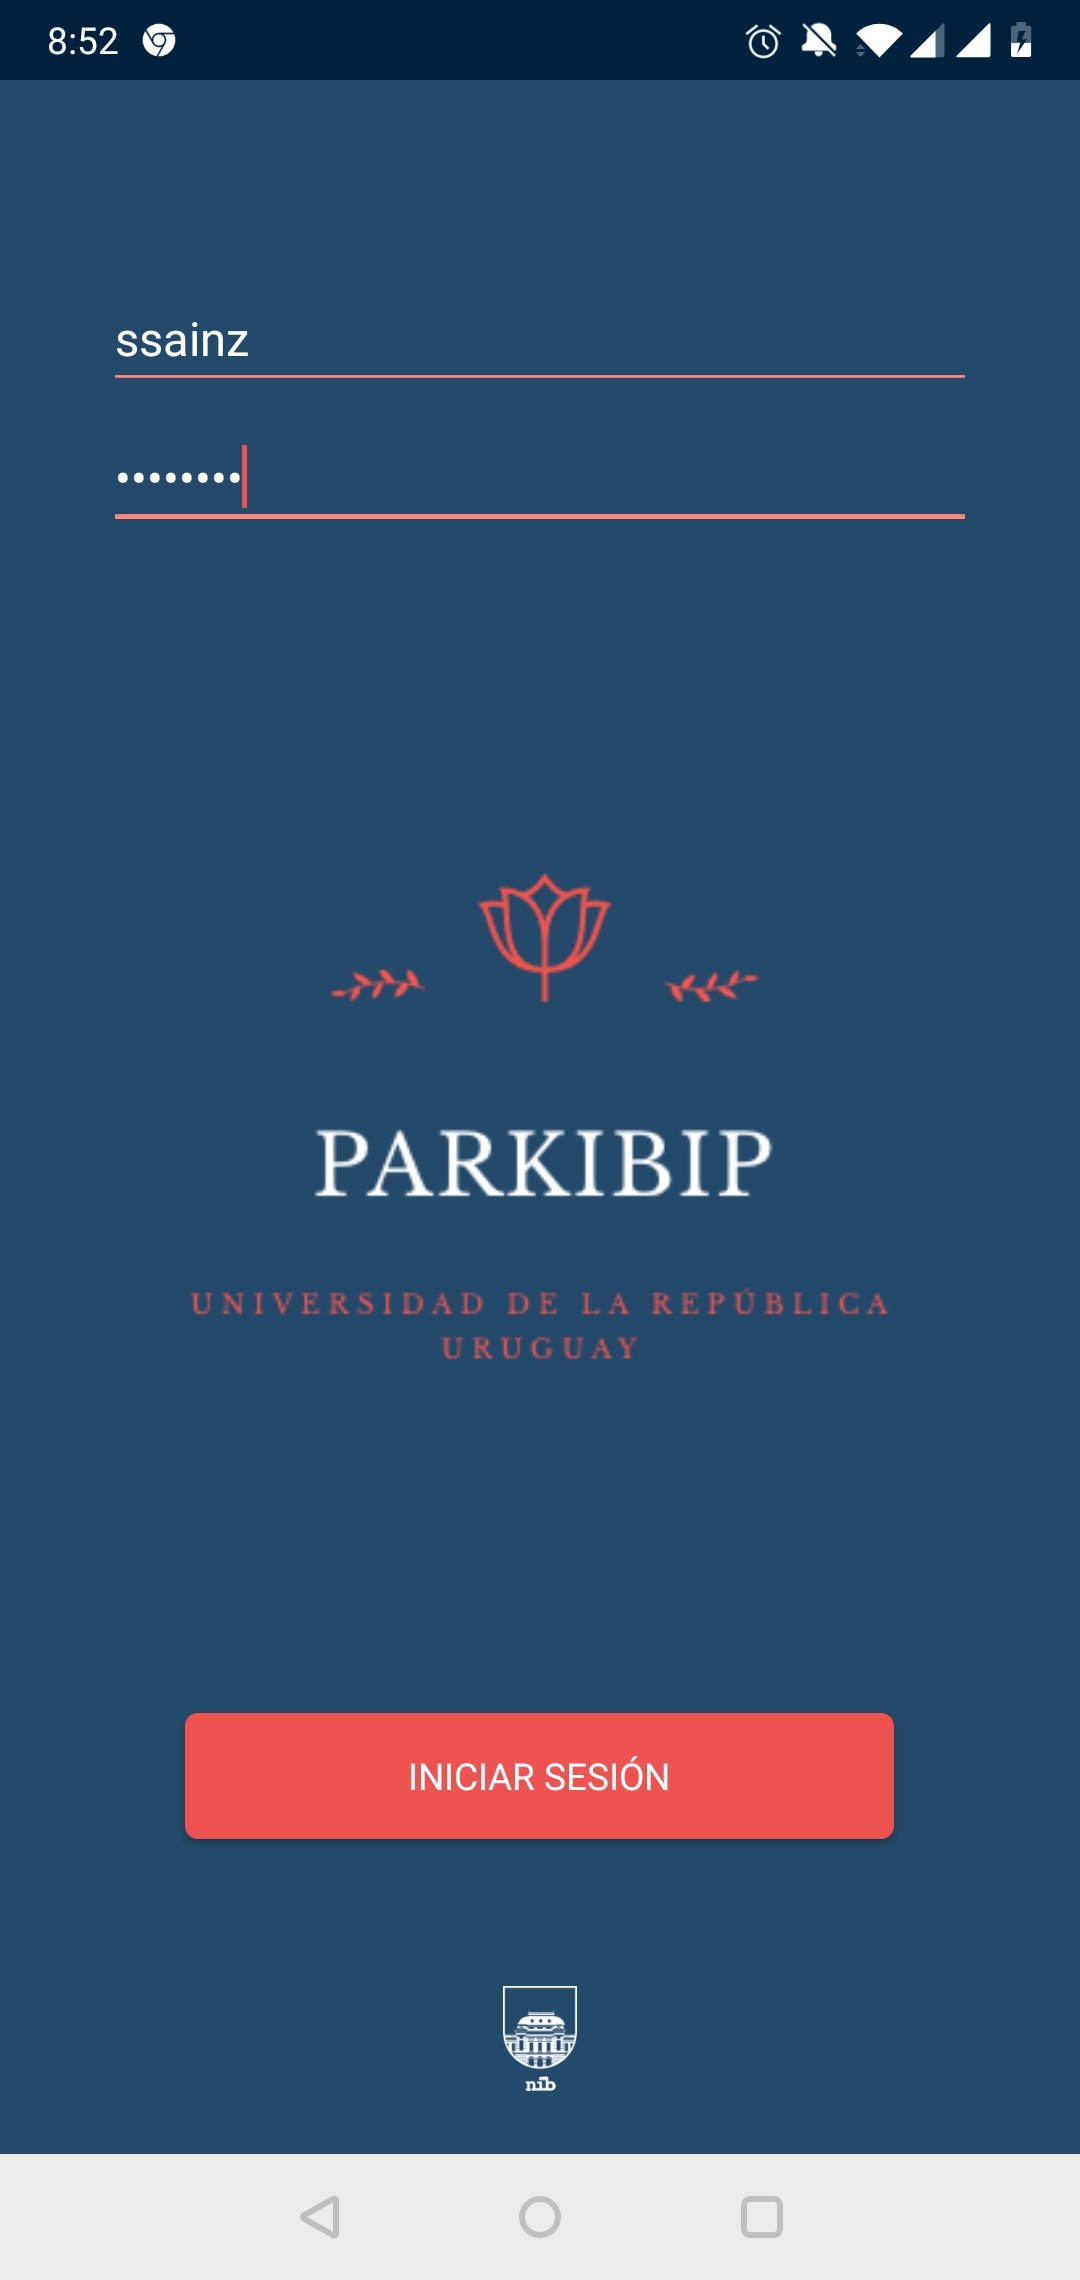
\includegraphics[height=8cm]{TESIS/imagenes/chap05/activity-login.JPG}
 \caption{Proceso de autenticación y autorización del Usuario. Se requieren los campos nombre de usuario y contraseña.}
 \label{fig:activity-login}
\end{figure}

En términos generales, para efectuar esta tarea se realizaron las configuraciones:

\begin{enumerate}
    \item Primero, fue creado un Auth0 tenant. Aquí es donde se configura el uso de Auth0, y donde los activos y recursos, como aplicaciones, conexiones y perfiles de usuario, se definen, administran y almacenan.
    \item Luego, se registró una aplicación nativa o móvil (en inglés, Native/Mobile App) que indica el tipo de aplicación que empleará los servicios en el \textit{Dashboard} de Auth0. Registrado el nuevo cliente, se obtuvo un ID de cliente único, necesario para efectuar llamados a las distintas funciones de la API de Auth0. Otro dato crucial, es el secreto del cliente (del inglés, Client Secret), análogo a una contraseña de aplicación que debe mantenerse confidencial en todo momento.
    \item Además, fue configurada la conexión que indica cómo los usuarios de PARKIBIP iniciarán sesión. Para ello, se uso la base de datos en la nube de Auth0.
    \item Finalmente, se implementaron las llamadas Reglas (Rules, en inglés). Estas, son funciones escritas en los lenguajes de programación JavaScript o C\#, ejecutadas en el mismo servidor de Auth0 justo después de una autenticación exitosa y antes de que el control regrese a la aplicación que realizo la invocación. Por ejemplo, fueron usadas para adjuntar en el Token información codificada del usuario.
\end{enumerate}

Otro aspecto importante, fue la manipulación del protocolo estándar abierto (RFC 7519) \textit{JSON Web Token} (JWT). El token JWT define una forma compacta y autónoma de transmitir información de forma segura entre las partes involucradas en el intercambio, como un objeto JSON. Dicha información puede ser verificada y confiada, ya que la misma está firmada digitalmente. Los JWT se pueden firmar usando el \textit{Client Secret} con el algoritmo de cifrado HMAC, o mediante el par de claves pública/privada empleando los algoritmos criptográficos RSA o ECDSA. En PARKIBIP se empleó el cifrado RS256 como algoritmo de firma digital para los \textit{JsonWebTokens}, en donde se firmará con la clave de firma privada y se puede verificar utilizando la clave de firma pública. Emplear JWT presenta variadas ventajas en comparación con los tokens web simples, y es usado con los siguientes objetivos:

\begin{itemize}
    \item Autenticación: cuando un usuario inicia sesión con éxito mediante sus credenciales, se devuelve un token de identificación -\textit{id\_token}- del tipo JWT.
    \item Autorización: una vez que un usuario ha iniciado sesión correctamente, PARKIBIP solicita acceso a rutas, servicios o recursos (por ejemplo, API) en nombre de ese usuario. Para hacerlo, en cada solicitud, debe pasar un Token de acceso -\textit{access\_token}-.
    \item Intercambio de información: Los JWT son una buena forma de transmitir información de forma segura entre las partes -firma digital-. 
\end{itemize} 

La figura Fig. \ref{FIG:payload-token} presenta un ejemplo de carga útil (del inglés Payload) encapsulada en el \textit{id\_token} durante el intercambio de información. Se aprecian metadatos del usuario, información descriptiva y transaccional del mismo. Valga como ejemplo el nombre, email, rol o tipo de usuario en el sistema, fecha de alta, entre otros. Por ende, el módulo de identidad de PARKIBIP, se encarga de interpretar el JSON conforme a acceder a los atributos de interés.

\begin{figure}[h!]
\centering
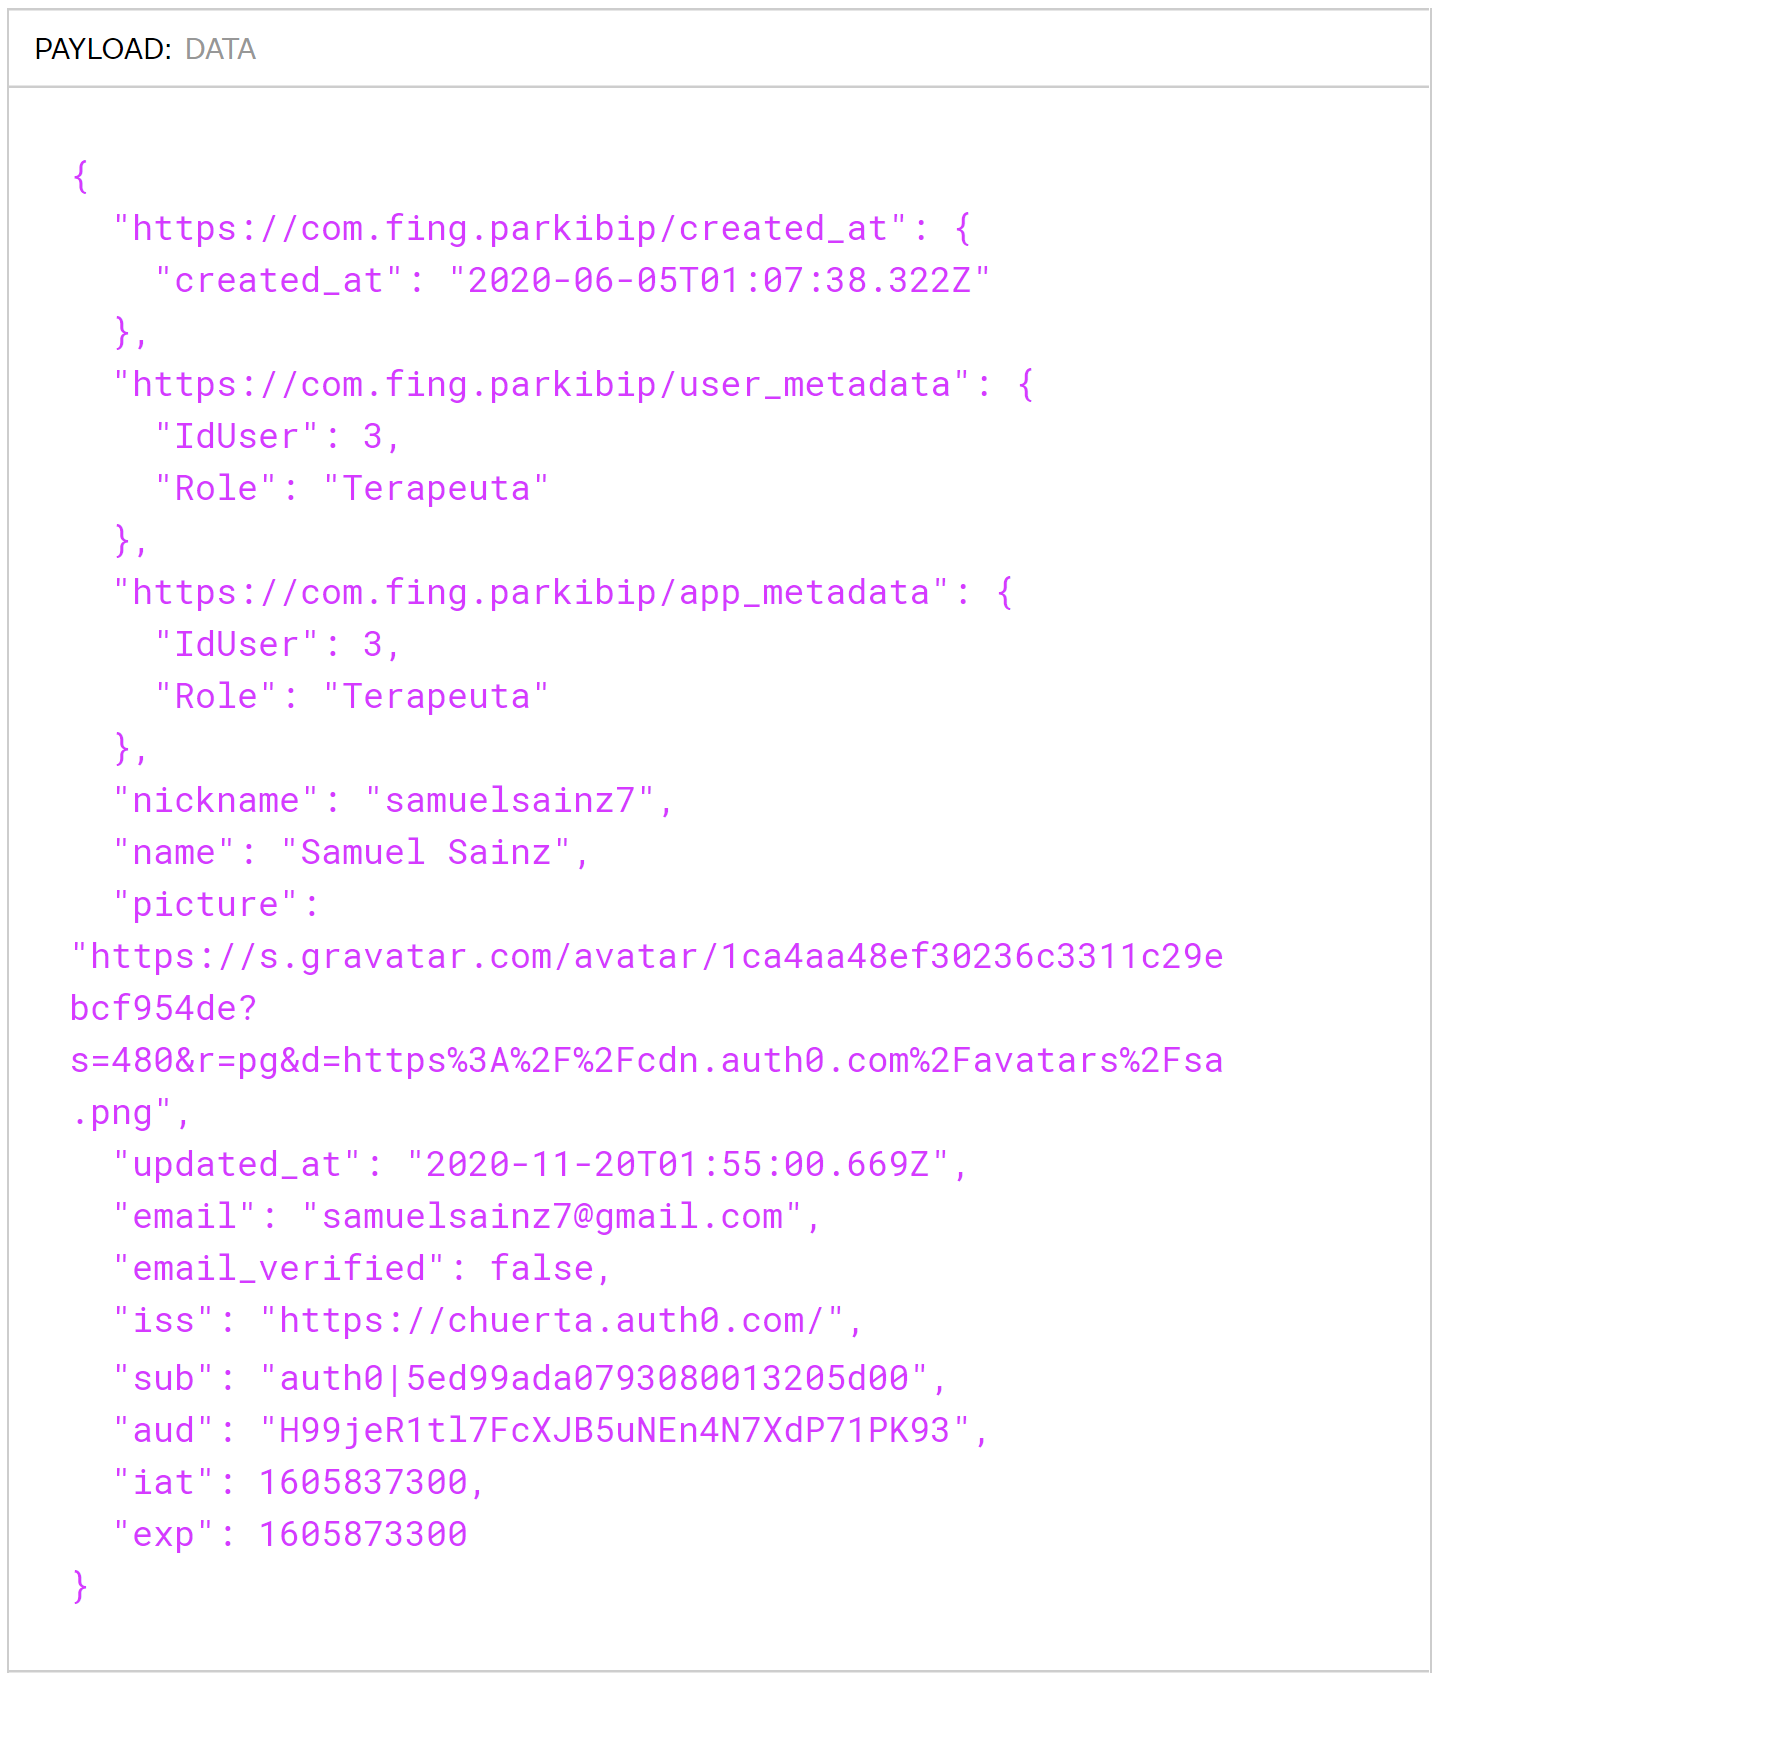
\includegraphics[width=\textwidth]{TESIS/imagenes/chap05/payload-token.PNG}
\caption{Ejemplo de carga útil (del inglés Payload) durante el intercambio de información embebida en el token de identificación. Se aprecian metadatos del usuario, información descriptiva y transaccional (e.g. nombre, email, rol o tipo de usuario en el sistema, etc.)}
\label{FIG:payload-token}
\end{figure}

Asimismo, mediante el decodificador, se puede apreciar el algoritmo criptográfico empleado y el tipo de token generado. Véase la figura Fig. \ref{FIG:header-token}.

\begin{figure}[H]
\centering
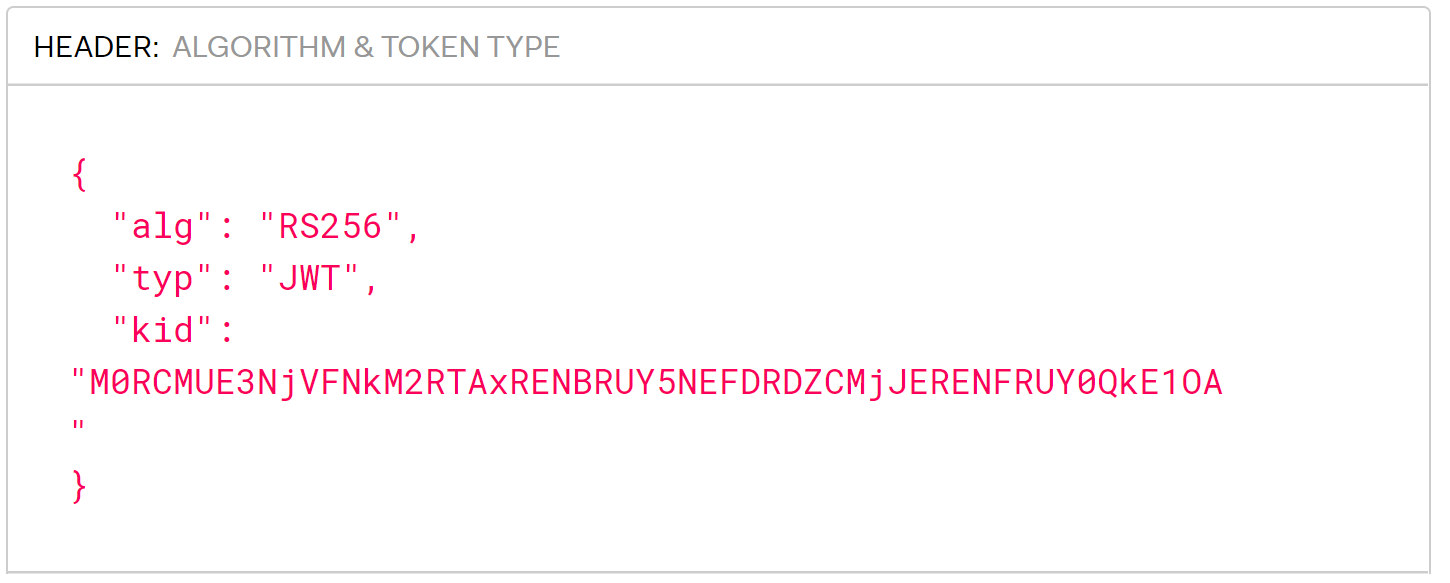
\includegraphics[width=\textwidth]{TESIS/imagenes/chap05/header-token.PNG}
\caption{Ejemplo de encabezado de un token JWT. Especifica el algoritmo de cifrado y el tipo de token generado.}
\label{FIG:header-token}
\end{figure}

A continuación, se mencionan otras tareas de desarrollo relativas al módulo de identidad:
\begin{itemize}
    \item Inclusión de la SDK de Auth0 mediante la dependencia \textit{'com.auth0.android:auth0:1.+'}. La librería encapsula la comunicación con las API de autenticación y administración de Auth0.
    \item Administración de propiedades de acceso: \textit{com\_auth0\_domain}, \textit{com\_auth0\_client\_id}.
    \item \textit{Callback}: Un \textit{callback}, es una URL en la aplicación en donde Auth0 redirige al usuario después de que el mismo se ha autenticado.
    \item \textit{Logout URL}: Una URL de cierre de sesión, es una URL en la aplicación a la que Auth0 puede retornar luego de que el usuario haya cerrado la sesión del servidor de autorización. En PARKIBIP se definió: \textit{fing://parkibip.auth0.com/android/parkibipapp/callback}.
    \item Función Login: Método responsable de realizar el flujo de autenticación y distinción por niveles de usuario (Terapeuta, Paciente).
    \item Función Logout: Método encargado de administrar el cierre de la sesión activa en la aplicación.
    \item Administración de credenciales: Componente responsable de administrar los tipos de tokens de Auth0, por ejemplo, token para actualización -\textit{refresh\_token}-, token de identidad -\textit{id\_token}-, token de acceso -\textit{access\_token}-.
\end{itemize}

El flujo de autenticación empleado a través de Auth0, se basa en \textit{OAuth 2.0}, utilizando una clave de prueba para intercambio de código (del inglés, Proof Key for Code Exchange, conocido por PKCE) La ilustración Fig. \ref{FIG:flow-PKCE}, tomada de \cite{Auth0:PKCE} y adaptada al proyecto, refleja el flujo de intercambios de mensajes durante el proceso de autenticación que efectúa PARKIBIP. 

\begin{figure}[!h]
\resizebox{\textwidth}{!}{
\centering
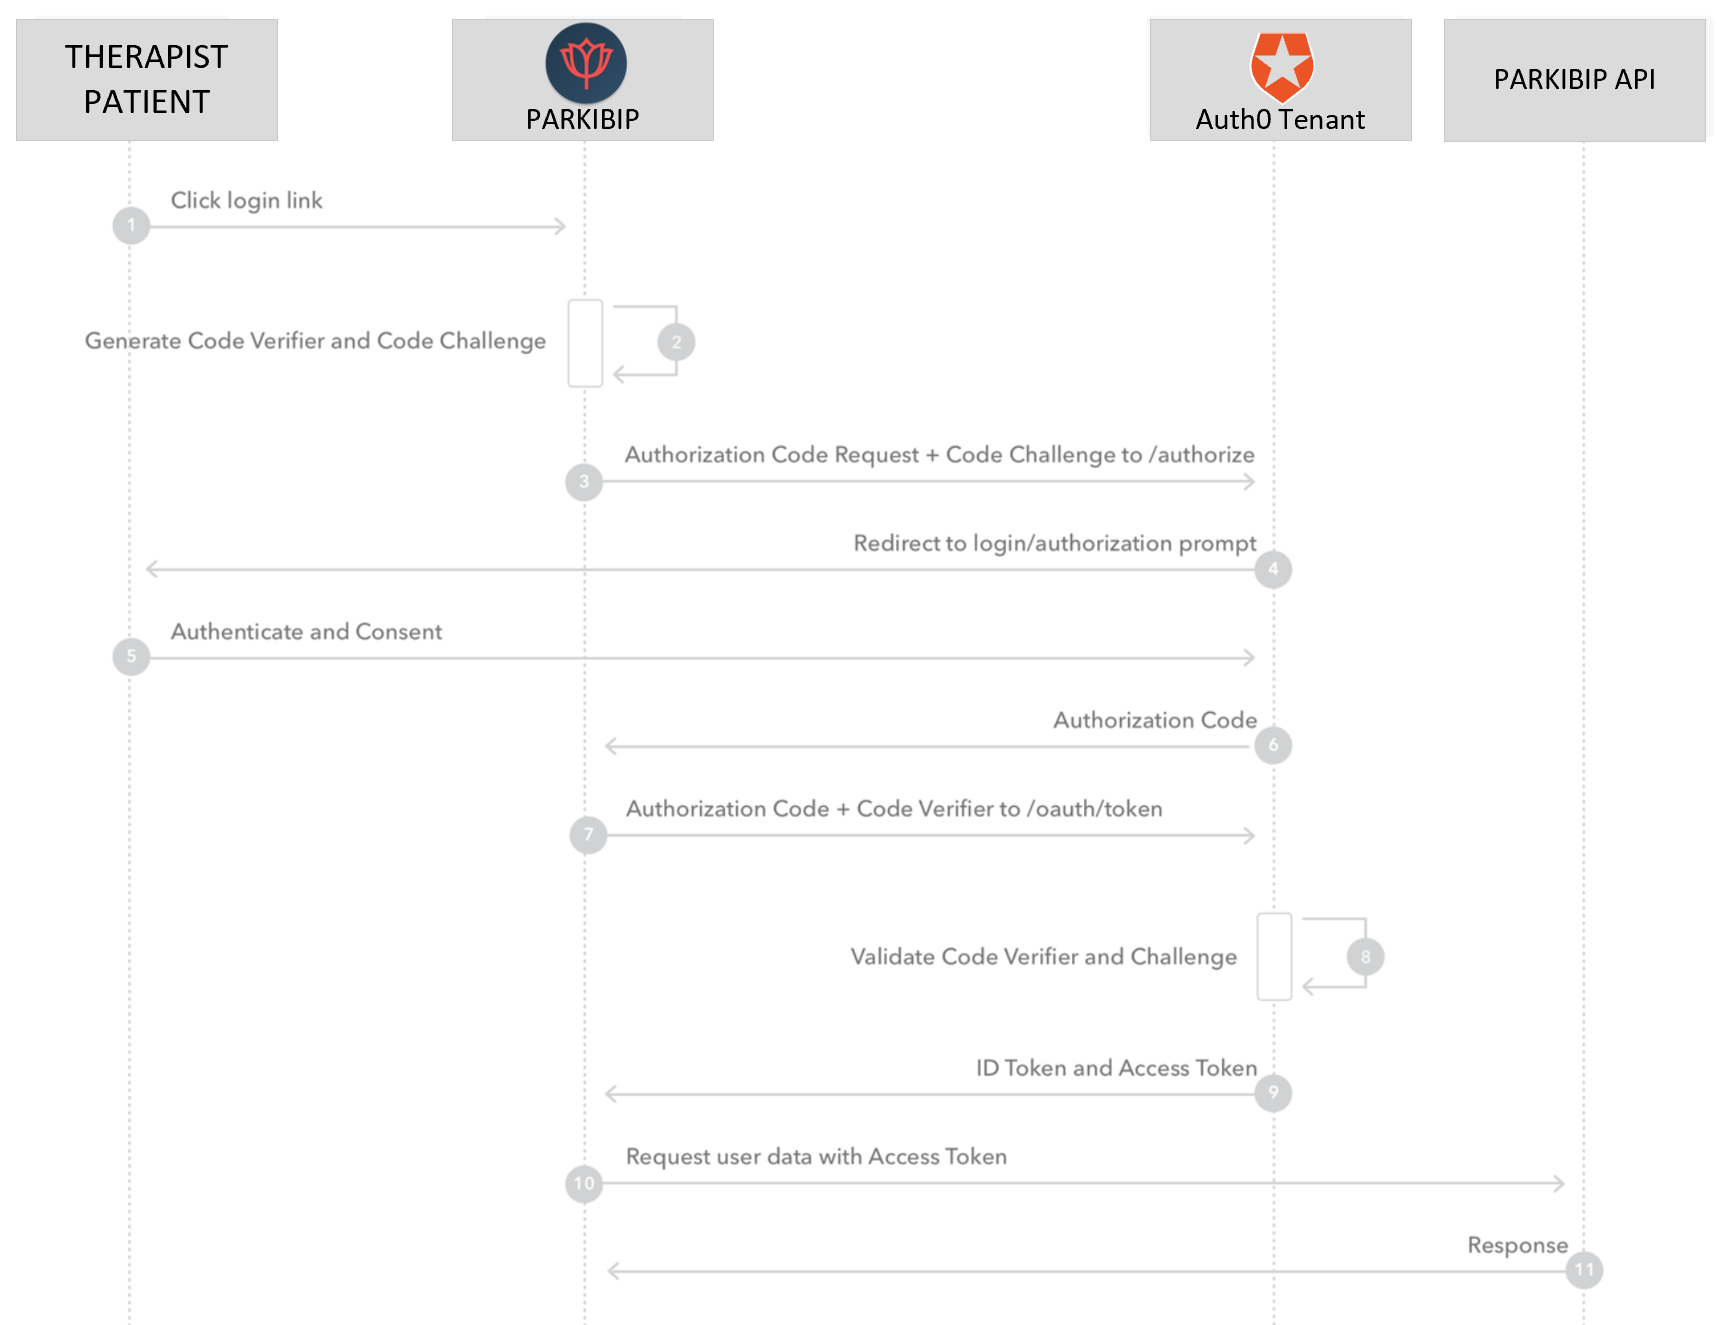
\includegraphics{TESIS/imagenes/chap05/parkibip-auth0-flow.PNG}}
\caption{Flujo de autenticación y autorización entre PARKIBIP y Auth0 Tenant, a través del protocolo clave de prueba para intercambio de código (PKCE). Cita a \cite{Auth0:PKCE} y adaptación a PARKIBIP}
\label{FIG:flow-PKCE}
\end{figure}

En resumen, el procedimiento de autenticación e implícito al usuario sigue el proceso:
\begin{enumerate}
    \item El Paciente o Terapeuta intenta ingresar al sistema, para ello, hace click en Iniciar Sesión dentro de la aplicación.
    \item Mediante la invocación a la función LogIn de el SDK de Auth0, se crea un verificador de código -\textit{code\_verifier}- con cifrado aleatorio y a partir de ésto se genera un desafío de código -\textit{code\_challenge}-.
    \item El SDK en Android redirige al usuario al Servidor de autorización de Auth0 invocando el endpoint \textit{/authorize} de su API, adjuntando el \textit{code\_challenge}.
    \item El servidor de Auth0 redirige al usuario a la solicitud de inicio de sesión y autorización.
    \item Luego, el usuario se autentica utilizando una de las opciones de inicio de sesión pre-establecidas -usuario y contraseña-. En caso de ser el primer inicio de sesión, se despliega una página de consentimiento con los permisos que la aplicación le otorgará a Auth0.
    \item El servidor de autorización, almacena el \textit{code\_challenge}, luego, redirige al usuario a la aplicación con un código.
    \item El SDK envía el código recibido junto a el \textit{code\_verifier} -creado en el paso 2- al servidor de autorización de Auth0, endpoint \textit{/oauth/token}.
    \item El servidor de  autorización de Auth0 verifica los datos  \textit{code\_challenge} y \textit{code\_verifier} enviados.
    \item Finalmente, Auth0 responde con los tres tokens necesarios: \textit{id\_token}, \textit{access\_token}, \textit{refresh\_token}.
\end{enumerate}

Así, cada vez que un usuario intenta autenticarse, Auth0 verifica la identidad y envía la información requerida a PARKIBIP. Para concluir, la imagen Fig. \ref{FIG:idtoken}, brinda un ejemplo de token de identificación -\textit{id\_token}-, resultado de ejecuta el flujo de proceso autenticación y autorización.

\begin{figure}[!h]
\resizebox{\textwidth}{!}{
\centering
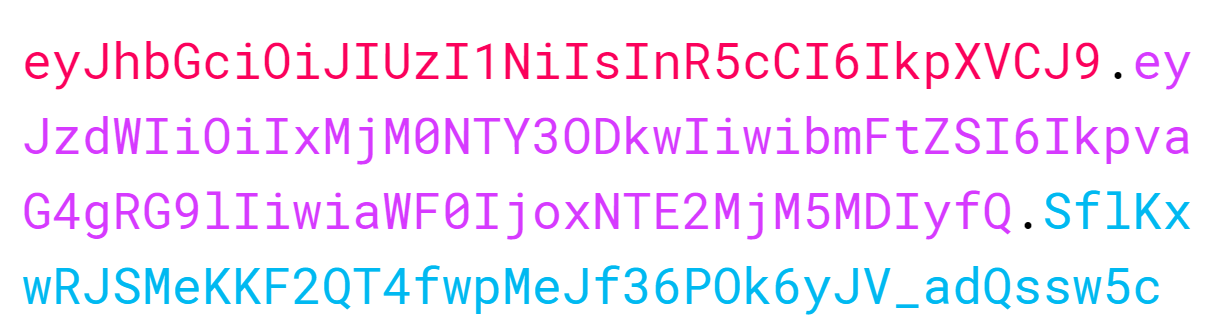
\includegraphics{TESIS/imagenes/chap05/token.PNG}}
\caption{Ejemplo de token de identidad --\textit{id\_token}-- con formato JWT, obtenido como resultado del flujo \ref{FIG:flow-PKCE} }
\label{FIG:idtoken}
\end{figure}

\section{Administración de Terapeutas y Pacientes}

PARKIBIP tiene como propósito la ejecución de sesiones de rehabilitación para un Paciente y coordinadas por un Terapeuta, por consiguiente es imprescindible la administración de Terapeutas y Pacientes. Es necesario llevar el registro de los mismos para asociar las diferentes sesiones de terapia. Mantener los datos de los pacientes, entre otras cosas, permitió el desarrollo de funcionalidades como ser la visualización del listado de los pacientes para un Terapeuta particular, ver sus sesiones, y luego medir el progreso de cada paciente. Dentro de las historias de usuario del sistema, se desea que, tanto los pacientes como los terapeutas, puedan observar la información vinculada a las distintas sesiones, mantener su registro y compararlas para analizar el progreso entre cada sesión. 

La figura Fig. \ref{FIG:users-and-sessions-class-diagram} presenta el diagrama de clases con el diseño de esta sección del sistema. La entidad \textit{User} -Usuario-, representa tanto a los pacientes como a los terapeutas y mantiene la información descriptiva de éstos, como lo es el nombre, el apellido y un identificador único auto-generado en el sistema. Luego, utilizando el concepto de herencia, se extiende la clase \textit{Patient} -Paciente- que además integra datos particulares que se desean conocer para éste nivel de usuario: edad, documento, observaciones relevantes (e.g. ``rigidez en pierna derecha'', ``episodios de FoG'' o cualquier tipo de observación sobre el paciente que sea relevante). Similar, se tiene una entidad \textit{Therapist} -Terapeuta- que hereda de \textit{User}, y además adjunta la información específica de un terapeuta, por ejemplo el centro médico en el cual trabaja. A su vez, \textit{UsersManager} es una componente que tiene el conocimiento para administrar los niveles de usuarios e identificar cuál es el paciente activo para las futuras sesiones. A través de \textit{UsersManager} se pueden obtener los distintos usuarios, agregar un nuevo paciente, recuperar un paciente particular a través de su identificador, etc. 

\begin{figure}[H]
    \hspace*{-2.0cm}%
    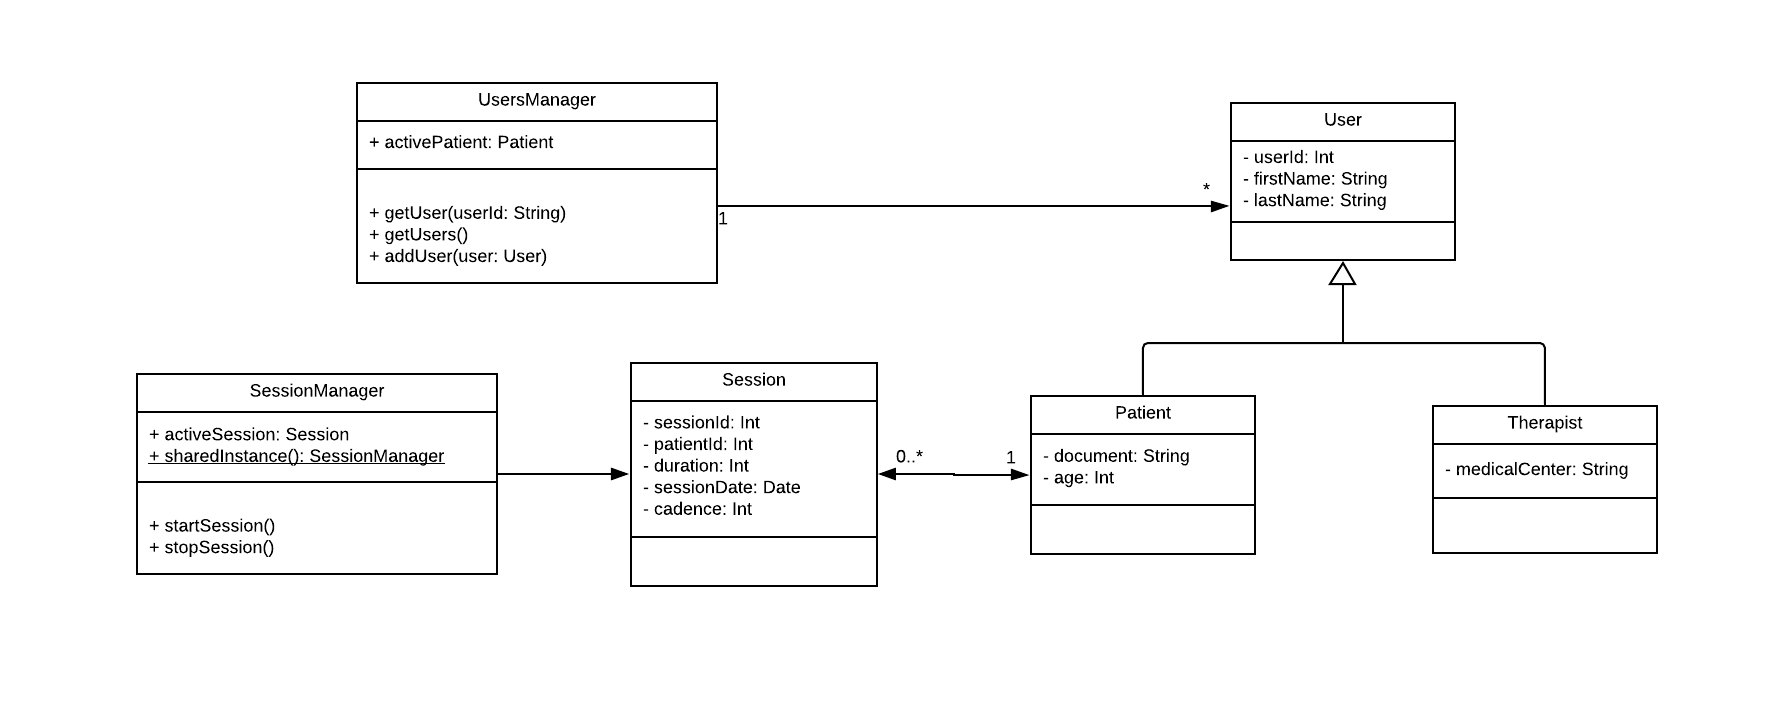
\includegraphics[clip,width=1.25 \columnwidth]{TESIS/imagenes/chap05/users-and-sessions-class-diagram.png}
    \caption{Diagrama de clases del módulo de la aplicación Android donde se representan los terapeutas, pacientes y las sesiones realizadas.}
    \label{FIG:users-and-sessions-class-diagram}
\end{figure} 

Dentro del menú de navegación de la aplicación, para visualizar el listado de pacientes almacenados, se puede consultar el acceso directo ``Perfiles''. La figura Fig. \ref{fig:activity-users}  muestra dicha pantalla. Con el fin de trabajar la amigabilidad del sistema, se le proporciona al usuario la capacidad de filtrar los pacientes utilizando la funcionalidad de búsqueda, accesible a través del icono de búsqueda en la barra superior de navegación de la pantalla. 

\newpage

\begin{figure}[H]
 \centering
 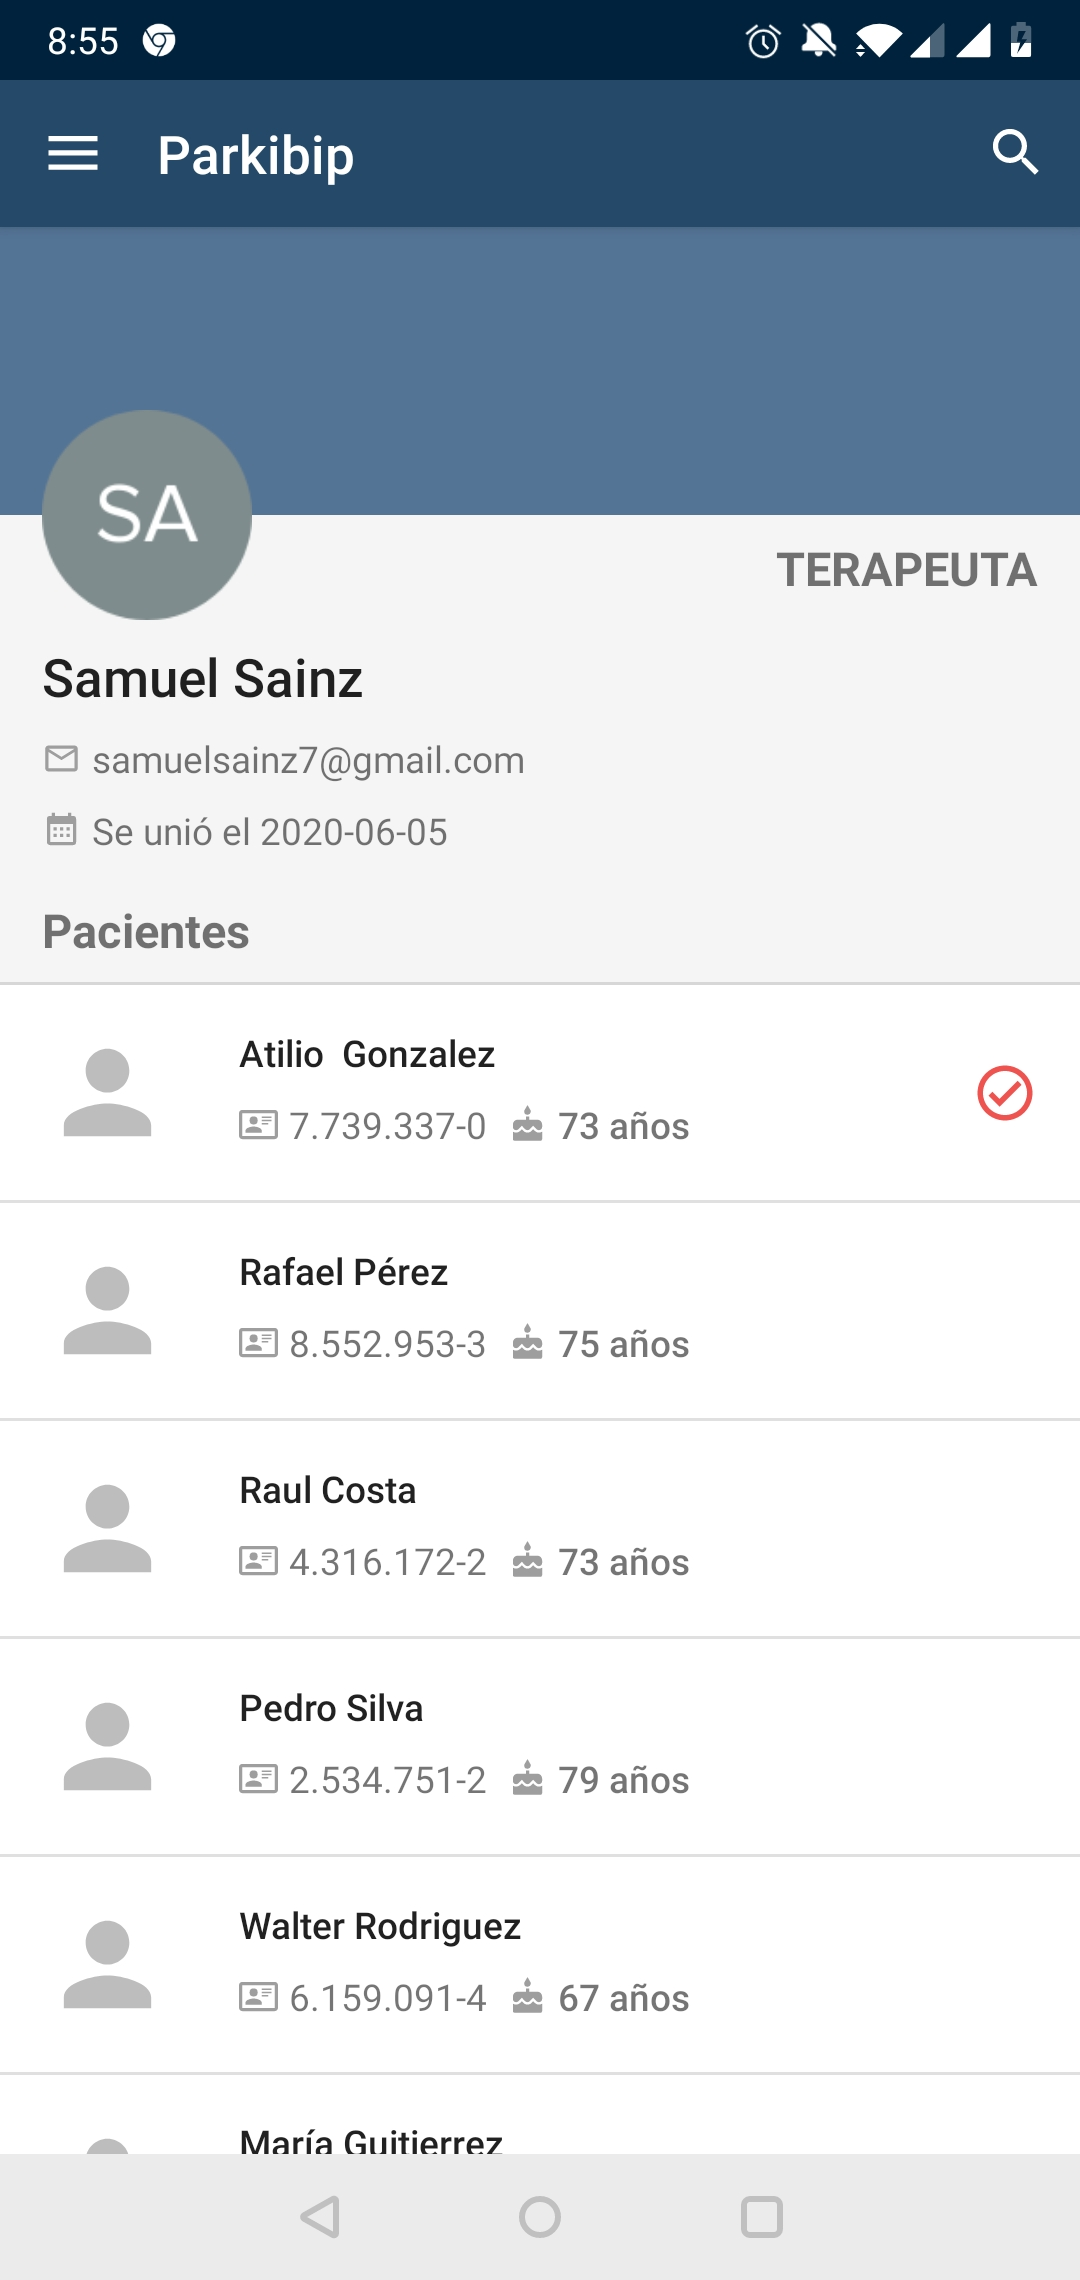
\includegraphics[height=8cm]{TESIS/imagenes/chap05/activity-users.JPG}
 \caption{Visualización de perfiles de usuarios. Funcionalidades: (i) Ver información descriptiva del usuario logueado, (ii) Ver el listado de pacientes -en caso de ser un terapeuta-, (iii) Seleccionar el paciente activo para futuras sesiones de rehabilitación.}
 \label{fig:activity-users}
\end{figure}

\section{Administración de Sesiones de rehabilitación}

PARKIBIP es un sistema rehabilitador en base a sesiones clínicas, por lo tanto, cada paciente tendrá tantas sesiones PARKIBIP -representadas con la clase \textit{Session}- como sesiones de rehabilitación. Para cada una de estas sesiones, se conoce el identificador del paciente que realizó la sesión, la fecha de realización, la duración, así como los parámetros espacio-temporales resultantes de su procesamiento: cadencia, cantidad de pasos, velocidad promedio, duración -ver figura Fig. \ref{fig:activity-summary}-.

\newpage

\begin{figure}[H]
 \centering
 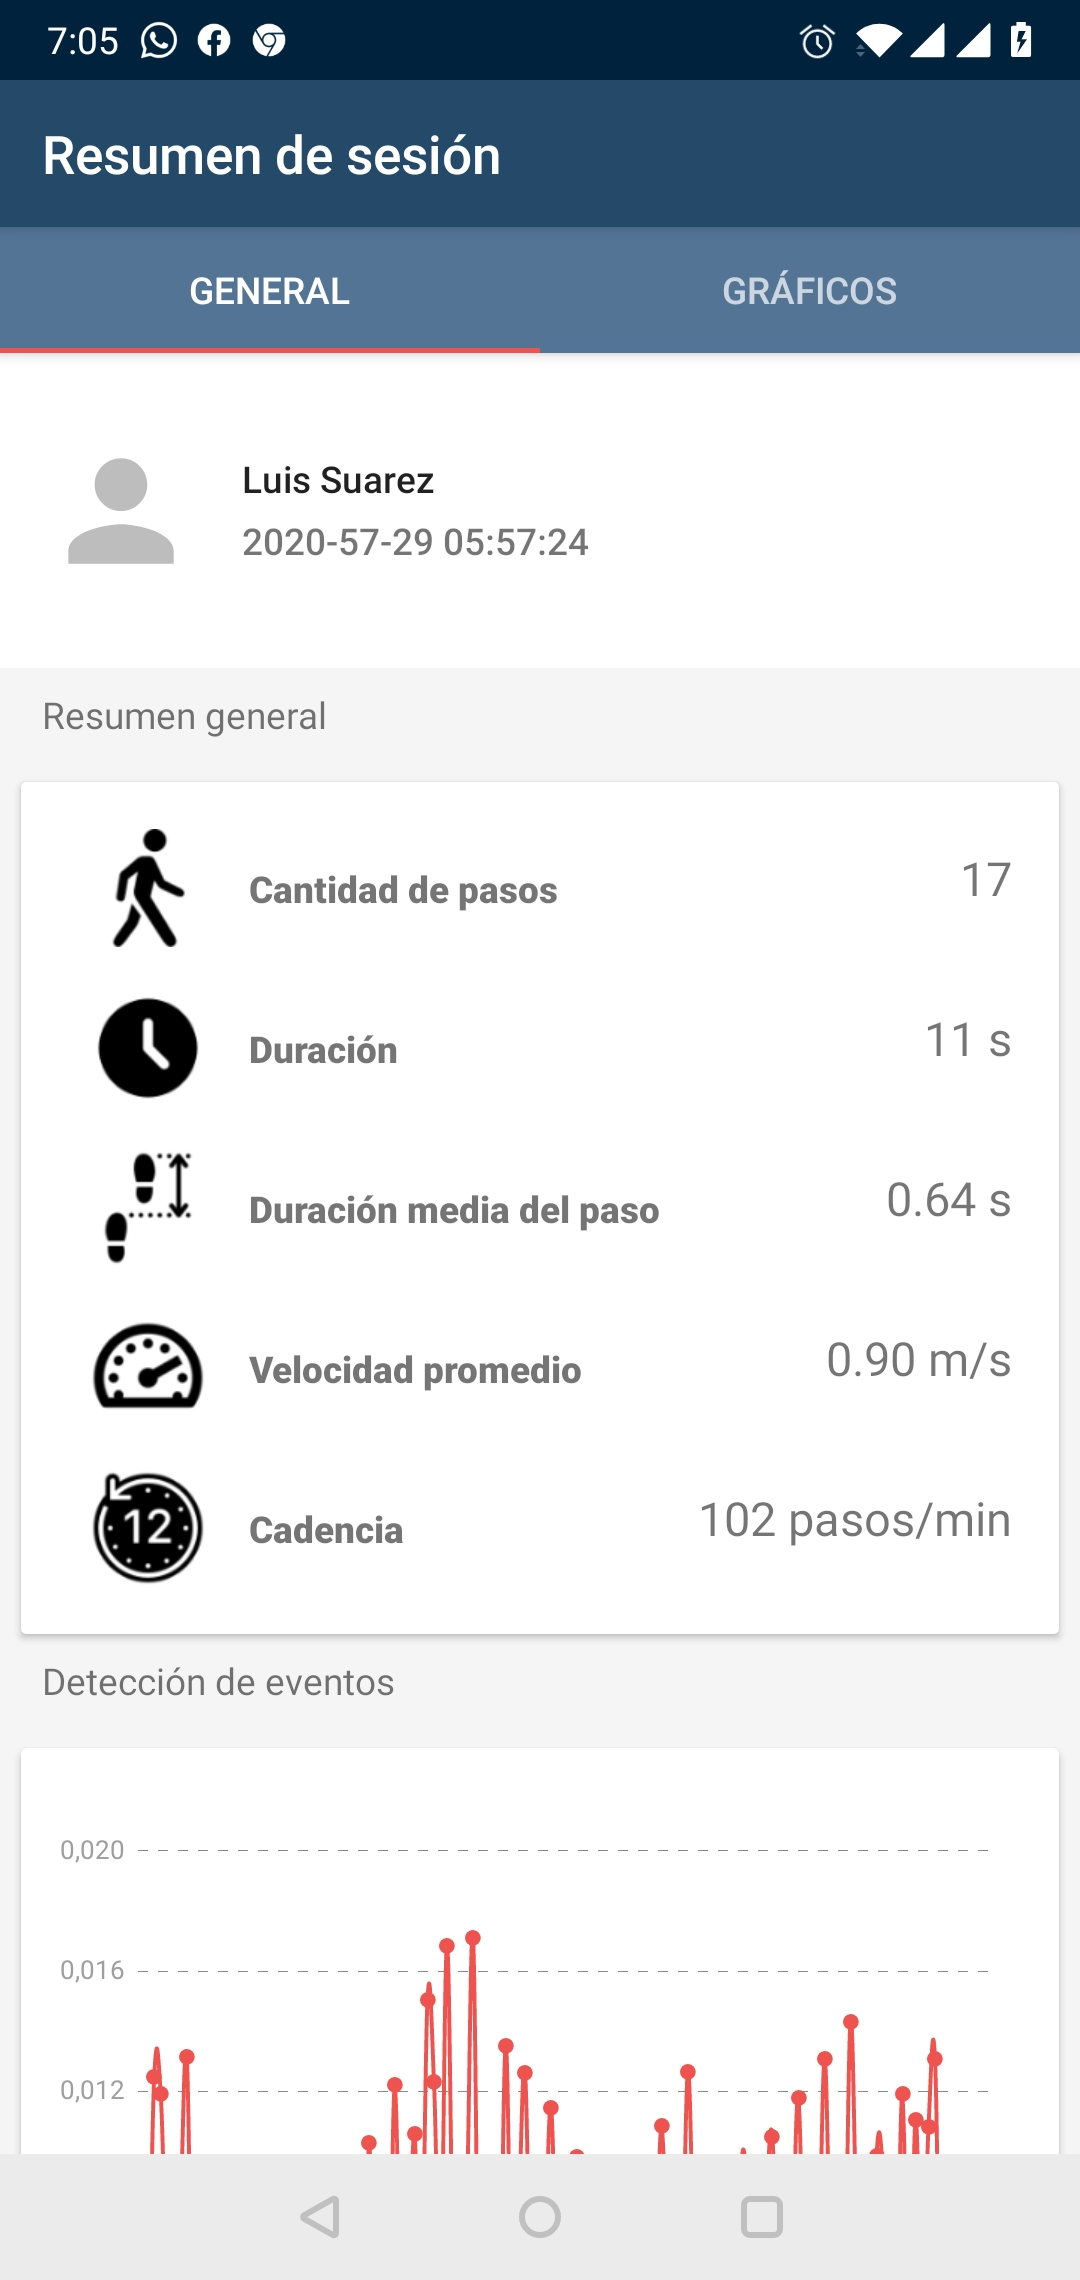
\includegraphics[height=8cm]{TESIS/imagenes/chap05/activity-session-summary.JPG}
 \caption{Resumen general y detallado de una sesión. Se presenta el comportamiento de la marcha en términos de valores de parámetros espacio-temporales y de forma gráfica.}
 \label{fig:activity-summary}
\end{figure}

Por su parte, el componente \textit{SessionsManager} es la clase encargada de administrar las sesiones realizadas, tiene la responsabilidad de crear, listar, remover sesiones, y sobretodo identificar una sesión viva. Durante una sesión PARKIBIP, es el \textit{SessionsManager} quien mantiene la instancia de sesión activa, útil para guardar en la sesión en la base de datos finalizada la sesión, combinarla con las mediciones y con los resultados del post-procesamiento. 

Una vez que la sesión es completada, se almacena en la base de datos el resumen genérico y detallado de la misma, generando una pantalla específica en la aplicación conforme a medir los resultados logrados. Además, dicha sesión se puede encontrar en el historial de sesiones de la aplicación, a través del menú de navegación de la aplicación, acceso ``Historial de sesiones''. La figura Fig. \ref{fig:activity-history-session} visualiza dicha pantalla. 

\newpage

\begin{figure}[H]
 \centering
 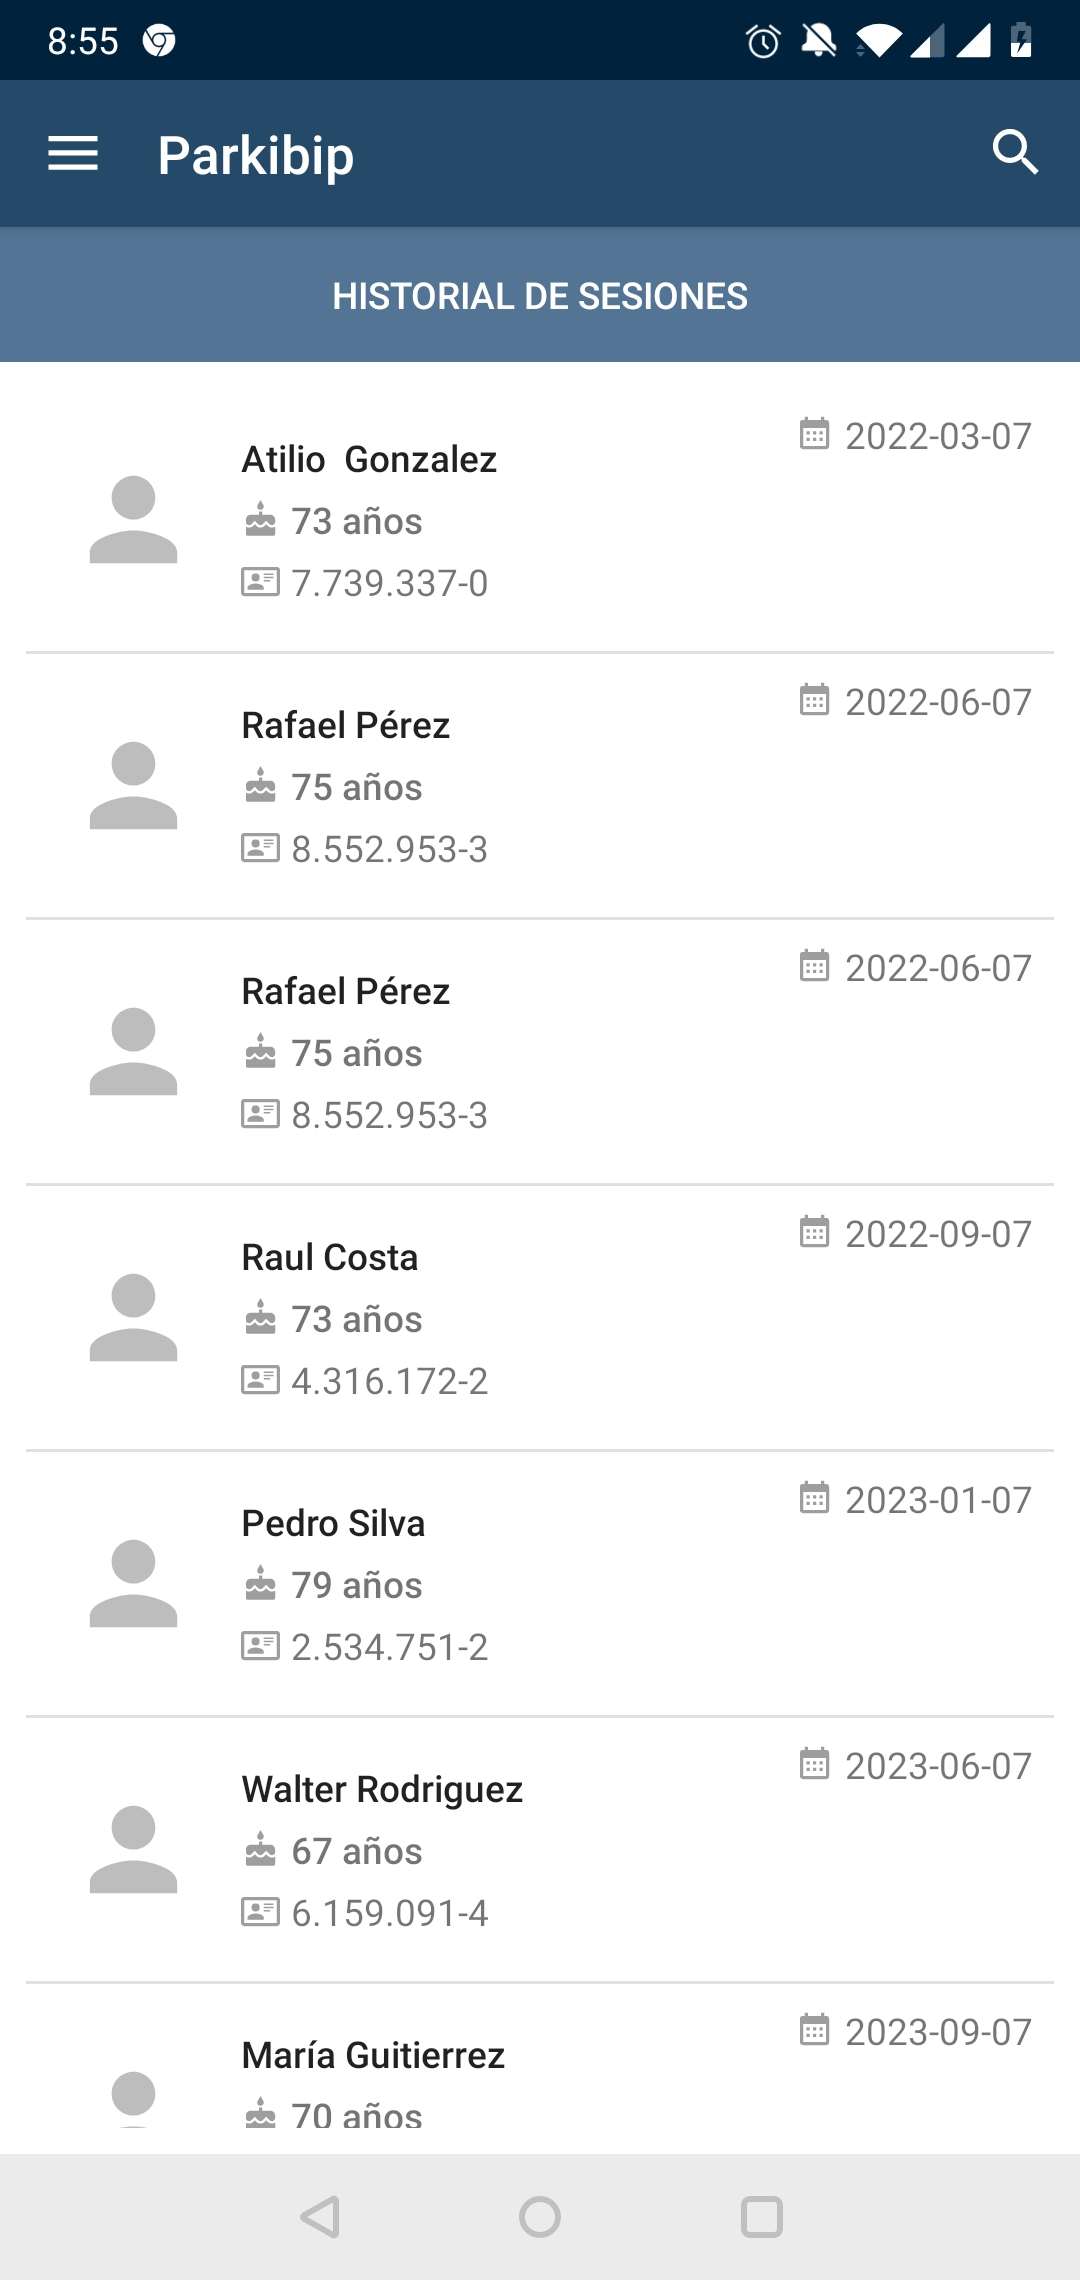
\includegraphics[height=8cm]{TESIS/imagenes/chap05/session-list.jpg}
 \caption{Historial de sesiones. Ordenadas cronológicamente con su correspondiente fecha de realización y paciente evaluado. Permite acceder a su resumen mediante su selección.}
 \label{fig:activity-history-session}
\end{figure}

Cada una de las sesiones listadas, presenta la información del paciente que realizó la sesión. Adicionalmente, el usuario puede filtrar las sesiones digitando el nombre del paciente en la barra de búsqueda situada en la parte superior de la pantalla. Respecto a las sesiones, también se conocen las mediciones y los resultados de los procesamientos realizados en el transcurso de toda la sesión. En la pantalla donde se resume la sesión, se pueden ver las gráficas detalladas en función del tiempo: velocidad, trayectoria y aceleración.


\section{Diagrama de clases}

El objetivo de esta sección es, presentar el diseño de la aplicación Android mediante un diagrama de clases simplificado, ilustrado en la figura Fig. \ref{FIG:class-diagram-design}. Si bien, por simplicidad, se omiten algunas entidades del sistema, en el siguiente diagrama se pueden ver los elementos fundamentales de la aplicación móvil. El diagrama brinda una visión general de cómo está diseñado el sistema, así como sus responsabilidades y la interacción entre ellos.

\newpage

\begin{figure}[H]
    \hspace*{-2.0cm}%
    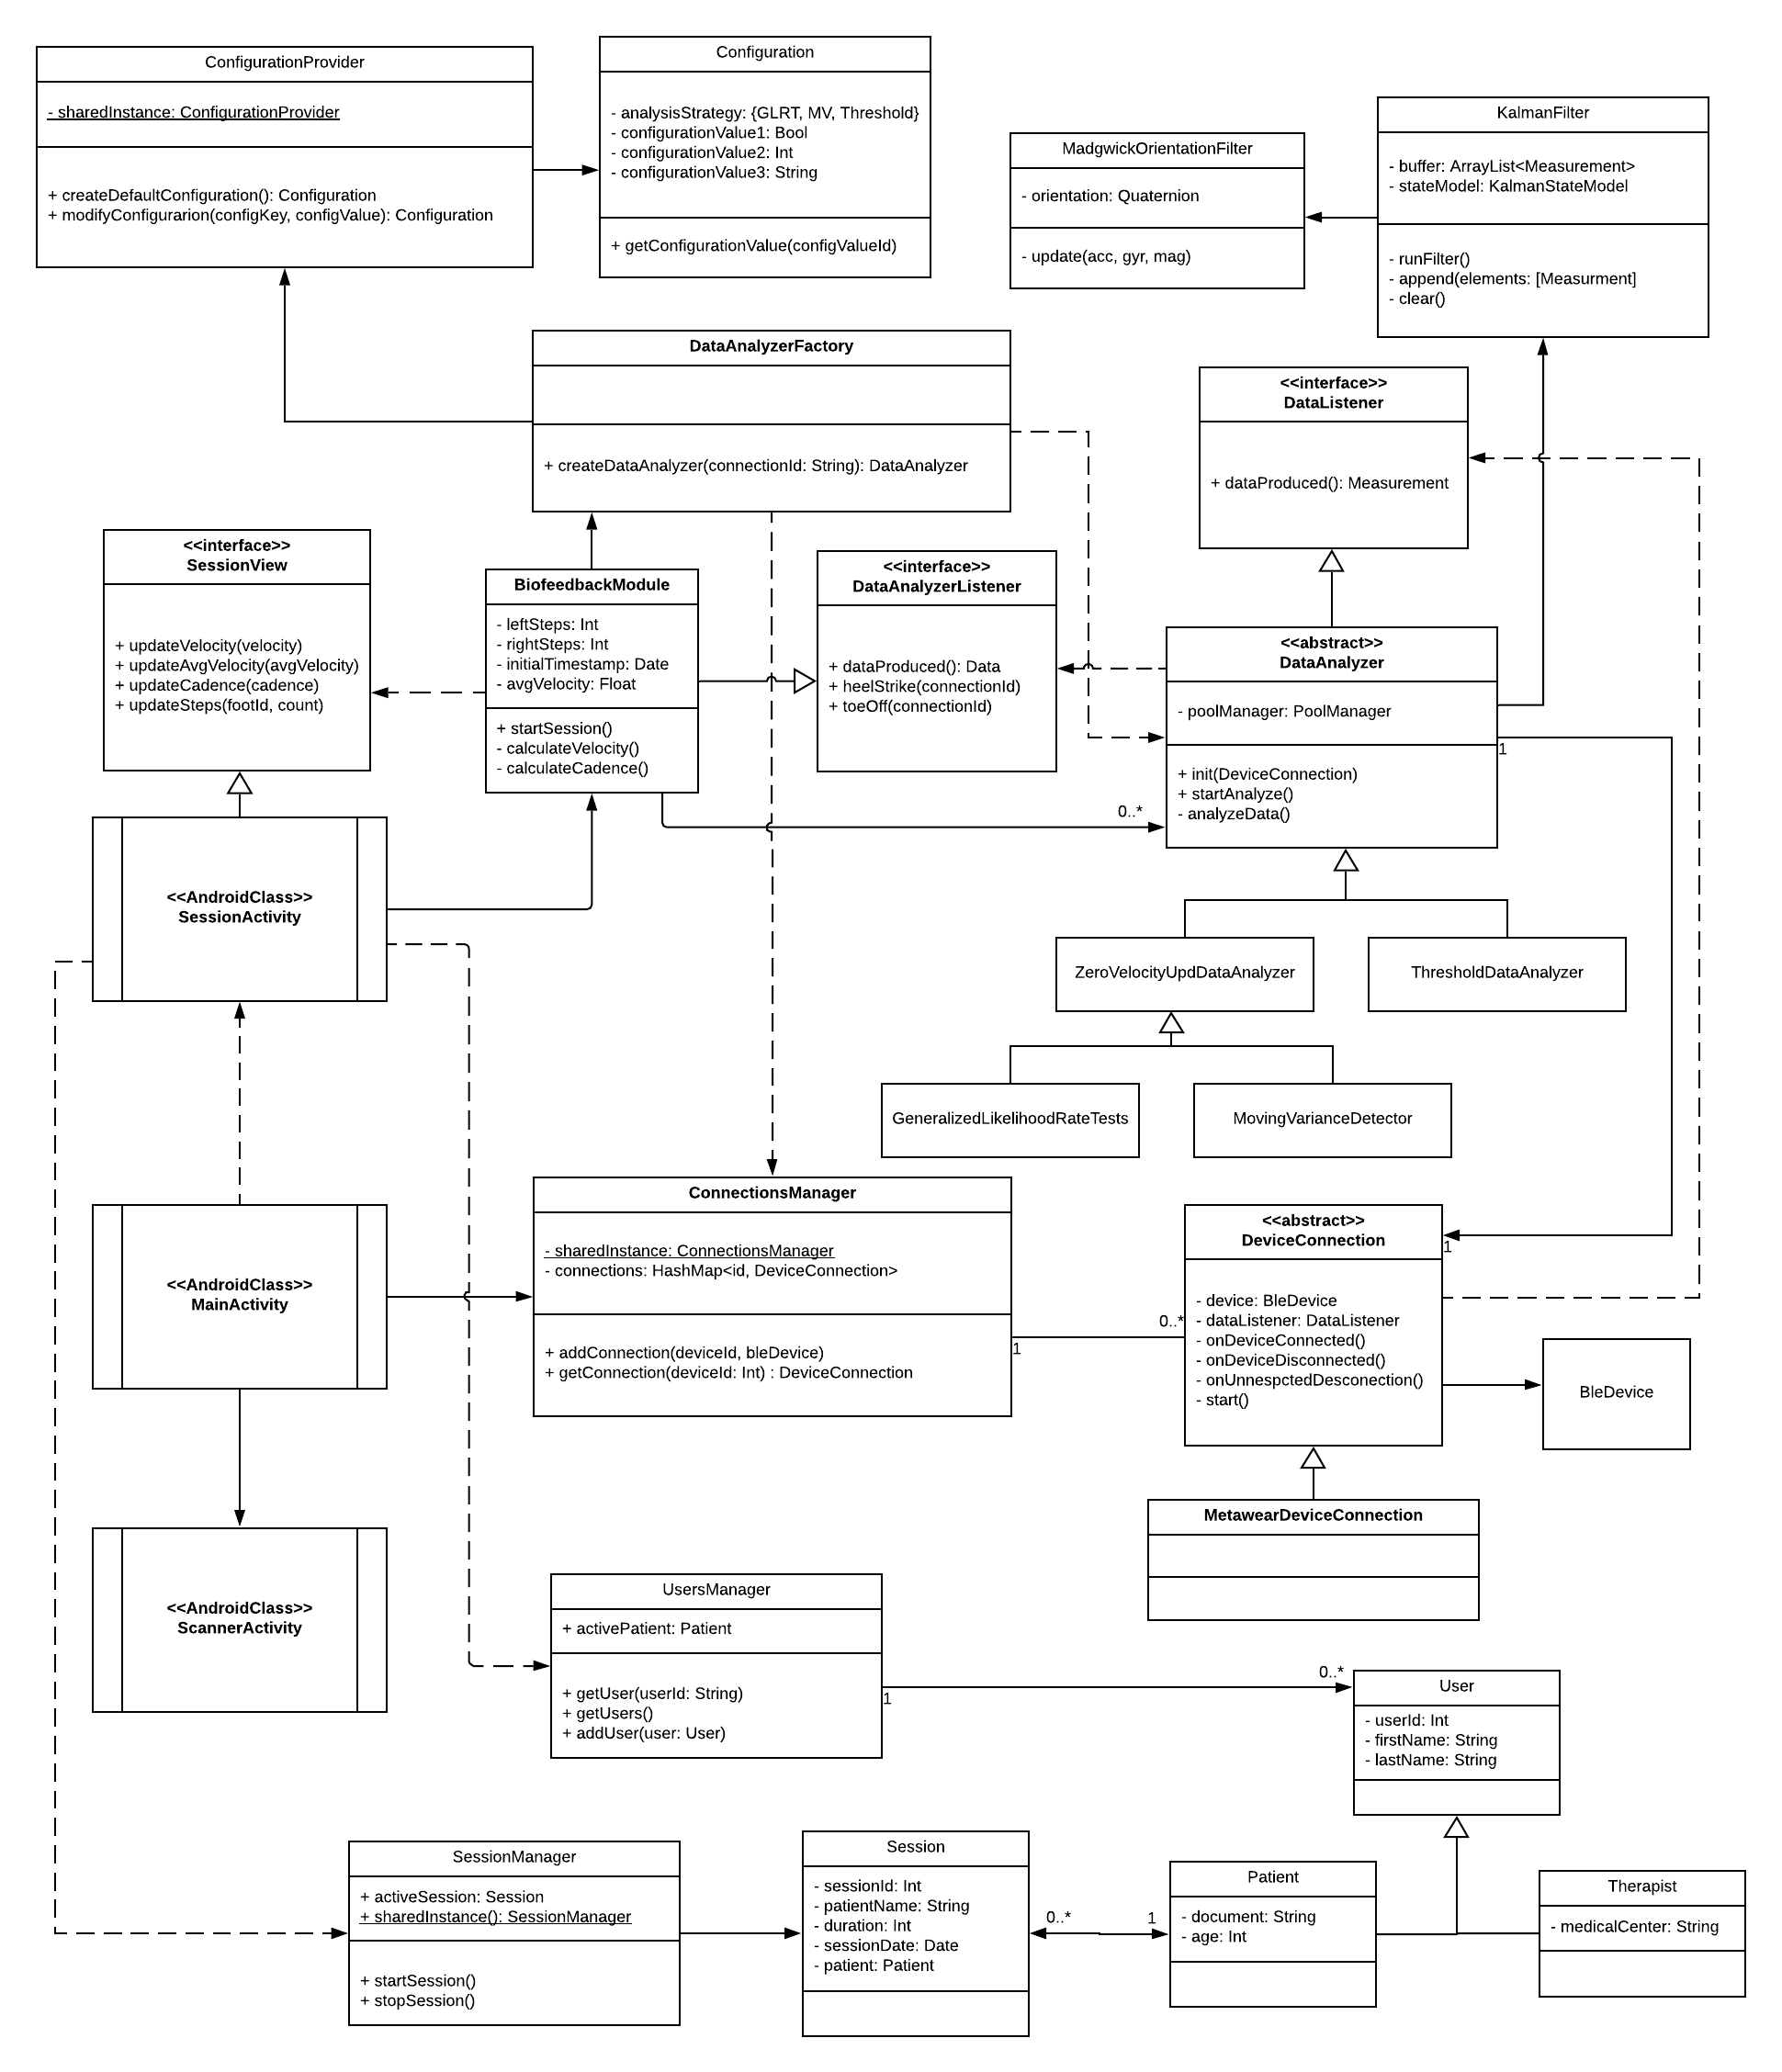
\includegraphics[clip,width=1.25 \columnwidth]{TESIS/imagenes/chap05/Parkibip-Design.png}
    \caption{Diagrama de clases de la aplicación Android PARKIBIP. Se muestran en este diagrama los componentes esenciales del sistema y se omiten varios por simplicidad.}
    \label{FIG:class-diagram-design}
\end{figure}

Para diseñar PARKIBIP se tuvieron en cuenta varios principios de diseño que favorecen las cualidades del sistema como mantenibilidad, escalabilidad, calidad, entre otras. Como se puede ver en el diagrama, existe una alta cohesión de los componentes y un bajo acoplamiento entre éstos. Se intentó no repetir código, mantener responsabilidades únicas, abstraer comportamiento mediante interfaces y clases abstractas. En PARKIBIP se tuvieron en cuenta los principios de diseño SOLID. SOLID es un acrónimo que resume los cinco principios de diseño de diagramas de clases\cite{Chebanyuk2016}:

\begin{itemize}
    \item \textbf{S}ingle Responsibility: Responsabilidad única
    \item \textbf{O}pen-Closed: Abierto-Cerrado
    \item \textbf{L}iskov Substitution: Principio de Sustitución de Liskov
    \item \textbf{I}nterface Segregation: Principio de Segregación de Interfaces
    \item \textbf{D}ependency Inversion: Inversión de la Dependencia 
\end{itemize}

El principio de \textbf{responsabilidad única} es quizás el más simple de identificar observando el diagrama de clases, ya que es fácil notar que cada clase del sistema tiene una única función u objetivo. Para mencionar un ejemplo, se puede ver que \textit{ConfigurationProvider} es encargado de proveer las configuraciones, administrarlas, modificarlas, etc; pero la configuración en sí está dada por la clase \textit{Configuration}. \textit{DataAnalyzerFactory} es una clase que consulta a \textit{ConfigurationProvider} por una instncia de \textit{Configuration} para poder crear la instancia de \textit{DataAnalyzer} que corresponda. Como se puede ver, cada uno de los actores tiene una única responsabilidad y ésto está reflejado en \textbf{todas} las clases del sistema. 

Por otro lado, se tuvo en cuenta también el principio \textbf{Open-Closed}, que consiste en lo siguiente: ``Las entidades de software (clases, módulos, funciones, etc.) deben estar abiertas para su extensión, pero cerradas para modificaciones''. Esto se ve reflejado en el diseño de PARKIBIP de forma clara en la implementación de las conexiones para cada dispositivo, donde se define el comportamiento en la clase \textit{DeviceConnection} y se extiende el mismo para el dispositivo \textit{MetaMotionR} en la clase \textit{MetaWearDeviceConnection}. Esto permite que el sistema sea fácilmente escalable o extensible a otros proveedores de hardware, que sea mantenible y que además se pueda reutilizar código. También se aplicó este principio en la implementación de los algoritmos de análisis de los datos para detección de eventos, en la definición de usuarios, entre otros. 

El principio de sustitución de Liskov complementa el principio de Open-Closed, y lo vemos aplicado en PARKIBIP en los mismos elementos que éste. El principio define que los objetos de una superclase serán reemplazables por objetos de sus subclases sin interrumpir la aplicación. Eso requiere que los objetos de sus subclases se comporten de la misma manera que los objetos de su superclase. 

El principio de \textbf{segregación de interfaces} dice que ``No se debe obligar a los clientes a depender de interfaces que no utilicen''. En PARKIBIP esto se cumplió complementando el principio de responsabilidad única, ya que se declararon las interfaces encapsulando una única funcionalidad por lo que ningún componente implementa una interfaz con funcionalidades que no utiliza. 

\textbf{Dependency Inversion} refiere a lo que se conoce como inyección de dependencias. Es decir, si cierta clase depende de otro componente, esta dependencia debe ser inyectada en su constructor. Esto permite que las clases sean más testeables a la hora de realizar tests unitarios, donde es necesario aislar su funcionalidad para no depender de otros componentes. La inyección de dependencia nos permite este aislamiento, ya que para los tests unitarios podemos construir nuestra clase inyectando dependencias simuladas. Esto lo utilizamos repetidamente en PARKIBIP inyectando el Contexto de la aplicación Android. Context es una interfaz con información global sobre el entorno de la aplicación. Esta es una clase abstracta cuya implementación es proporcionada por el sistema Android. Permite el acceso a clases y recursos específicos de la aplicación, así como llamadas ascendentes para operaciones a nivel de la aplicación, como actividades de lanzamiento, transmisión y recepción de Intents, etc. \cite{AndroidContext}.

\section{SQLite: Almacenamiento de datos}

Con el fin de gestionar el principal volumen de información, resultante de las sucesivas mediciones de datos obtenidos por los diversos sensores, se optó por implementar una base de datos que actúe local al dispositivo móvil. Almacenar los datos maestros (e.g. algoritmos de detección, parámetros, configuraciones y meta-data), como también los transaccionales (e.g. mediciones, estados de Kalman Filter o actualizaciones de Zero Velocity) en una base de datos es ideal en PARKIBIP para lograr:

\begin{itemize}
    \item Estructurar la información.
    \item Facilitar el procesamiento de la información.
    \item Aumentar o nivelar el rendimiento del sistema -computo sincrónico y asincrónico-, en particular dispositivos con baja capacidad de computo.
    \item Accesibilidad a datos repetitivos.
    \item Centralizar e integrar los datos provenientes de múltiples fuentes -dispositivos IMU y sensores inerciales-.
    \item Gestionar un elevado volumen de datos -en memoria seria inviable-. Por ejemplo, frecuencias altas desde 600 Hz.
\end{itemize}

Se desarrolló una base de datos en el lenguaje estándar SQL, en Android denominado SQLite. Este motor de base de datos liviano de SQL, fue diseñado específicamente para mejorar el rendimiento de sistemas con poca capacidad de procesamiento y almacenamiento. Las APIs requeridas para utilizar una base de datos en Android están disponibles en el paquete \textit{android.database.sqlite}. 

Uno de los principios fundamentales de las bases de datos SQL es la especificación, mediante el modelado de un esquema entidad-relación: una declaración formal de la manera en la que la base de datos está organizada. El diagrama Fig. \ref{FIG: database-mer}, permite visualizar las principales entidades conceptuales y sus relaciones, que luego brindan soporte al sistema PARKIBIP. 

\newpage

\begin{figure}[H]
    \centering
    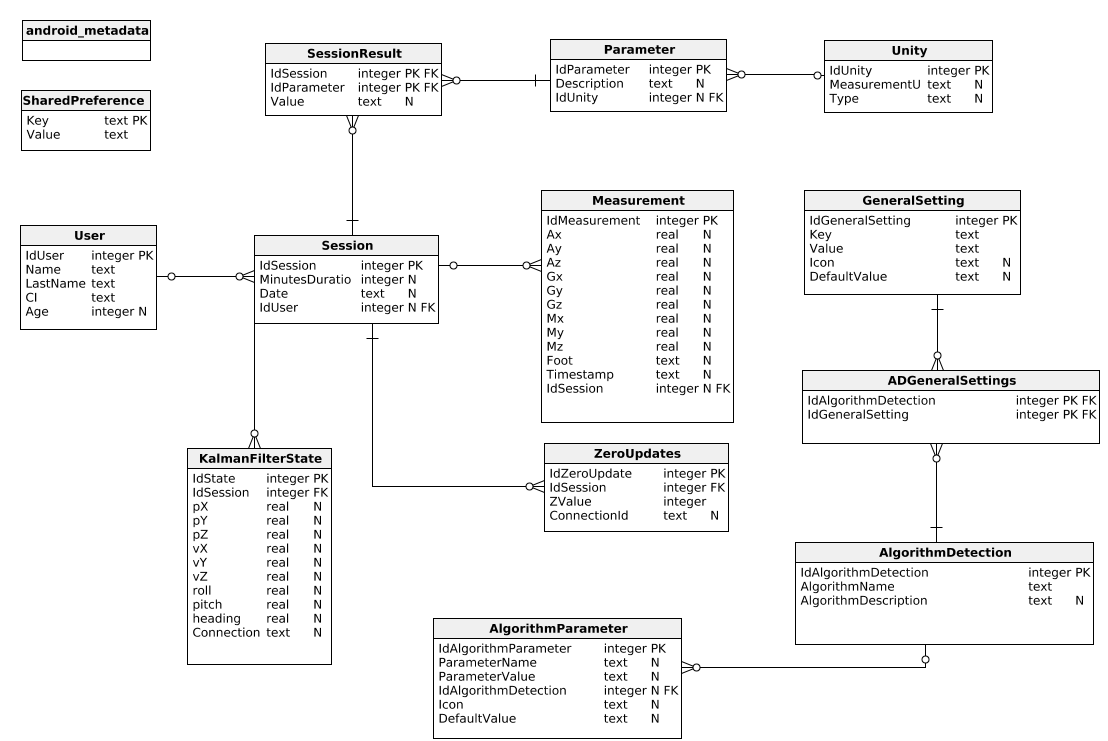
\includegraphics[clip,width=1.1 \columnwidth]{TESIS/imagenes/chap05/database-mer.png}
    \caption{Modelo conceptual entidad-relación de PARKIBIP en Android.}
    \label{FIG: database-mer}
\end{figure}

Así, en el lenguaje Java de Android, resulta útil crear una clase complementaria, denominada clase de contratos -\textit{ParkibipContract}-, que indica explícitamente el diseño del esquema de forma sistemática y auto-documentada. Asimismo, facilita y estandariza el acceso a los datos estructurados mediante el flujo de actividades.

Por otro lado, de forma paralela, se empleó el Software ``DB Browser for SQLite'', siendo la herramienta principal para la gestión de bases de datos en el mencionado lenguaje. Durante el desarrollo, fue provechoso conectarse a la instancia para chequear consistencias, manipular los registros, crear tablas y relaciones, generar restricciones entre los datos, entre otras tareas.

En el apéndice \nameref{anexo:db-tables} se presentan las estructuras de las entidades contempladas en el modelo conceptual. 